%&preformat-disser
\RequirePackage[l2tabu,orthodox]{nag} % Раскомментировав, можно в логе получать рекомендации относительно правильного использования пакетов и предупреждения об устаревших и нерекомендуемых пакетах
% Формат А4, 14pt (ГОСТ Р 7.0.11-2011, 5.3.6)
\documentclass[a4paper,14pt,oneside,openany]{memoir}

%%%%%%%%%%%%%%%%%%%%%%%%%%%%%%%%%%%%%%%%%%%%%%%%%%%%%%
%%%% Файл упрощённых настроек шаблона диссертации %%%%
%%%%%%%%%%%%%%%%%%%%%%%%%%%%%%%%%%%%%%%%%%%%%%%%%%%%%%

%%% Инициализирование переменных, не трогать!  %%%
\newcounter{intvl}
\newcounter{otstup}
\newcounter{contnumeq}
\newcounter{contnumfig}
\newcounter{contnumtab}
\newcounter{pgnum}
\newcounter{chapstyle}
\newcounter{headingdelim}
\newcounter{headingalign}
\newcounter{headingsize}
%%%%%%%%%%%%%%%%%%%%%%%%%%%%%%%%%%%%%%%%%%%%%%%%%%%%%%

%%% Область упрощённого управления оформлением %%%

%% Интервал между заголовками и между заголовком и текстом %%
% Заголовки отделяют от текста сверху и снизу
% тремя интервалами (ГОСТ Р 7.0.11-2011, 5.3.5)
\setcounter{intvl}{3}               % Коэффициент кратности к размеру шрифта

%% Отступы у заголовков в тексте %%
\setcounter{otstup}{0}              % 0 --- без отступа; 1 --- абзацный отступ

%% Нумерация формул, таблиц и рисунков %%
% Нумерация формул
\setcounter{contnumeq}{0}   % 0 --- пораздельно (во введении подряд,
                            %       без номера раздела);
                            % 1 --- сквозная нумерация по всей диссертации
% Нумерация рисунков
\setcounter{contnumfig}{0}  % 0 --- пораздельно (во введении подряд,
                            %       без номера раздела);
                            % 1 --- сквозная нумерация по всей диссертации
% Нумерация таблиц
\setcounter{contnumtab}{1}  % 0 --- пораздельно (во введении подряд,
                            %       без номера раздела);
                            % 1 --- сквозная нумерация по всей диссертации

%% Оглавление %%
\setcounter{pgnum}{1}       % 0 --- номера страниц никак не обозначены;
                            % 1 --- Стр. над номерами страниц (дважды
                            %       компилировать после изменения настройки)
\settocdepth{subsection}    % до какого уровня подразделов выносить в оглавление
\setsecnumdepth{subsection} % до какого уровня нумеровать подразделы


%% Текст и форматирование заголовков %%
\setcounter{chapstyle}{1}     % 0 --- разделы только под номером;
                              % 1 --- разделы с названием "Глава" перед номером
\setcounter{headingdelim}{1}  % 0 --- номер отделен пропуском в 1em или \quad;
                              % 1 --- номера разделов и приложений отделены
                              %       точкой с пробелом, подразделы пропуском
                              %       без точки;
                              % 2 --- номера разделов, подразделов и приложений
                              %       отделены точкой с пробелом.

%% Выравнивание заголовков в тексте %%
\setcounter{headingalign}{0}  % 0 --- по центру;
                              % 1 --- по левому краю

%% Размеры заголовков в тексте %%
\setcounter{headingsize}{0}   % 0 --- по ГОСТ, все всегда 14 пт;
                              % 1 --- пропорционально изменяющийся размер
                              %       в зависимости от базового шрифта

%% Подпись таблиц %%

% Смещение строк подписи после первой строки
\newcommand{\tabindent}{0cm}

% Тип форматирования заголовка таблицы:
% plain --- название и текст в одной строке
% split --- название и текст в разных строках
\newcommand{\tabformat}{plain}

%%% Настройки форматирования таблицы `plain`

% Выравнивание по центру подписи, состоящей из одной строки:
% true  --- выравнивать
% false --- не выравнивать
\newcommand{\tabsinglecenter}{false}

% Выравнивание подписи таблиц:
% justified   --- выравнивать как обычный текст («по ширине»)
% centering   --- выравнивать по центру
% centerlast  --- выравнивать по центру только последнюю строку
% centerfirst --- выравнивать по центру только первую строку (не рекомендуется)
% raggedleft  --- выравнивать по правому краю
% raggedright --- выравнивать по левому краю
\newcommand{\tabjust}{justified}

% Разделитель записи «Таблица #» и названия таблицы
\newcommand{\tablabelsep}{~\cyrdash\ }

%%% Настройки форматирования таблицы `split`

% Положение названия таблицы:
% \centering   --- выравнивать по центру
% \raggedleft  --- выравнивать по правому краю
% \raggedright --- выравнивать по левому краю
\newcommand{\splitformatlabel}{\raggedleft}

% Положение текста подписи:
% \centering   --- выравнивать по центру
% \raggedleft  --- выравнивать по правому краю
% \raggedright --- выравнивать по левому краю
\newcommand{\splitformattext}{\raggedright}

%% Подпись рисунков %%
%Разделитель записи «Рисунок #» и названия рисунка
\newcommand{\figlabelsep}{~\cyrdash\ }  % (ГОСТ 2.105, 4.3.1)
                                        % "--- здесь не работает

%%% Цвета гиперссылок %%%
% Latex color definitions: http://latexcolor.com/
\definecolor{linkcolor}{rgb}{0.9,0,0}
\definecolor{citecolor}{rgb}{0,0.6,0}
\definecolor{urlcolor}{rgb}{0,0,1}
%\definecolor{linkcolor}{rgb}{0,0,0} %black
%\definecolor{citecolor}{rgb}{0,0,0} %black
%\definecolor{urlcolor}{rgb}{0,0,0} %black
            % общие настройки шаблона
%%% Проверка используемого TeX-движка %%%
\newif\ifxetexorluatex   % определяем новый условный оператор (http://tex.stackexchange.com/a/47579)
\ifxetex
    \xetexorluatextrue
\else
    \ifluatex
        \xetexorluatextrue
    \else
        \xetexorluatexfalse
    \fi
\fi

\newif\ifsynopsis           % Условие, проверяющее, что документ --- автореферат

\usepackage{etoolbox}[2015/08/02]   % Для продвинутой проверки разных условий
\providebool{presentation}

\usepackage{comment}    % Позволяет убирать блоки текста (добавляет
                        % окружение comment и команду \excludecomment)

%%% Поля и разметка страницы %%%
\usepackage{pdflscape}  % Для включения альбомных страниц
\usepackage{geometry}   % Для последующего задания полей

%%% Математические пакеты %%%
\usepackage{amsthm,amsmath,amscd}   % Математические дополнения от AMS
\usepackage{amsfonts,amssymb}       % Математические дополнения от AMS
\usepackage{mathtools}              % Добавляет окружение multlined
\usepackage{xfrac}                  % Красивые дроби
\usepackage[
    locale = DE,
    list-separator       = {;\,},
    list-final-separator = {;\,},
    list-pair-separator  = {;\,},
    list-units           = single,
    range-units          = single,
    range-phrase={\text{\ensuremath{-}}},
    % quotient-mode        = fraction, % красивые дроби могут не соответствовать ГОСТ
    fraction-function    = \sfrac,
    separate-uncertainty,
    ]{siunitx}[=v2]                 % Размерности SI
\sisetup{inter-unit-product = \ensuremath{{}\cdot{}}}

% Кириллица в нумерации subequations
% Для правильной работы требуется выполнение сразу после загрузки пакетов
\patchcmd{\subequations}{\def\theequation{\theparentequation\alph{equation}}}
{\def\theequation{\theparentequation\asbuk{equation}}}
{\typeout{subequations patched}}{\typeout{subequations not patched}}

%%%% Установки для размера шрифта 14 pt %%%%
%% Формирование переменных и констант для сравнения (один раз для всех подключаемых файлов)%%
%% должно располагаться до вызова пакета fontspec или polyglossia, потому что они сбивают его работу
\newlength{\curtextsize}
\newlength{\bigtextsize}
\setlength{\bigtextsize}{13.9pt}

\makeatletter
%\show\f@size    % неплохо для отслеживания, но вызывает стопорение процесса,
                 % если документ компилируется без команды  -interaction=nonstopmode
\setlength{\curtextsize}{\f@size pt}
\makeatother

%%% Кодировки и шрифты %%%
\ifxetexorluatex
    \ifpresentation
        \providecommand*\autodot{} % quick fix for polyglossia 1.50
    \fi
    \PassOptionsToPackage{no-math}{fontspec}    % https://tex.stackexchange.com/a/26295/104425
    \usepackage{polyglossia}[2014/05/21]        % Поддержка многоязычности
                                        % (fontspec подгружается автоматически)
\else
   %%% Решение проблемы копирования текста в буфер кракозябрами
    \ifnumequal{\value{usealtfont}}{0}{}{
        \input glyphtounicode.tex
        \input glyphtounicode-cmr.tex %from pdfx package
        \pdfgentounicode=1
    }
    \usepackage{cmap}   % Улучшенный поиск русских слов в полученном pdf-файле
    \ifnumequal{\value{usealtfont}}{2}{}{
        \defaulthyphenchar=127  % Если стоит до fontenc, то переносы
                                % не впишутся в выделяемый текст при
                                % копировании его в буфер обмена
    }
    \usepackage{textcomp}
    \usepackage[T1,T2A]{fontenc}                    % Поддержка русских букв
    \ifnumequal{\value{usealtfont}}{1}{% Используется pscyr, при наличии
        \IfFileExists{pscyr.sty}{\usepackage{pscyr}}{}  % Подключение pscyr
    }{}
    \usepackage[utf8]{inputenc}[2014/04/30]         % Кодировка utf8
    \usepackage[english, russian]{babel}[2014/03/24]% Языки: русский, английский
    \makeatletter\AtBeginDocument{\let\@elt\relax}\makeatother % babel 3.40 fix
    \ifnumequal{\value{usealtfont}}{2}{
        % http://dxdy.ru/post1238763.html#p1238763
        \usepackage[scaled=0.914]{XCharter}[2017/12/19] % Подключение русифицированных шрифтов XCharter
        \usepackage[charter, vvarbb, scaled=1.048]{newtxmath}[2017/12/14]
        \ifpresentation
        \else
            \setDisplayskipStretch{-0.078}
        \fi
    }{}
\fi

%%% Оформление абзацев %%%
\ifpresentation
\else
    \indentafterchapter     % Красная строка после заголовков типа chapter
    \usepackage{indentfirst}
\fi

%%% Цвета %%%
\ifpresentation
\else
    \usepackage[dvipsnames, table, hyperref]{xcolor} % Совместимо с tikz
\fi

%%% Таблицы %%%
\usepackage{longtable,ltcaption} % Длинные таблицы
\usepackage{multirow,makecell}   % Улучшенное форматирование таблиц
\usepackage{tabu, tabulary}      % таблицы с автоматически подбирающейся
                                 % шириной столбцов (tabu обязательно
                                 % до hyperref вызывать)
\makeatletter
%https://github.com/tabu-issues-for-future-maintainer/tabu/issues/26
\@ifpackagelater{longtable}{2020/02/07}{
\def\tabuendlongtrial{%
    \LT@echunk  \global\setbox\LT@gbox \hbox{\unhbox\LT@gbox}\kern\wd\LT@gbox
                \LT@get@widths
}%
}{}
\makeatother

\usepackage{threeparttable}      % автоматический подгон ширины подписи таблицы

%%% Общее форматирование
\usepackage{soulutf8}% Поддержка переносоустойчивых подчёркиваний и зачёркиваний
\usepackage{icomma}  % Запятая в десятичных дробях

%%% Оптимизация расстановки переносов и длины последней строки абзаца
\IfFileExists{impnattypo.sty}{% проверка установленности пакета impnattypo
    \ifluatex
        \ifnumequal{\value{draft}}{1}{% Черновик
            \usepackage[hyphenation, lastparline, nosingleletter, homeoarchy,
            rivers, draft]{impnattypo}
        }{% Чистовик
            \usepackage[hyphenation, lastparline, nosingleletter]{impnattypo}
        }
    \else
        \usepackage[hyphenation, lastparline]{impnattypo}
    \fi
}{}

%% Векторная графика

\usepackage{tikz}                   % Продвинутый пакет векторной графики
\usetikzlibrary{chains}             % Для примера tikz рисунка
\usetikzlibrary{shapes.geometric}   % Для примера tikz рисунка
\usetikzlibrary{shapes.symbols}     % Для примера tikz рисунка
\usetikzlibrary{arrows}             % Для примера tikz рисунка

%%% Гиперссылки %%%
\ifxetexorluatex
    \let\CYRDZE\relax
\fi
\usepackage{hyperref}[2012/11/06]

%%% Изображения %%%
\usepackage{graphicx}[2014/04/25]   % Подключаем пакет работы с графикой
\usepackage{caption}                % Подписи рисунков и таблиц
\usepackage{subcaption}             % Подписи подрисунков и подтаблиц
\usepackage{pdfpages}               % Добавление внешних pdf файлов

%%% Счётчики %%%
\usepackage{aliascnt}
\usepackage[figure,table]{totalcount}   % Счётчик рисунков и таблиц
\usepackage{totcount}   % Пакет создания счётчиков на основе последнего номера
                        % подсчитываемого элемента (может требовать дважды
                        % компилировать документ)
\usepackage{totpages}   % Счётчик страниц, совместимый с hyperref (ссылается
                        % на номер последней страницы). Желательно ставить
                        % последним пакетом в преамбуле

%%% Продвинутое управление групповыми ссылками (пока только формулами) %%%
\ifpresentation
\else
    \usepackage[russian]{cleveref} % cleveref имеет сложности со считыванием
    % языка из babel. Такое решение русификации вывода выбрано вместо
    % определения в documentclass из опасности что-то лишнее передать во все
    % остальные пакеты, включая библиографию.

    % Добавление возможности использования пробелов в \labelcref
    % https://tex.stackexchange.com/a/340502/104425
    \usepackage{kvsetkeys}
    \makeatletter
    \let\org@@cref\@cref
    \renewcommand*{\@cref}[2]{%
        \edef\process@me{%
            \noexpand\org@@cref{#1}{\zap@space#2 \@empty}%
        }\process@me
    }
    \makeatother
\fi

\usepackage{placeins} % для \FloatBarrier

\ifnumequal{\value{draft}}{1}{% Черновик
    \usepackage[firstpage]{draftwatermark}
    \SetWatermarkText{DRAFT}
    \SetWatermarkFontSize{14pt}
    \SetWatermarkScale{15}
    \SetWatermarkAngle{45}
}{}

%%% Цитата, не приводимая в автореферате:
% возможно, актуальна только для biblatex
%\newcommand{\citeinsynopsis}[1]{\ifsynopsis\else ~\cite{#1} \fi}

% если текущий процесс запущен библиотекой tikz-external, то прекомпиляция должна быть включена
\ifdefined\tikzexternalrealjob
    \setcounter{imgprecompile}{1}
\fi

\ifnumequal{\value{imgprecompile}}{1}{% Только если у нас включена предкомпиляция
    \usetikzlibrary{external}   % подключение возможности предкомпиляции
    \tikzexternalize[prefix=images/cache/,optimize command away=\includepdf] % activate! % здесь можно указать отдельную папку для скомпилированных файлов
    \ifxetex
        \tikzset{external/up to date check={diff}}
    \fi
}{}
         % Пакеты общие для диссертации и автореферата
\synopsisfalse                      % Этот документ --- не автореферат
%%% Прикладные пакеты %%%
%\usepackage{calc}               % Пакет для расчётов параметров, например длины

%%% Для добавления Стр. над номерами страниц в оглавлении
%%% http://tex.stackexchange.com/a/306950
\usepackage{afterpage}

%%% Списки %%%
\usepackage{enumitem}

%%% Оформление списка обозначений
\usepackage[intoc]{nomencl}
\makenomenclature
\setlength{\nomitemsep}{-.8\parsep}
    % Пакеты для диссертации
\usepackage{fr-longtable}    %ради \endlasthead

% Листинги с исходным кодом программ
\usepackage{physics}
\usepackage{fancyvrb}
\usepackage{listings}
\lccode`\~=0\relax %Без этого хака из-за особенностей пакета listings перестают работать конструкции с \MakeLowercase и т. п. в (xe|lua)latex

% Русская традиция начертания греческих букв
\usepackage{upgreek} % прямые греческие ради русской традиции

%%% Микротипографика
%\ifnumequal{\value{draft}}{0}{% Только если у нас режим чистовика
%    \usepackage[final, babel, shrink=45]{microtype}[2016/05/14] % улучшает представление букв и слов в строках, может помочь при наличии отдельно висящих слов
%}{}

% Отметка о версии черновика на каждой странице
% Чтобы работало надо в своей локальной копии по инструкции
% https://www.ctan.org/pkg/gitinfo2 создать небходимые файлы в папке
% ./git/hooks
% If you’re familiar with tweaking git, you can probably work it out for
% yourself. If not, I suggest you follow these steps:
% 1. First, you need a git repository and working tree. For this example,
% let’s suppose that the root of the working tree is in ~/compsci
% 2. Copy the file post-xxx-sample.txt (which is in the same folder of
% your TEX distribution as this pdf) into the git hooks directory in your
% working copy. In our example case, you should end up with a file called
% ~/compsci/.git/hooks/post-checkout
% 3. If you’re using a unix-like system, don’t forget to make the file executable.
% Just how you do this is outside the scope of this manual, but one
% possible way is with commands such as this:
% chmod g+x post-checkout.
% 4. Test your setup with “git checkout master” (or another suitable branch
% name). This should generate copies of gitHeadInfo.gin in the directories
% you intended.
% 5. Now make two more copies of this file in the same directory (hooks),
% calling them post-commit and post-merge, and you’re done. As before,
% users of unix-like systems should ensure these files are marked as
% executable.
\ifnumequal{\value{draft}}{1}{% Черновик
   \IfFileExists{.git/gitHeadInfo.gin}{
      \usepackage[mark,pcount]{gitinfo2}
      \renewcommand{\gitMark}{rev.\gitAbbrevHash\quad\gitCommitterEmail\quad\gitAuthorIsoDate}
      \renewcommand{\gitMarkFormat}{\rmfamily\color{Gray}\small\bfseries}
   }{}
}{}   % Пакеты для специфических пользовательских задач

%%%%%%%%%%%%%%%%%%%%%%%%%%%%%%%%%%%%%%%%%%%%%%%%%%%%%%
%%%% Файл упрощённых настроек шаблона диссертации %%%%
%%%%%%%%%%%%%%%%%%%%%%%%%%%%%%%%%%%%%%%%%%%%%%%%%%%%%%

%%% Инициализирование переменных, не трогать!  %%%
\newcounter{intvl}
\newcounter{otstup}
\newcounter{contnumeq}
\newcounter{contnumfig}
\newcounter{contnumtab}
\newcounter{pgnum}
\newcounter{chapstyle}
\newcounter{headingdelim}
\newcounter{headingalign}
\newcounter{headingsize}
%%%%%%%%%%%%%%%%%%%%%%%%%%%%%%%%%%%%%%%%%%%%%%%%%%%%%%

%%% Область упрощённого управления оформлением %%%

%% Интервал между заголовками и между заголовком и текстом %%
% Заголовки отделяют от текста сверху и снизу
% тремя интервалами (ГОСТ Р 7.0.11-2011, 5.3.5)
\setcounter{intvl}{3}               % Коэффициент кратности к размеру шрифта

%% Отступы у заголовков в тексте %%
\setcounter{otstup}{0}              % 0 --- без отступа; 1 --- абзацный отступ

%% Нумерация формул, таблиц и рисунков %%
% Нумерация формул
\setcounter{contnumeq}{0}   % 0 --- пораздельно (во введении подряд,
                            %       без номера раздела);
                            % 1 --- сквозная нумерация по всей диссертации
% Нумерация рисунков
\setcounter{contnumfig}{0}  % 0 --- пораздельно (во введении подряд,
                            %       без номера раздела);
                            % 1 --- сквозная нумерация по всей диссертации
% Нумерация таблиц
\setcounter{contnumtab}{1}  % 0 --- пораздельно (во введении подряд,
                            %       без номера раздела);
                            % 1 --- сквозная нумерация по всей диссертации

%% Оглавление %%
\setcounter{pgnum}{1}       % 0 --- номера страниц никак не обозначены;
                            % 1 --- Стр. над номерами страниц (дважды
                            %       компилировать после изменения настройки)
\settocdepth{subsection}    % до какого уровня подразделов выносить в оглавление
\setsecnumdepth{subsection} % до какого уровня нумеровать подразделы


%% Текст и форматирование заголовков %%
\setcounter{chapstyle}{1}     % 0 --- разделы только под номером;
                              % 1 --- разделы с названием "Глава" перед номером
\setcounter{headingdelim}{1}  % 0 --- номер отделен пропуском в 1em или \quad;
                              % 1 --- номера разделов и приложений отделены
                              %       точкой с пробелом, подразделы пропуском
                              %       без точки;
                              % 2 --- номера разделов, подразделов и приложений
                              %       отделены точкой с пробелом.

%% Выравнивание заголовков в тексте %%
\setcounter{headingalign}{0}  % 0 --- по центру;
                              % 1 --- по левому краю

%% Размеры заголовков в тексте %%
\setcounter{headingsize}{0}   % 0 --- по ГОСТ, все всегда 14 пт;
                              % 1 --- пропорционально изменяющийся размер
                              %       в зависимости от базового шрифта

%% Подпись таблиц %%

% Смещение строк подписи после первой строки
\newcommand{\tabindent}{0cm}

% Тип форматирования заголовка таблицы:
% plain --- название и текст в одной строке
% split --- название и текст в разных строках
\newcommand{\tabformat}{plain}

%%% Настройки форматирования таблицы `plain`

% Выравнивание по центру подписи, состоящей из одной строки:
% true  --- выравнивать
% false --- не выравнивать
\newcommand{\tabsinglecenter}{false}

% Выравнивание подписи таблиц:
% justified   --- выравнивать как обычный текст («по ширине»)
% centering   --- выравнивать по центру
% centerlast  --- выравнивать по центру только последнюю строку
% centerfirst --- выравнивать по центру только первую строку (не рекомендуется)
% raggedleft  --- выравнивать по правому краю
% raggedright --- выравнивать по левому краю
\newcommand{\tabjust}{justified}

% Разделитель записи «Таблица #» и названия таблицы
\newcommand{\tablabelsep}{~\cyrdash\ }

%%% Настройки форматирования таблицы `split`

% Положение названия таблицы:
% \centering   --- выравнивать по центру
% \raggedleft  --- выравнивать по правому краю
% \raggedright --- выравнивать по левому краю
\newcommand{\splitformatlabel}{\raggedleft}

% Положение текста подписи:
% \centering   --- выравнивать по центру
% \raggedleft  --- выравнивать по правому краю
% \raggedright --- выравнивать по левому краю
\newcommand{\splitformattext}{\raggedright}

%% Подпись рисунков %%
%Разделитель записи «Рисунок #» и названия рисунка
\newcommand{\figlabelsep}{~\cyrdash\ }  % (ГОСТ 2.105, 4.3.1)
                                        % "--- здесь не работает

%%% Цвета гиперссылок %%%
% Latex color definitions: http://latexcolor.com/
\definecolor{linkcolor}{rgb}{0.9,0,0}
\definecolor{citecolor}{rgb}{0,0.6,0}
\definecolor{urlcolor}{rgb}{0,0,1}
%\definecolor{linkcolor}{rgb}{0,0,0} %black
%\definecolor{citecolor}{rgb}{0,0,0} %black
%\definecolor{urlcolor}{rgb}{0,0,0} %black
      % Упрощённые настройки шаблона

% Новые переменные, которые могут использоваться во всём проекте
% ГОСТ 7.0.11-2011
% 9.2 Оформление текста автореферата диссертации
% 9.2.1 Общая характеристика работы включает в себя следующие основные структурные
% элементы:
% актуальность темы исследования;
\newcommand{\actualityTXT}{Актуальность темы и степень её разработанности.}
% степень ее разработанности;
\newcommand{\progressTXT}{Степень разработанности темы.}
% цели и задачи;
\newcommand{\aimTXT}{Целью}
\newcommand{\tasksTXT}{задачи}
% научную новизну;
\newcommand{\noveltyTXT}{Научная новизна:}
% теоретическую и практическую значимость работы;
%\newcommand{\influenceTXT}{Теоретическая и практическая значимость}
% или чаще используют просто
\newcommand{\influenceTXT}{Практическая значимость}
% методологию и методы исследования;
\newcommand{\methodsTXT}{Методология и методы исследования.}
% положения, выносимые на защиту;
\newcommand{\defpositionsTXT}{Основные положения, выносимые на~защиту:}
% степень достоверности и апробацию результатов.
\newcommand{\reliabilityTXT}{Достоверность}
\newcommand{\probationTXT}{Апробация работы.}

\newcommand{\contributionTXT}{Личный вклад.}
\newcommand{\publicationsTXT}{Публикации.}


%%% Заголовки библиографии:

% для автореферата:
\newcommand{\bibtitleauthor}{Публикации автора по теме диссертации}

% для стиля библиографии `\insertbiblioauthorgrouped`
\newcommand{\bibtitleauthorvak}{В изданиях из списка ВАК РФ}
\newcommand{\bibtitleauthorscopus}{В изданиях, входящих в международную базу цитирования Scopus}
\newcommand{\bibtitleauthorwos}{В изданиях, входящих в международную базу цитирования Web of Science}
\newcommand{\bibtitleauthorother}{В прочих изданиях}
\newcommand{\bibtitleauthorconf}{В сборниках трудов конференций}
\newcommand{\bibtitleauthorpatent}{Зарегистрированные патенты}
\newcommand{\bibtitleauthorprogram}{Зарегистрированные программы для ЭВМ}

% для стиля библиографии `\insertbiblioauthorimportant`:
\newcommand{\bibtitleauthorimportant}{Наиболее значимые \protect\MakeLowercase\bibtitleauthor}

% для списка литературы в диссертации и списка чужих работ в автореферате:
\newcommand{\bibtitlefull}{Список литературы} % (ГОСТ Р 7.0.11-2011, 4)
         % Новые переменные, для всего проекта
\newcolumntype{M}[1]{>{\centering\arraybackslash}m{#1}}
%%% Основные сведения %%%
\newcommand{\thesisAuthorLastName}{\fixme{Колокольчиков}}
\newcommand{\thesisAuthorOtherNames}{\fixme{Сергей Дмитриевич}}
\newcommand{\thesisAuthorInitials}{\fixme{С.\,Д.}}
\newcommand{\thesisAuthor}             % Диссертация, ФИО автора
{%
    \texorpdfstring{% \texorpdfstring takes two arguments and uses the first for (La)TeX and the second for pdf
        \thesisAuthorLastName~\thesisAuthorOtherNames% так будет отображаться на титульном листе или в тексте, где будет использоваться переменная
    }{%
        \thesisAuthorLastName, \thesisAuthorOtherNames% эта запись для свойств pdf-файла. В таком виде, если pdf будет обработан программами для сбора библиографических сведений, будет правильно представлена фамилия.
    }
}
\newcommand{\thesisAuthorShort}        % Диссертация, ФИО автора инициалами
{\thesisAuthorInitials~\thesisAuthorLastName}
\newcommand{\thesisUdk}                % Диссертация, УДК
{\fixme{xxx.xxx}}
\newcommand{\thesisTitle}              % Диссертация, название
{\fixme{Исследование динамики поляризованного пучка в ускорительном комплексе NICA-Nuclotron в приложении к изучению электрического дипольного момента лёгких ядер}}
\newcommand{\thesisSpecialtyNumber}    % Диссертация, специальность, номер
{\fixme{1.3.2}}
\newcommand{\thesisSpecialtyTitle}     % Диссертация, специальность, название (название взято с сайта ВАК для примера)
{\fixme{Приборы и методы экспериментальной физики}}
%% \newcommand{\thesisSpecialtyTwoNumber} % Диссертация, вторая специальность, номер
%% {\fixme{XX.XX.XX}}
%% \newcommand{\thesisSpecialtyTwoTitle}  % Диссертация, вторая специальность, название
%% {\fixme{Теория и~методика физического воспитания, спортивной тренировки,
%% оздоровительной и~адаптивной физической культуры}}
\newcommand{\thesisDegree}             % Диссертация, ученая степень
{\fixme{кандидата физико-математических наук}}
\newcommand{\thesisDegreeShort}        % Диссертация, ученая степень, краткая запись
{\fixme{канд. физ.-мат. наук}}
\newcommand{\thesisCity}               % Диссертация, город написания диссертации
{\fixme{Москва}}
\newcommand{\thesisYear}               % Диссертация, год написания диссертации
{\the\year}
\newcommand{\thesisOrganization}       % Диссертация, организация
{\fixme{Федеральное государственное бюджетное учреждение науки\\ Институт ядерных исследований Российской академии наук}}
\newcommand{\thesisOrganizationShort}  % Диссертация, краткое название организации для доклада
{\fixme{ИЯИ РАН}}

\newcommand{\thesisInOrganization}     % Диссертация, организация в предложном падеже: Работа выполнена в ...
{\fixme{Федеральном государственном бюджетном учреждении науки Институте ядерных исследований Российской академии наук}}

%% \newcommand{\supervisorDead}{}           % Рисовать рамку вокруг фамилии
\newcommand{\supervisorFio}              % Научный руководитель, ФИО
{\fixme{Сеничев Юрий Валерьевич}}
\newcommand{\supervisorRegalia}          % Научный руководитель, регалии
{\fixme{профессор, доктор физико-математических наук}}
\newcommand{\supervisorFioShort}         % Научный руководитель, ФИО
{\fixme{Ю.\,В.~Сеничев}}
\newcommand{\supervisorRegaliaShort}     % Научный руководитель, регалии
{\fixme{профессор, д-р~физ.-мат.~наук}}

%% \newcommand{\supervisorTwoDead}{}        % Рисовать рамку вокруг фамилии
%% \newcommand{\supervisorTwoFio}           % Второй научный руководитель, ФИО
%% {\fixme{Фамилия Имя Отчество}}
%% \newcommand{\supervisorTwoRegalia}       % Второй научный руководитель, регалии
%% {\fixme{уч. степень, уч. звание}}
%% \newcommand{\supervisorTwoFioShort}      % Второй научный руководитель, ФИО
%% {\fixme{И.\,О.~Фамилия}}
%% \newcommand{\supervisorTwoRegaliaShort}  % Второй научный руководитель, регалии
%% {\fixme{уч.~ст.,~уч.~зв.}}

\newcommand{\opponentOneFio}           % Оппонент 1, ФИО
{\fixme{Фамилия Имя Отчество}}
\newcommand{\opponentOneRegalia}       % Оппонент 1, регалии
{\fixme{доктор физико-математических наук, профессор}}
\newcommand{\opponentOneJobPlace}      % Оппонент 1, место работы
{\fixme{Не очень длинное название для места работы}}
\newcommand{\opponentOneJobPost}       % Оппонент 1, должность
{\fixme{старший научный сотрудник}}

\newcommand{\opponentTwoFio}           % Оппонент 2, ФИО
{\fixme{Фамилия Имя Отчество}}
\newcommand{\opponentTwoRegalia}       % Оппонент 2, регалии
{\fixme{кандидат физико-математических наук}}
\newcommand{\opponentTwoJobPlace}      % Оппонент 2, место работы
{\fixme{Основное место работы c длинным длинным длинным длинным названием}}
\newcommand{\opponentTwoJobPost}       % Оппонент 2, должность
{\fixme{старший научный сотрудник}}

%% \newcommand{\opponentThreeFio}         % Оппонент 3, ФИО
%% {\fixme{Фамилия Имя Отчество}}
%% \newcommand{\opponentThreeRegalia}     % Оппонент 3, регалии
%% {\fixme{кандидат физико-математических наук}}
%% \newcommand{\opponentThreeJobPlace}    % Оппонент 3, место работы
%% {\fixme{Основное место работы c длинным длинным длинным длинным названием}}
%% \newcommand{\opponentThreeJobPost}     % Оппонент 3, должность
%% {\fixme{старший научный сотрудник}}

\newcommand{\leadingOrganizationTitle} % Ведущая организация, дополнительные строки. Удалить, чтобы не отображать в автореферате
{\fixme{Федеральное государственное бюджетное образовательное учреждение высшего
профессионального образования с~длинным длинным длинным длинным названием}}

\newcommand{\defenseDate}              % Защита, дата
{\fixme{DD mmmmmmmm YYYY~г.~в~XX часов}}
\newcommand{\defenseCouncilNumber}     % Защита, номер диссертационного совета
{\fixme{Д\,123.456.78}}
\newcommand{\defenseCouncilTitle}      % Защита, учреждение диссертационного совета
{\fixme{Название учреждения}}
\newcommand{\defenseCouncilAddress}    % Защита, адрес учреждение диссертационного совета
{\fixme{Адрес}}
\newcommand{\defenseCouncilPhone}      % Телефон для справок
{\fixme{+7~(0000)~00-00-00}}

\newcommand{\defenseSecretaryFio}      % Секретарь диссертационного совета, ФИО
{\fixme{Фамилия Имя Отчество}}
\newcommand{\defenseSecretaryRegalia}  % Секретарь диссертационного совета, регалии
{\fixme{д-р~физ.-мат. наук}}            % Для сокращений есть ГОСТы, например: ГОСТ Р 7.0.12-2011 + http://base.garant.ru/179724/#block_30000

\newcommand{\synopsisLibrary}          % Автореферат, название библиотеки
{\fixme{Название библиотеки}}
\newcommand{\synopsisDate}             % Автореферат, дата рассылки
{\fixme{DD mmmmmmmm}\the\year~года}

% To avoid conflict with beamer class use \providecommand
\providecommand{\keywords}%            % Ключевые слова для метаданных PDF диссертации и автореферата
{физика ускорителей, accelerator physics, накопительное кольцо, storage ring, поляризация, polarization, cпин, spin, спиновая физика, spin physics, спин-орбитальная динамика, spin-orbital dynamics, ЭДМ, электрический дипольный момент, electric dipole moment, магнитный дипольный момент, CP-нарушение, CP-violation, Т-БМТ уравнение, T-BMT equation, критическая энергия, transition energy}
             % Основные сведения
%%% Кодировки и шрифты %%%
\ifxetexorluatex
    % Язык по-умолчанию русский с поддержкой приятных команд пакета babel
    \setmainlanguage[babelshorthands=true]{russian}
    % Дополнительный язык = английский (в американской вариации по-умолчанию)
    \setotherlanguage{english}

    % Проверка существования шрифтов. Недоступна в pdflatex
    \ifnumequal{\value{fontfamily}}{1}{
        \IfFontExistsTF{Times New Roman}{}{\setcounter{fontfamily}{0}}
    }{}
    \ifnumequal{\value{fontfamily}}{2}{
        \IfFontExistsTF{LiberationSerif}{}{\setcounter{fontfamily}{0}}
    }{}

    \ifnumequal{\value{fontfamily}}{0}{                    % Семейство шрифтов CMU. Используется как fallback
        \setmonofont{CMU Typewriter Text}                  % моноширинный шрифт
        \newfontfamily\cyrillicfonttt{CMU Typewriter Text} % моноширинный шрифт для кириллицы
        \defaultfontfeatures{Ligatures=TeX}                % стандартные лигатуры TeX, замены нескольких дефисов на тире и т. п. Настройки моноширинного шрифта должны идти до этой строки, чтобы при врезках кода программ в коде не применялись лигатуры и замены дефисов
        \setmainfont{CMU Serif}                            % Шрифт с засечками
        \newfontfamily\cyrillicfont{CMU Serif}             % Шрифт с засечками для кириллицы
        \setsansfont{CMU Sans Serif}                       % Шрифт без засечек
        \newfontfamily\cyrillicfontsf{CMU Sans Serif}      % Шрифт без засечек для кириллицы
    }

    \ifnumequal{\value{fontfamily}}{1}{                    % Семейство MS шрифтов
        \setmonofont{Courier New}                          % моноширинный шрифт
        \newfontfamily\cyrillicfonttt{Courier New}         % моноширинный шрифт для кириллицы
        \defaultfontfeatures{Ligatures=TeX}                % стандартные лигатуры TeX, замены нескольких дефисов на тире и т. п. Настройки моноширинного шрифта должны идти до этой строки, чтобы при врезках кода программ в коде не применялись лигатуры и замены дефисов
        \setmainfont{Times New Roman}                      % Шрифт с засечками
        \newfontfamily\cyrillicfont{Times New Roman}       % Шрифт с засечками для кириллицы
        \setsansfont{Arial}                                % Шрифт без засечек
        \newfontfamily\cyrillicfontsf{Arial}               % Шрифт без засечек для кириллицы
    }

    \ifnumequal{\value{fontfamily}}{2}{                    % Семейство шрифтов Liberation (https://pagure.io/liberation-fonts)
        \setmonofont{LiberationMono}[Scale=0.87] % моноширинный шрифт
        \newfontfamily\cyrillicfonttt{LiberationMono}[     % моноширинный шрифт для кириллицы
            Scale=0.87]
        \defaultfontfeatures{Ligatures=TeX}                % стандартные лигатуры TeX, замены нескольких дефисов на тире и т. п. Настройки моноширинного шрифта должны идти до этой строки, чтобы при врезках кода программ в коде не применялись лигатуры и замены дефисов
        \setmainfont{LiberationSerif}                      % Шрифт с засечками
        \newfontfamily\cyrillicfont{LiberationSerif}       % Шрифт с засечками для кириллицы
        \setsansfont{LiberationSans}                       % Шрифт без засечек
        \newfontfamily\cyrillicfontsf{LiberationSans}      % Шрифт без засечек для кириллицы
    }

\else
    \ifnumequal{\value{usealtfont}}{1}{% Используется pscyr, при наличии
        \IfFileExists{pscyr.sty}{\renewcommand{\rmdefault}{ftm}}{}
    }{}
\fi
            % Определение шрифтов (частичное)
% Общие стили оформления.
% Возможные варианты значений ищите в описании библиотеки beamer
\usetheme{Pittsburgh}
\usecolortheme{whale}

% \usetheme[secheader]{Boadilla}
% \usecolortheme{seahorse}

% Размер полей слайдов
\setbeamersize{text margin left=1cm,%
               text margin right=1cm}

% выключение кнопок навигации
\beamertemplatenavigationsymbolsempty

% Размеры шрифтов
\setbeamerfont{title}{size=\large}
\setbeamerfont{subtitle}{size=\small}
\setbeamerfont{author}{size=\normalsize}
\setbeamerfont{institute}{size=\small}
\setbeamerfont{date}{size=\normalsize}
\setbeamerfont{bibliography item}{size=\small}
\setbeamerfont{bibliography entry author}{size=\small}
\setbeamerfont{bibliography entry title}{size=\small}
\setbeamerfont{bibliography entry location}{size=\small}
\setbeamerfont{bibliography entry note}{size=\small}
% Аналогично можно настроить и другие размеры.
% Названия классов элементов можно найти здесь
% http://www.cpt.univ-mrs.fr/~masson/latex/Beamer-appearance-cheat-sheet.pdf

% Цвет элементов
\setbeamercolor{footline}{fg=blue}
\setbeamercolor{bibliography item}{fg=black}
\setbeamercolor{bibliography entry author}{fg=black}
\setbeamercolor{bibliography entry title}{fg=black}
\setbeamercolor{bibliography entry location}{fg=black}
\setbeamercolor{bibliography entry note}{fg=black}
% Аналогично можно настроить и другие цвета.
% Названия классов элементов можно найти здесь
% http://www.cpt.univ-mrs.fr/~masson/latex/Beamer-appearance-cheat-sheet.pdf

% Нумеровать список статей
% https://tex.stackexchange.com/a/419506/104425
\setbeamertemplate{bibliography item}{\insertbiblabel}
% или убрать номера
% \setbeamertemplate{bibliography item}{}

% Использовать шрифт с засечками для формул
% https://tex.stackexchange.com/a/34267/104425
\usefonttheme[onlymath]{serif}

% https://tex.stackexchange.com/a/291545/104425
\makeatletter
\def\beamer@framenotesbegin{% at beginning of slide
    \usebeamercolor[fg]{normal text}
    \gdef\beamer@noteitems{}%
    \gdef\beamer@notes{}%
}
\makeatother

% footer презентации
\setbeamertemplate{footline}{
    \leavevmode%
    \hbox{%
        \begin{beamercolorbox}[wd=.333333\paperwidth,ht=2.25ex,dp=1ex,center]{}%
            % И. О. Фамилия, Организация кратко
            \thesisAuthorShort, \thesisOrganizationShort
        \end{beamercolorbox}%
        \begin{beamercolorbox}[wd=.333333\paperwidth,ht=2.25ex,dp=1ex,center]{}%
            % Город, 20XX
            \thesisCity, \thesisYear
        \end{beamercolorbox}%
        \begin{beamercolorbox}[wd=.333333\paperwidth,ht=2.25ex,dp=1ex,right]{}%
            Стр. \insertframenumber{} из \inserttotalframenumber \hspace*{2ex}
        \end{beamercolorbox}}%
    \vskip0pt%
}

% вывод на экран заметок к презентации
\ifnumequal{\value{presnotes}}{0}{}{
    \setbeameroption{show notes}
    \ifnumequal{\value{presnotes}}{2}{
        \setbeameroption{show notes on second screen=\presposition}
    }{}
}
           % Стили общие для диссертации и автореферата
%%% Переопределение именований, если иначе не сработает %%%
%\gappto\captionsrussian{
%    \renewcommand{\chaptername}{Глава}
%    \renewcommand{\appendixname}{Приложение} % (ГОСТ Р 7.0.11-2011, 5.7)
%}

%%% Изображения %%%
\graphicspath{{images/}{Dissertation/images/}}         % Пути к изображениям

%%% Интервалы %%%
%% По ГОСТ Р 7.0.11-2011, пункту 5.3.6 требуется полуторный интервал
%% Реализация средствами класса (на основе setspace) ближе к типографской классике.
%% И правит сразу и в таблицах (если со звёздочкой)
%\DoubleSpacing*     % Двойной интервал
\OnehalfSpacing*    % Полуторный интервал
%\setSpacing{1.42}   % Полуторный интервал, подобный Ворду (возможно, стоит включать вместе с предыдущей строкой)

%%% Макет страницы %%%
% Выставляем значения полей (ГОСТ 7.0.11-2011, 5.3.7)
\geometry{a4paper, top=2cm, bottom=2cm, left=2.5cm, right=1cm, nofoot, nomarginpar} %, heightrounded, showframe
\setlength{\topskip}{0pt}   %размер дополнительного верхнего поля
\setlength{\footskip}{12.3pt} % снимет warning, согласно https://tex.stackexchange.com/a/334346

%%% Выравнивание и переносы %%%
%% http://tex.stackexchange.com/questions/241343/what-is-the-meaning-of-fussy-sloppy-emergencystretch-tolerance-hbadness
%% http://www.latex-community.org/forum/viewtopic.php?p=70342#p70342
\tolerance 1414
\hbadness 1414
\emergencystretch 1.5em % В случае проблем регулировать в первую очередь
\hfuzz 0.3pt
\vfuzz \hfuzz
%\raggedbottom
%\sloppy                 % Избавляемся от переполнений
\clubpenalty=10000      % Запрещаем разрыв страницы после первой строки абзаца
\widowpenalty=10000     % Запрещаем разрыв страницы после последней строки абзаца
\brokenpenalty=4991     % Ограничение на разрыв страницы, если строка заканчивается переносом

%%% Блок управления параметрами для выравнивания заголовков в тексте %%%
\newlength{\otstuplen}
\setlength{\otstuplen}{\theotstup\parindent}
\ifnumequal{\value{headingalign}}{0}{% выравнивание заголовков в тексте
    \newcommand{\hdngalign}{\centering}                % по центру
    \newcommand{\hdngaligni}{}% по центру
    \setlength{\otstuplen}{0pt}
}{%
    \newcommand{\hdngalign}{}                 % по левому краю
    \newcommand{\hdngaligni}{\hspace{\otstuplen}}      % по левому краю
} % В обоих случаях вроде бы без переноса, как и надо (ГОСТ Р 7.0.11-2011, 5.3.5)

%%% Оглавление %%%
\renewcommand{\cftchapterdotsep}{\cftdotsep}                % отбивка точками до номера страницы начала главы/раздела

%% Переносить слова в заголовке не допускается (ГОСТ Р 7.0.11-2011, 5.3.5). Заголовки в оглавлении должны точно повторять заголовки в тексте (ГОСТ Р 7.0.11-2011, 5.2.3). Прямого указания на запрет переносов в оглавлении нет, но по той же логике невнесения искажений в смысл, лучше в оглавлении не переносить:
\setrmarg{2.55em plus1fil}                             %To have the (sectional) titles in the ToC, etc., typeset ragged right with no hyphenation
\renewcommand{\cftchapterpagefont}{\normalfont}        % нежирные номера страниц у глав в оглавлении
\renewcommand{\cftchapterleader}{\cftdotfill{\cftchapterdotsep}}% нежирные точки до номеров страниц у глав в оглавлении
%\renewcommand{\cftchapterfont}{}                       % нежирные названия глав в оглавлении

\ifnumgreater{\value{headingdelim}}{0}{%
    \renewcommand\cftchapteraftersnum{.\space}       % добавляет точку с пробелом после номера раздела в оглавлении
}{}
\ifnumgreater{\value{headingdelim}}{1}{%
    \renewcommand\cftsectionaftersnum{.\space}       % добавляет точку с пробелом после номера подраздела в оглавлении
    \renewcommand\cftsubsectionaftersnum{.\space}    % добавляет точку с пробелом после номера подподраздела в оглавлении
    \renewcommand\cftsubsubsectionaftersnum{.\space} % добавляет точку с пробелом после номера подподподраздела в оглавлении
    \AfterEndPreamble{% без этого polyglossia сама всё переопределяет
        \setsecnumformat{\csname the#1\endcsname.\space}
    }
}{%
    \AfterEndPreamble{% без этого polyglossia сама всё переопределяет
        \setsecnumformat{\csname the#1\endcsname\quad}
    }
}

\renewcommand*{\cftappendixname}{\appendixname\space} % Слово Приложение в оглавлении

%%% Колонтитулы %%%
% Порядковый номер страницы печатают на середине верхнего поля страницы (ГОСТ Р 7.0.11-2011, 5.3.8)
\makeevenhead{plain}{}{\rmfamily\thepage}{}
\makeoddhead{plain}{}{\rmfamily\thepage}{}
\makeevenfoot{plain}{}{}{}
\makeoddfoot{plain}{}{}{}
\pagestyle{plain}

%%% добавить Стр. над номерами страниц в оглавлении
%%% http://tex.stackexchange.com/a/306950
\newif\ifendTOC

\newcommand*{\tocheader}{
\ifnumequal{\value{pgnum}}{1}{%
    \ifendTOC\else\hbox to \linewidth%
      {\noindent{}~\hfill{Стр.}}\par%
      \ifnumless{\value{page}}{3}{}{%
        \vspace{0.5\onelineskip}
      }
      \afterpage{\tocheader}
    \fi%
}{}%
}%

%%% Оформление заголовков глав, разделов, подразделов %%%
%% Работа должна быть выполнена ... размером шрифта 12-14 пунктов (ГОСТ Р 7.0.11-2011, 5.3.8). То есть не должно быть надписей шрифтом более 14. Так и поставим.
%% Эти установки будут давать одинаковый результат независимо от выбора базовым шрифтом 12 пт или 14 пт
\newcommand{\basegostsectionfont}{\fontsize{14pt}{16pt}\selectfont\bfseries}

\makechapterstyle{thesisgost}{%
    \chapterstyle{default}
    \setlength{\beforechapskip}{0pt}
    \setlength{\midchapskip}{0pt}
    \setlength{\afterchapskip}{\theintvl\curtextsize}
    \renewcommand*{\chapnamefont}{\basegostsectionfont}
    \renewcommand*{\chapnumfont}{\basegostsectionfont}
    \renewcommand*{\chaptitlefont}{\basegostsectionfont}
    \renewcommand*{\chapterheadstart}{}
    \ifnumgreater{\value{headingdelim}}{0}{%
        \renewcommand*{\afterchapternum}{.\space}   % добавляет точку с пробелом после номера раздела
    }{%
        \renewcommand*{\afterchapternum}{\quad}     % добавляет \quad после номера раздела
    }
    \renewcommand*{\printchapternum}{\hdngaligni\hdngalign\chapnumfont \thechapter}
    \renewcommand*{\printchaptername}{}
    \renewcommand*{\printchapternonum}{\hdngaligni\hdngalign}
}

\makeatletter
\makechapterstyle{thesisgostchapname}{%
    \chapterstyle{thesisgost}
    \renewcommand*{\printchapternum}{\chapnumfont \thechapter}
    \renewcommand*{\printchaptername}{\hdngaligni\hdngalign\chapnamefont \@chapapp} %
}
\makeatother

\chapterstyle{thesisgost}

\setsecheadstyle{\basegostsectionfont\hdngalign}
\setsecindent{\otstuplen}

\setsubsecheadstyle{\basegostsectionfont\hdngalign}
\setsubsecindent{\otstuplen}

\setsubsubsecheadstyle{\basegostsectionfont\hdngalign}
\setsubsubsecindent{\otstuplen}

\sethangfrom{\noindent #1} %все заголовки подразделов центрируются с учетом номера, как block

\ifnumequal{\value{chapstyle}}{1}{%
    \chapterstyle{thesisgostchapname}
    \renewcommand*{\cftchaptername}{\chaptername\space} % будет вписано слово Глава перед каждым номером раздела в оглавлении
}{}%

%%% Интервалы между заголовками
\setbeforesecskip{\theintvl\curtextsize}% Заголовки отделяют от текста сверху и снизу тремя интервалами (ГОСТ Р 7.0.11-2011, 5.3.5).
\setaftersecskip{\theintvl\curtextsize}
\setbeforesubsecskip{\theintvl\curtextsize}
\setaftersubsecskip{\theintvl\curtextsize}
\setbeforesubsubsecskip{\theintvl\curtextsize}
\setaftersubsubsecskip{\theintvl\curtextsize}

%%% Вертикальные интервалы глав (\chapter) в оглавлении как и у заголовков
% раскомментировать следующие 2
% \setlength{\cftbeforechapterskip}{0pt plus 0pt}   % ИЛИ эти 2 строки из учебника
% \renewcommand*{\insertchapterspace}{}
% или эту
% \renewcommand*{\cftbeforechapterskip}{0em}


%%% Блок дополнительного управления размерами заголовков
\ifnumequal{\value{headingsize}}{1}{% Пропорциональные заголовки и базовый шрифт 14 пт
    \renewcommand{\basegostsectionfont}{\large\bfseries}
    \renewcommand*{\chapnamefont}{\Large\bfseries}
    \renewcommand*{\chapnumfont}{\Large\bfseries}
    \renewcommand*{\chaptitlefont}{\Large\bfseries}
}{}

%%% Счётчики %%%

%% Упрощённые настройки шаблона диссертации: нумерация формул, таблиц, рисунков
\ifnumequal{\value{contnumeq}}{1}{%
    \counterwithout{equation}{chapter} % Убираем связанность номера формулы с номером главы/раздела
}{}
\ifnumequal{\value{contnumfig}}{1}{%
    \counterwithout{figure}{chapter}   % Убираем связанность номера рисунка с номером главы/раздела
}{}
\ifnumequal{\value{contnumtab}}{1}{%
    \counterwithout{table}{chapter}    % Убираем связанность номера таблицы с номером главы/раздела
}{}

\AfterEndPreamble{
%% регистрируем счётчики в системе totcounter
    \regtotcounter{totalcount@figure}
    \regtotcounter{totalcount@table}       % Если иным способом поставить в преамбуле то ошибка в числе таблиц
    \regtotcounter{TotPages}               % Если иным способом поставить в преамбуле то ошибка в числе страниц
    \newtotcounter{totalappendix}
    \newtotcounter{totalchapter}
}
  % Стили для диссертации
\newcommand\blank[1][\textwidth]{\noindent\rule[-.2ex]{#1}{.4pt}} % Стили для специфических пользовательских задач

%%% Библиография. Выбор движка для реализации %%%
% Здесь только проверка установленного ключа. Сама настройка выбора движка
% размещена в common/setup.tex
\ifnumequal{\value{bibliosel}}{0}{%
    %%% Реализация библиографии встроенными средствами посредством движка bibtex8 %%%

%%% Пакеты %%%
\usepackage{cite}                                   % Красивые ссылки на литературу


%%% Стили %%%
\bibliographystyle{BibTeX-Styles/utf8gost71u}    % Оформляем библиографию по ГОСТ 7.1 (ГОСТ Р 7.0.11-2011, 5.6.7)

\makeatletter
\renewcommand{\@biblabel}[1]{#1.}   % Заменяем библиографию с квадратных скобок на точку
\makeatother
%% Управление отступами между записями
%% требует etoolbox
%% http://tex.stackexchange.com/a/105642
%\patchcmd\thebibliography
% {\labelsep}
% {\labelsep\itemsep=5pt\parsep=0pt\relax}
% {}
% {\typeout{Couldn't patch the command}}

%%% Список литературы с красной строки (без висячего отступа) %%%
%\patchcmd{\thebibliography} %может потребовать включения пакета etoolbox
%  {\advance\leftmargin\labelsep}
%  {\leftmargin=0pt%
%   \setlength{\labelsep}{\widthof{\ }}% Управляет длиной отступа после точки
%   \itemindent=\parindent%
%   \addtolength{\itemindent}{\labelwidth}% Сдвигаем правее на величину номера с точкой
%   \advance\itemindent\labelsep%
%  }
%  {}{}

%%% Цитирование %%%
\renewcommand\citepunct{;\penalty\citepunctpenalty%
    \hskip.13emplus.1emminus.1em\relax}                % Разделение ; при перечислении ссылок (ГОСТ Р 7.0.5-2008)

\newcommand*{\autocite}[1]{}  % Чтобы примеры цитирования, рассчитанные на biblatex, не вызывали ошибок при компиляции в bibtex

%%% Создание команд для вывода списка литературы %%%
\newcommand*{\insertbibliofull}{
\bibliography{biblio/external,biblio/author}         % Подключаем BibTeX-базы % После запятых не должно быть лишних пробелов — он "думает", что это тоже имя пути
}

\newcommand*{\insertbiblioauthor}{
\bibliography{biblio/author}         % Подключаем BibTeX-базы % После запятых не должно быть лишних пробелов — он "думает", что это тоже имя пути
}

\newcommand*{\insertbiblioexternal}{
\bibliography{biblio/external}         % Подключаем BibTeX-базы
}


%% Счётчик использованных ссылок на литературу, обрабатывающий с учётом неоднократных ссылок
%% Требуется дважды компилировать, поскольку ему нужно считать актуальный внешний файл со списком литературы
\newtotcounter{citenum}
\def\oldcite{}
\let\oldcite=\bibcite
\def\bibcite{\stepcounter{citenum}\oldcite}
   % Встроенная реализация с загрузкой файла через движок bibtex8
}{
    %%% Реализация библиографии пакетами biblatex и biblatex-gost с использованием движка biber %%%

\usepackage{csquotes} % biblatex рекомендует его подключать. Пакет для оформления сложных блоков цитирования.
%%% Загрузка пакета с основными настройками %%%
\makeatletter
\ifnumequal{\value{draft}}{0}{% Чистовик
\usepackage[%
backend=biber,% движок
bibencoding=utf8,% кодировка bib файла
sorting=none,% настройка сортировки списка литературы
style=gost-numeric,% стиль цитирования и библиографии (по ГОСТ)
language=autobib,% получение языка из babel/polyglossia, default: autobib % если ставить autocite или auto, то цитаты в тексте с указанием страницы, получат указание страницы на языке оригинала
autolang=other,% многоязычная библиография
clearlang=true,% внутренний сброс поля language, если он совпадает с языком из babel/polyglossia
defernumbers=true,% нумерация проставляется после двух компиляций, зато позволяет выцеплять библиографию по ключевым словам и нумеровать не из большего списка
sortcites=true,% сортировать номера затекстовых ссылок при цитировании (если в квадратных скобках несколько ссылок, то отображаться будут отсортированно, а не абы как)
doi=false,% Показывать или нет ссылки на DOI
isbn=false,% Показывать или нет ISBN, ISSN, ISRN
]{biblatex}[2016/09/17]
\ltx@iffilelater{biblatex-gost.def}{2017/05/03}%
{\toggletrue{bbx:gostbibliography}%
\renewcommand*{\revsdnamepunct}{\addcomma}}{}
}{%Черновик
\usepackage[%
backend=biber,% движок
bibencoding=utf8,% кодировка bib файла
sorting=none,% настройка сортировки списка литературы
% defernumbers=true, % откомментируйте, если требуется правильная нумерация ссылок на литературу в режиме черновика. Замедляет сборку
]{biblatex}[2016/09/17]%
}
\makeatother

\providebool{blxmc} % biblatex version needs and has MakeCapital workaround
\boolfalse{blxmc} % setting our new boolean flag to default false
\ifxetexorluatex
\else
% Исправление случая неподдержки знака номера в pdflatex
    \DefineBibliographyStrings{russian}{number={\textnumero}}

% Исправление случая отсутствия прописных букв в некоторых случаях
% https://github.com/plk/biblatex/issues/960#issuecomment-596658282
    \ifdefmacro{\ExplSyntaxOn}{}{\usepackage{expl3}}
    \makeatletter
    \ltx@ifpackagelater{biblatex}{2020/02/23}{
    % Assuming this version of biblatex defines MakeCapital correctly
    }{
        \ltx@ifpackagelater{biblatex}{2019/12/01}{
            % Assuming this version of biblatex defines MakeCapital incorrectly
            \usepackage{expl3}[2020/02/25]
            \@ifpackagelater{expl3}{2020/02/25}{
                \booltrue{blxmc} % setting our new boolean flag to true
            }{}
        }{}
    }
    \makeatother
    \ifblxmc
        \typeout{Assuming this version of biblatex defines MakeCapital
        incorrectly}
        \usepackage{xparse}
        \makeatletter
        \ExplSyntaxOn
        \NewDocumentCommand \blx@maketext@lowercase {m}
          {
            \text_lowercase:n {#1}
          }

        \NewDocumentCommand \blx@maketext@uppercase {m}
          {
            \text_uppercase:n {#1}
          }

        \RenewDocumentCommand \MakeCapital {m}
          {
            \text_titlecase_first:n {#1}
          }
        \ExplSyntaxOff

        \protected\def\blx@biblcstring#1#2#3{%
          \blx@begunit
          \blx@hyphenreset
          \blx@bibstringsimple
          \lowercase{\edef\blx@tempa{#3}}%
          \ifcsundef{#2@\blx@tempa}
            {\blx@warn@nostring\blx@tempa
             \blx@endnounit}
            {#1{\blx@maketext@lowercase{\csuse{#2@\blx@tempa}}}%
             \blx@endunit}}

        \protected\def\blx@bibucstring#1#2#3{%
          \blx@begunit
          \blx@hyphenreset
          \blx@bibstringsimple
          \lowercase{\edef\blx@tempa{#3}}%
          \ifcsundef{#2@\blx@tempa}
            {\blx@warn@nostring\blx@tempa
             \blx@endnounit}
            {#1{\blx@maketext@uppercase{\csuse{#2@\blx@tempa}}}%
             \blx@endunit}}
        \makeatother
    \fi
\fi

\ifsynopsis
\ifnumgreater{\value{usefootcite}}{0}{
    \ExecuteBibliographyOptions{autocite=footnote}
    \newbibmacro*{cite:full}{%
        \printtext[bibhypertarget]{%
            \usedriver{%
                \DeclareNameAlias{sortname}{default}%
            }{%
                \thefield{entrytype}%
            }%
        }%
        \usebibmacro{shorthandintro}%
    }
    \DeclareCiteCommand{\smartcite}[\mkbibfootnote]{%
        \usebibmacro{prenote}%
    }{%
        \usebibmacro{citeindex}%
        \usebibmacro{cite:full}%
    }{%
        \multicitedelim%
    }{%
        \usebibmacro{postnote}%
    }
}{}
\fi

%%% Подключение файлов bib %%%
\addbibresource[label=bl-external]{biblio/external.bib}
\addbibresource[label=bl-author]{biblio/author.bib}
\addbibresource[label=bl-registered]{biblio/registered.bib}

%http://tex.stackexchange.com/a/141831/79756
%There is a way to automatically map the language field to the langid field. The following lines in the preamble should be enough to do that.
%This command will copy the language field into the langid field and will then delete the contents of the language field. The language field will only be deleted if it was successfully copied into the langid field.
\DeclareSourcemap{ %модификация bib файла перед тем, как им займётся biblatex
    \maps{
        \map{% перекидываем значения полей language в поля langid, которыми пользуется biblatex
            \step[fieldsource=language, fieldset=langid, origfieldval, final]
            \step[fieldset=language, null]
        }
        \map{% перекидываем значения полей numpages в поля pagetotal, которыми пользуется biblatex
            \step[fieldsource=numpages, fieldset=pagetotal, origfieldval, final]
            \step[fieldset=numpages, null]
        }
        \map{% перекидываем значения полей pagestotal в поля pagetotal, которыми пользуется biblatex
            \step[fieldsource=pagestotal, fieldset=pagetotal, origfieldval, final]
            \step[fieldset=pagestotal, null]
        }
        \map[overwrite]{% перекидываем значения полей shortjournal, если они есть, в поля journal, которыми пользуется biblatex
            \step[fieldsource=shortjournal, final]
            \step[fieldset=journal, origfieldval]
            \step[fieldset=shortjournal, null]
        }
        \map[overwrite]{% перекидываем значения полей shortbooktitle, если они есть, в поля booktitle, которыми пользуется biblatex
            \step[fieldsource=shortbooktitle, final]
            \step[fieldset=booktitle, origfieldval]
            \step[fieldset=shortbooktitle, null]
        }
        \map{% если в поле medium написано "Электронный ресурс", то устанавливаем поле media, которым пользуется biblatex, в значение eresource.
            \step[fieldsource=medium,
            match=\regexp{Электронный\s+ресурс},
            final]
            \step[fieldset=media, fieldvalue=eresource]
            \step[fieldset=medium, null]
        }
        \map[overwrite]{% стираем значения всех полей issn
            \step[fieldset=issn, null]
        }
        \map[overwrite]{% стираем значения всех полей abstract, поскольку ими не пользуемся, а там бывают "неприятные" латеху символы
            \step[fieldsource=abstract]
            \step[fieldset=abstract,null]
        }
        \map[overwrite]{ % переделка формата записи даты
            \step[fieldsource=urldate,
            match=\regexp{([0-9]{2})\.([0-9]{2})\.([0-9]{4})},
            replace={$3-$2-$1$4}, % $4 вставлен исключительно ради нормальной работы программ подсветки синтаксиса, которые некорректно обрабатывают $ в таких конструкциях
            final]
        }
        \map[overwrite]{ % стираем ключевые слова
            \step[fieldsource=keywords]
            \step[fieldset=keywords,null]
        }
        % реализация foreach различается для biblatex v3.12 и v3.13.
        % Для версии v3.13 эта конструкция заменяет последующие 7 структур map
        % \map[overwrite,foreach={authorvak,authorscopus,authorwos,authorconf,authorother,authorparent,authorprogram}]{ % записываем информацию о типе публикации в ключевые слова
        %     \step[fieldsource=$MAPLOOP,final=true]
        %     \step[fieldset=keywords,fieldvalue={,biblio$MAPLOOP},append=true]
        % }
        \map[overwrite]{ % записываем информацию о типе публикации в ключевые слова
            \step[fieldsource=authorvak,final=true]
            \step[fieldset=keywords,fieldvalue={,biblioauthorvak},append=true]
        }
        \map[overwrite]{ % записываем информацию о типе публикации в ключевые слова
            \step[fieldsource=authorscopus,final=true]
            \step[fieldset=keywords,fieldvalue={,biblioauthorscopus},append=true]
        }
        \map[overwrite]{ % записываем информацию о типе публикации в ключевые слова
            \step[fieldsource=authorwos,final=true]
            \step[fieldset=keywords,fieldvalue={,biblioauthorwos},append=true]
        }
        \map[overwrite]{ % записываем информацию о типе публикации в ключевые слова
            \step[fieldsource=authorconf,final=true]
            \step[fieldset=keywords,fieldvalue={,biblioauthorconf},append=true]
        }
        \map[overwrite]{ % записываем информацию о типе публикации в ключевые слова
            \step[fieldsource=authorother,final=true]
            \step[fieldset=keywords,fieldvalue={,biblioauthorother},append=true]
        }
        \map[overwrite]{ % записываем информацию о типе публикации в ключевые слова
            \step[fieldsource=authorpatent,final=true]
            \step[fieldset=keywords,fieldvalue={,biblioauthorpatent},append=true]
        }
        \map[overwrite]{ % записываем информацию о типе публикации в ключевые слова
            \step[fieldsource=authorprogram,final=true]
            \step[fieldset=keywords,fieldvalue={,biblioauthorprogram},append=true]
        }
        \map[overwrite]{ % добавляем ключевые слова, чтобы различать источники
            \perdatasource{biblio/external.bib}
            \step[fieldset=keywords, fieldvalue={,biblioexternal},append=true]
        }
        \map[overwrite]{ % добавляем ключевые слова, чтобы различать источники
            \perdatasource{biblio/author.bib}
            \step[fieldset=keywords, fieldvalue={,biblioauthor},append=true]
        }
        \map[overwrite]{ % добавляем ключевые слова, чтобы различать источники
            \perdatasource{biblio/registered.bib}
            \step[fieldset=keywords, fieldvalue={,biblioregistered},append=true]
        }
        \map[overwrite]{ % добавляем ключевые слова, чтобы различать источники
            \step[fieldset=keywords, fieldvalue={,bibliofull},append=true]
        }
%        \map[overwrite]{% стираем значения всех полей series
%            \step[fieldset=series, null]
%        }
        \map[overwrite]{% перекидываем значения полей howpublished в поля organization для типа online
            \step[typesource=online, typetarget=online, final]
            \step[fieldsource=howpublished, fieldset=organization, origfieldval]
            \step[fieldset=howpublished, null]
        }
    }
}

\ifnumequal{\value{mediadisplay}}{1}{
    \DeclareSourcemap{
        \maps{%
            \map{% использование media=text по умолчанию
                \step[fieldset=media, fieldvalue=text]
            }
        }
    }
}{}
\ifnumequal{\value{mediadisplay}}{2}{
    \DeclareSourcemap{
        \maps{%
            \map[overwrite]{% удаление всех записей media
                \step[fieldset=media, null]
            }
        }
    }
}{}
\ifnumequal{\value{mediadisplay}}{3}{
    \DeclareSourcemap{
        \maps{
            \map[overwrite]{% стираем значения всех полей media=text
                \step[fieldsource=media,match={text},final]
                \step[fieldset=media, null]
            }
        }
    }
}{}
\ifnumequal{\value{mediadisplay}}{4}{
    \DeclareSourcemap{
        \maps{
            \map[overwrite]{% стираем значения всех полей media=eresource
                \step[fieldsource=media,match={eresource},final]
                \step[fieldset=media, null]
            }
        }
    }
}{}

\ifsynopsis
\else
\DeclareSourcemap{ %модификация bib файла перед тем, как им займётся biblatex
    \maps{
        \map[overwrite]{% стираем значения всех полей addendum
            \perdatasource{biblio/author.bib}
            \step[fieldset=addendum, null] %чтобы избавиться от информации об объёме авторских статей, в отличие от автореферата
        }
    }
}
\fi

\ifpresentation
% удаляем лишние поля в списке литературы презентации
% их названия можно узнать в файле presentation.bbl
\DeclareSourcemap{
    \maps{
    \map[overwrite,foreach={%
        % {{{ Список лишних полей в презентации
        address,%
        chapter,%
        edition,%
        editor,%
        eid,%
        howpublished,%
        institution,%
        key,%
        month,%
        note,%
        number,%
        organization,%
        pages,%
        publisher,%
        school,%
        series,%
        type,%
        media,%
        url,%
        doi,%
        location,%
        volume,%
        % Список лишних полей в презентации }}}
    }]{
        \perdatasource{biblio/author.bib}
        \step[fieldset=$MAPLOOP,null]
    }
    }
}
\fi

\defbibfilter{vakscopuswos}{%
    keyword=biblioauthorvak or keyword=biblioauthorscopus or keyword=biblioauthorwos
}

\defbibfilter{scopuswos}{%
    keyword=biblioauthorscopus or keyword=biblioauthorwos
}

\defbibfilter{papersregistered}{%
    keyword=biblioauthor or keyword=biblioregistered
}

%%% Убираем неразрывные пробелы перед двоеточием и точкой с запятой %%%
%\makeatletter
%\ifnumequal{\value{draft}}{0}{% Чистовик
%    \renewcommand*{\addcolondelim}{%
%      \begingroup%
%      \def\abx@colon{%
%        \ifdim\lastkern>\z@\unkern\fi%
%        \abx@puncthook{:}\space}%
%      \addcolon%
%      \endgroup}
%
%    \renewcommand*{\addsemicolondelim}{%
%      \begingroup%
%      \def\abx@semicolon{%
%        \ifdim\lastkern>\z@\unkern\fi%
%        \abx@puncthook{;}\space}%
%      \addsemicolon%
%      \endgroup}
%}{}
%\makeatother

%%% Правка записей типа thesis, чтобы дважды не писался автор
%\ifnumequal{\value{draft}}{0}{% Чистовик
%\DeclareBibliographyDriver{thesis}{%
%  \usebibmacro{bibindex}%
%  \usebibmacro{begentry}%
%  \usebibmacro{heading}%
%  \newunit
%  \usebibmacro{author}%
%  \setunit*{\labelnamepunct}%
%  \usebibmacro{thesistitle}%
%  \setunit{\respdelim}%
%  %\printnames[last-first:full]{author}%Вот эту строчку нужно убрать, чтобы автор диссертации не дублировался
%  \newunit\newblock
%  \printlist[semicolondelim]{specdata}%
%  \newunit
%  \usebibmacro{institution+location+date}%
%  \newunit\newblock
%  \usebibmacro{chapter+pages}%
%  \newunit
%  \printfield{pagetotal}%
%  \newunit\newblock
%  \usebibmacro{doi+eprint+url+note}%
%  \newunit\newblock
%  \usebibmacro{addendum+pubstate}%
%  \setunit{\bibpagerefpunct}\newblock
%  \usebibmacro{pageref}%
%  \newunit\newblock
%  \usebibmacro{related:init}%
%  \usebibmacro{related}%
%  \usebibmacro{finentry}}
%}{}

%\newbibmacro{string+doi}[1]{% новая макрокоманда на простановку ссылки на doi
%    \iffieldundef{doi}{#1}{\href{http://dx.doi.org/\thefield{doi}}{#1}}}

%\ifnumequal{\value{draft}}{0}{% Чистовик
%\renewcommand*{\mkgostheading}[1]{\usebibmacro{string+doi}{#1}} % ссылка на doi с авторов. стоящих впереди записи
%\renewcommand*{\mkgostheading}[1]{#1} % только лишь убираем курсив с авторов
%}{}
%\DeclareFieldFormat{title}{\usebibmacro{string+doi}{#1}} % ссылка на doi с названия работы
%\DeclareFieldFormat{journaltitle}{\usebibmacro{string+doi}{#1}} % ссылка на doi с названия журнала
%%% Тире как разделитель в библиографии традиционной руской длины:
\renewcommand*{\newblockpunct}{\addperiod\addnbspace\cyrdash\space\bibsentence}
%%% Убрать тире из разделителей элементов в библиографии:
%\renewcommand*{\newblockpunct}{%
%    \addperiod\space\bibsentence}%block punct.,\bibsentence is for vol,etc.
%%% Изменение точки с запятой на запятую в перечислении библиографических
%%% ссылок:
%\renewcommand*{\multicitedelim}{\addcomma\space}

%%% Возвращаем запись «Режим доступа» %%%
%\DefineBibliographyStrings{english}{%
%    urlfrom = {Mode of access}
%}
%\DeclareFieldFormat{url}{\bibstring{urlfrom}\addcolon\space\url{#1}}

%%% В списке литературы обозначение одной буквой диапазона страниц англоязычного источника %%%
\DefineBibliographyStrings{english}{%
    pages = {p\adddot} %заглавность буквы затем по месту определяется работой самого biblatex
}

%%% В ссылке на источник в основном тексте с указанием конкретной страницы обозначение одной большой буквой %%%
%\DefineBibliographyStrings{russian}{%
%    page = {C\adddot}
%}

%%% Исправление длины тире в диапазонах %%%
% \cyrdash --- тире «русской» длины, \textendash --- en-dash
\DefineBibliographyExtras{russian}{%
  \protected\def\bibrangedash{%
    \cyrdash\penalty\value{abbrvpenalty}}% almost unbreakable dash
  \protected\def\bibdaterangesep{\bibrangedash}%тире для дат
}
\DefineBibliographyExtras{english}{%
  \protected\def\bibrangedash{%
    \cyrdash\penalty\value{abbrvpenalty}}% almost unbreakable dash
  \protected\def\bibdaterangesep{\bibrangedash}%тире для дат
}

%Set higher penalty for breaking in number, dates and pages ranges
\setcounter{abbrvpenalty}{10000} % default is \hyphenpenalty which is 12

%Set higher penalty for breaking in names
\setcounter{highnamepenalty}{10000} % If you prefer the traditional BibTeX behavior (no linebreaks at highnamepenalty breakpoints), set it to ‘infinite’ (10 000 or higher).
\setcounter{lownamepenalty}{10000}

%%% Set low penalties for breaks at uppercase letters and lowercase letters
%\setcounter{biburllcpenalty}{500} %управляет разрывами ссылок после маленьких букв RTFM biburllcpenalty
%\setcounter{biburlucpenalty}{3000} %управляет разрывами ссылок после больших букв, RTFM biburlucpenalty

%%% Список литературы с красной строки (без висячего отступа) %%%
%\defbibenvironment{bibliography} % переопределяем окружение библиографии из gost-numeric.bbx пакета biblatex-gost
%  {\list
%     {\printtext[labelnumberwidth]{%
%       \printfield{prefixnumber}%
%       \printfield{labelnumber}}}
%     {%
%      \setlength{\labelwidth}{\labelnumberwidth}%
%      \setlength{\leftmargin}{0pt}% default is \labelwidth
%      \setlength{\labelsep}{\widthof{\ }}% Управляет длиной отступа после точки % default is \biblabelsep
%      \setlength{\itemsep}{\bibitemsep}% Управление дополнительным вертикальным разрывом между записями. \bibitemsep по умолчанию соответствует \itemsep списков в документе.
%      \setlength{\itemindent}{\bibhang}% Пользуемся тем, что \bibhang по умолчанию принимает значение \parindent (абзацного отступа), который переназначен в styles.tex
%      \addtolength{\itemindent}{\labelwidth}% Сдвигаем правее на величину номера с точкой
%      \addtolength{\itemindent}{\labelsep}% Сдвигаем ещё правее на отступ после точки
%      \setlength{\parsep}{\bibparsep}%
%     }%
%      \renewcommand*{\makelabel}[1]{\hss##1}%
%  }
%  {\endlist}
%  {\item}

%%% Макросы автоматического подсчёта количества авторских публикаций.
% Печатают невидимую (пустую) библиографию, считая количество источников.
% http://tex.stackexchange.com/a/66851/79756
%
\makeatletter
    \newtotcounter{citenum}
    \defbibenvironment{counter}
        {\setcounter{citenum}{0}\renewcommand{\blx@driver}[1]{}} % begin code: убирает весь выводимый текст
        {} % end code
        {\stepcounter{citenum}} % item code: cчитает "печатаемые в библиографию" источники

    \newtotcounter{citeauthorvak}
    \defbibenvironment{countauthorvak}
        {\setcounter{citeauthorvak}{0}\renewcommand{\blx@driver}[1]{}}
        {}
        {\stepcounter{citeauthorvak}}

    \newtotcounter{citeauthorscopus}
    \defbibenvironment{countauthorscopus}
        {\setcounter{citeauthorscopus}{0}\renewcommand{\blx@driver}[1]{}}
        {}
        {\stepcounter{citeauthorscopus}}

    \newtotcounter{citeauthorwos}
    \defbibenvironment{countauthorwos}
        {\setcounter{citeauthorwos}{0}\renewcommand{\blx@driver}[1]{}}
        {}
        {\stepcounter{citeauthorwos}}

    \newtotcounter{citeauthorother}
    \defbibenvironment{countauthorother}
        {\setcounter{citeauthorother}{0}\renewcommand{\blx@driver}[1]{}}
        {}
        {\stepcounter{citeauthorother}}

    \newtotcounter{citeauthorconf}
    \defbibenvironment{countauthorconf}
        {\setcounter{citeauthorconf}{0}\renewcommand{\blx@driver}[1]{}}
        {}
        {\stepcounter{citeauthorconf}}

    \newtotcounter{citeauthor}
    \defbibenvironment{countauthor}
        {\setcounter{citeauthor}{0}\renewcommand{\blx@driver}[1]{}}
        {}
        {\stepcounter{citeauthor}}

    \newtotcounter{citeauthorvakscopuswos}
    \defbibenvironment{countauthorvakscopuswos}
        {\setcounter{citeauthorvakscopuswos}{0}\renewcommand{\blx@driver}[1]{}}
        {}
        {\stepcounter{citeauthorvakscopuswos}}

    \newtotcounter{citeauthorscopuswos}
    \defbibenvironment{countauthorscopuswos}
        {\setcounter{citeauthorscopuswos}{0}\renewcommand{\blx@driver}[1]{}}
        {}
        {\stepcounter{citeauthorscopuswos}}

    \newtotcounter{citeregistered}
    \defbibenvironment{countregistered}
        {\setcounter{citeregistered}{0}\renewcommand{\blx@driver}[1]{}}
        {}
        {\stepcounter{citeregistered}}

    \newtotcounter{citeauthorpatent}
    \defbibenvironment{countauthorpatent}
        {\setcounter{citeauthorpatent}{0}\renewcommand{\blx@driver}[1]{}}
        {}
        {\stepcounter{citeauthorpatent}}

    \newtotcounter{citeauthorprogram}
    \defbibenvironment{countauthorprogram}
        {\setcounter{citeauthorprogram}{0}\renewcommand{\blx@driver}[1]{}}
        {}
        {\stepcounter{citeauthorprogram}}

    \newtotcounter{citeexternal}
    \defbibenvironment{countexternal}
        {\setcounter{citeexternal}{0}\renewcommand{\blx@driver}[1]{}}
        {}
        {\stepcounter{citeexternal}}
\makeatother

\defbibheading{nobibheading}{} % пустой заголовок, для подсчёта публикаций с помощью невидимой библиографии
\defbibheading{pubgroup}{\section*{#1}} % обычный стиль, заголовок-секция
\defbibheading{pubsubgroup}{\noindent\textbf{#1}} % для подразделов "по типу источника"

%%%Сортировка списка литературы Русский-Английский (предварительно удалить dissertation.bbl) (начало)
%%%Источник: https://github.com/odomanov/biblatex-gost/wiki/%D0%9A%D0%B0%D0%BA-%D1%81%D0%B4%D0%B5%D0%BB%D0%B0%D1%82%D1%8C,-%D1%87%D1%82%D0%BE%D0%B1%D1%8B-%D1%80%D1%83%D1%81%D1%81%D0%BA%D0%BE%D1%8F%D0%B7%D1%8B%D1%87%D0%BD%D1%8B%D0%B5-%D0%B8%D1%81%D1%82%D0%BE%D1%87%D0%BD%D0%B8%D0%BA%D0%B8-%D0%BF%D1%80%D0%B5%D0%B4%D1%88%D0%B5%D1%81%D1%82%D0%B2%D0%BE%D0%B2%D0%B0%D0%BB%D0%B8-%D0%BE%D1%81%D1%82%D0%B0%D0%BB%D1%8C%D0%BD%D1%8B%D0%BC
%\DeclareSourcemap{
%    \maps[datatype=bibtex]{
%        \map{
%            \step[fieldset=langid, fieldvalue={tempruorder}]
%        }
%        \map[overwrite]{
%            \step[fieldsource=langid, match=russian, final]
%            \step[fieldsource=presort,
%            match=\regexp{(.+)},
%            replace=\regexp{aa$1}]
%        }
%        \map{
%            \step[fieldsource=langid, match=russian, final]
%            \step[fieldset=presort, fieldvalue={az}]
%        }
%        \map[overwrite]{
%            \step[fieldsource=langid, notmatch=russian, final]
%            \step[fieldsource=presort,
%            match=\regexp{(.+)},
%            replace=\regexp{za$1}]
%        }
%        \map{
%            \step[fieldsource=langid, notmatch=russian, final]
%            \step[fieldset=presort, fieldvalue={zz}]
%        }
%        \map{
%            \step[fieldsource=langid, match={tempruorder}, final]
%            \step[fieldset=langid, null]
%        }
%    }
%}
%Сортировка списка литературы (конец)

%%% Создание команд для вывода списка литературы %%%
\newcommand*{\insertbibliofull}{
    \printbibliography[keyword=bibliofull,section=0,title=\bibtitlefull]
    \ifnumequal{\value{draft}}{0}{
      \printbibliography[heading=nobibheading,env=counter,keyword=bibliofull,section=0]
    }{}
}
\newcommand*{\insertbiblioauthor}{
    \printbibliography[heading=pubgroup, section=0, filter=papersregistered, title=\bibtitleauthor]
}
\newcommand*{\insertbiblioauthorimportant}{
    \printbibliography[heading=pubgroup, section=2, filter=papersregistered, title=\bibtitleauthorimportant]
}

% Вариант вывода печатных работ автора, с группировкой по типу источника.
% Порядок команд `\printbibliography` должен соответствовать порядку в файле common/characteristic.tex
\newcommand*{\insertbiblioauthorgrouped}{
    \section*{\bibtitleauthor}
    \ifsynopsis
    \printbibliography[heading=pubsubgroup, section=0, keyword=biblioauthorvak,    title=\bibtitleauthorvak,resetnumbers=true] % Работы автора из списка ВАК (сброс нумерации)
    \else
    \printbibliography[heading=pubsubgroup, section=0, keyword=biblioauthorvak,    title=\bibtitleauthorvak,resetnumbers=false] % Работы автора из списка ВАК (сквозная нумерация)
    \fi
    \printbibliography[heading=pubsubgroup, section=0, keyword=biblioauthorwos,    title=\bibtitleauthorwos,resetnumbers=false]% Работы автора, индексируемые Web of Science
    \printbibliography[heading=pubsubgroup, section=0, keyword=biblioauthorscopus, title=\bibtitleauthorscopus,resetnumbers=false]% Работы автора, индексируемые Scopus
    \printbibliography[heading=pubsubgroup, section=0, keyword=biblioauthorpatent, title=\bibtitleauthorpatent,resetnumbers=false]% Патенты
    \printbibliography[heading=pubsubgroup, section=0, keyword=biblioauthorprogram,title=\bibtitleauthorprogram,resetnumbers=false]% Программы для ЭВМ
    \printbibliography[heading=pubsubgroup, section=0, keyword=biblioauthorconf,   title=\bibtitleauthorconf,resetnumbers=false]% Тезисы конференций
    \printbibliography[heading=pubsubgroup, section=0, keyword=biblioauthorother,  title=\bibtitleauthorother,resetnumbers=false]% Прочие работы автора
}

\newcommand*{\insertbiblioexternal}{
    \printbibliography[heading=pubgroup,    section=0, keyword=biblioexternal,     title=\bibtitlefull]
}
     % Реализация пакетом biblatex через движок biber
}

% Вывести информацию о выбранных опциях в лог сборки
\typeout{Selected options:}
\typeout{Draft mode: \arabic{draft}}
\typeout{Font: \arabic{fontfamily}}
\typeout{AltFont: \arabic{usealtfont}}
\typeout{Bibliography backend: \arabic{bibliosel}}
\typeout{Precompile images: \arabic{imgprecompile}}
% Вывести информацию о версиях используемых библиотек в лог сборки
\listfiles

%%% Управление компиляцией отдельных частей диссертации %%%
% Необходимо сначала иметь полностью скомпилированный документ, чтобы все
% промежуточные файлы были в наличии
% Затем, для вывода отдельных частей можно воспользоваться командой \includeonly
% Ниже примеры использования команды:
%
%\includeonly{Dissertation/part2}
%\includeonly{Dissertation/contents,Dissertation/appendix,Dissertation/conclusion}
%\includeonly{Dissertation/references}

% Если все команды закомментированы, то документ будет выведен в PDF файл полностью
\usepackage{caption}

\begin{document}
%%% Переопределение именований типовых разделов
% https://tex.stackexchange.com/a/156050
\gappto\captionsrussian{%%% Переопределение именований %%%
\renewcommand{\contentsname}{Оглавление}% (ГОСТ Р 7.0.11-2011, 4)
\renewcommand{\figurename}{Рисунок}% (ГОСТ Р 7.0.11-2011, 5.3.9)
\renewcommand{\tablename}{Таблица}% (ГОСТ Р 7.0.11-2011, 5.3.10)
\renewcommand{\listfigurename}{Список рисунков}%
\renewcommand{\listtablename}{Список таблиц}%
\renewcommand{\bibname}{\bibtitlefull}%
% Переопределения названий для nomencl. Так как опция russian не для utf8
\renewcommand{\nomname}{Список сокращений и условных обозначений}%
\renewcommand{\eqdeclaration}[1]{, см.~(#1)}%
\renewcommand{\pagedeclaration}[1]{, стр.~#1}%
\renewcommand{\nomAname}{Латинские буквы}%
\renewcommand{\nomGname}{Греческие буквы}%
\renewcommand{\nomXname}{Верхние индексы}%
\renewcommand{\nomZname}{Индексы}%\unskip} % for polyglossia and babel
%%% Переопределение именований %%%
\renewcommand{\contentsname}{Оглавление}% (ГОСТ Р 7.0.11-2011, 4)
\renewcommand{\figurename}{Рисунок}% (ГОСТ Р 7.0.11-2011, 5.3.9)
\renewcommand{\tablename}{Таблица}% (ГОСТ Р 7.0.11-2011, 5.3.10)
\renewcommand{\listfigurename}{Список рисунков}%
\renewcommand{\listtablename}{Список таблиц}%
\renewcommand{\bibname}{\bibtitlefull}%
% Переопределения названий для nomencl. Так как опция russian не для utf8
\renewcommand{\nomname}{Список сокращений и условных обозначений}%
\renewcommand{\eqdeclaration}[1]{, см.~(#1)}%
\renewcommand{\pagedeclaration}[1]{, стр.~#1}%
\renewcommand{\nomAname}{Латинские буквы}%
\renewcommand{\nomGname}{Греческие буквы}%
\renewcommand{\nomXname}{Верхние индексы}%
\renewcommand{\nomZname}{Индексы}%

%%% Структура диссертации (ГОСТ Р 7.0.11-2011, 4)
% Титульный лист (ГОСТ Р 7.0.11-2001, 5.1)
\thispagestyle{empty}
\begin{center}
\thesisOrganization
\end{center}
%
\vspace{0pt plus4fill} %число перед fill = кратность относительно некоторого расстояния fill, кусками которого заполнены пустые места
\IfFileExists{images/logo.pdf}{
  \begin{minipage}[b]{0.5\linewidth}
    \begin{flushleft}
      
\includegraphics[height=3.5cm]{logo}
    \end{flushleft}
  \end{minipage}%
  \begin{minipage}[b]{0.5\linewidth}
    \begin{flushright}
      На правах рукописи\\
      \textsl {УДК \thesisUdk}
    \end{flushright}
  \end{minipage}
}{
\begin{flushright}
На правах рукописи

\textsl {УДК \thesisUdk}
\end{flushright}
}
%
\vspace{0pt plus6fill} %число перед fill = кратность относительно некоторого расстояния fill, кусками которого заполнены пустые места
\begin{center}
{\large \thesisAuthor}
\end{center}
%
\vspace{0pt plus1fill} %число перед fill = кратность относительно некоторого расстояния fill, кусками которого заполнены пустые места
\begin{center}
\textbf {\large %\MakeUppercase
\thesisTitle}

\vspace{0pt plus2fill} %число перед fill = кратность относительно некоторого расстояния fill, кусками которого заполнены пустые места
{%\small
Специальность \thesisSpecialtyNumber\ "---

<<\thesisSpecialtyTitle>>
}

\ifdefined\thesisSpecialtyTwoNumber
{%\small
Специальность \thesisSpecialtyTwoNumber\ "---

<<\thesisSpecialtyTwoTitle>>
}
\fi

\vspace{0pt plus2fill} %число перед fill = кратность относительно некоторого расстояния fill, кусками которого заполнены пустые места
Диссертация на соискание учёной степени

\thesisDegree
\end{center}
%
\vspace{0pt plus4fill} %число перед fill = кратность относительно некоторого расстояния fill, кусками которого заполнены пустые места
\begin{flushright}
\ifdefined\supervisorTwoFio
Научные руководители:

\supervisorRegalia

\ifdefined\supervisorDead
\framebox{\supervisorFio}
\else
\supervisorFio
\fi

\supervisorTwoRegalia

\ifdefined\supervisorTwoDead
\framebox{\supervisorTwoFio}
\else
\supervisorTwoFio
\fi
\else
Научный руководитель:

\supervisorRegalia

\ifdefined\supervisorDead
\framebox{\supervisorFio}
\else
\supervisorFio
\fi
\fi

\end{flushright}
%
\vspace{0pt plus4fill} %число перед fill = кратность относительно некоторого расстояния fill, кусками которого заполнены пустые места
{\centering\thesisCity\ "--- \thesisYear\par}
           % Титульный лист
% Оглавление (ГОСТ Р 7.0.11-2011, 5.2)
\ifdefmacro{\microtypesetup}{\microtypesetup{protrusion=false}}{} % не рекомендуется применять пакет микротипографики к автоматически генерируемому оглавлению
\tableofcontents*
\addtocontents{toc}{\protect\tocheader}
\endTOCtrue
\ifdefmacro{\microtypesetup}{\microtypesetup{protrusion=true}}{}
\newcommand{\actuality}{\pdfbookmark[1]{Актуальность темы и степень её разработанности}{actuality}\textbf{\actualityTXT}}        % Оглавление
\ifnumequal{\value{contnumfig}}{1}{}{\counterwithout{figure}{chapter}}
\ifnumequal{\value{contnumtab}}{1}{}{\counterwithout{table}{chapter}}
\chapter*{Введение}                         % Заголовок
\addcontentsline{toc}{chapter}{Введение}    % Добавляем его в оглавление

%\newcommand{\actuality}{}
\newcommand{\progress}{}
\newcommand{\aim}{{\textbf\aimTXT}}
\newcommand{\tasks}{\textbf{\tasksTXT}}
\newcommand{\novelty}{\textbf{\noveltyTXT}}
\newcommand{\influence}{\textbf{\influenceTXT}}
\newcommand{\methods}{\textbf{\methodsTXT}}
\newcommand{\defpositions}{\textbf{\defpositionsTXT}}
\newcommand{\reliability}{\textbf{\reliabilityTXT}}
\newcommand{\probation}{\textbf{\probationTXT}}
\newcommand{\contribution}{\textbf{\contributionTXT}}
\newcommand{\publications}{\textbf{\publicationsTXT}}

\par	Данная работа посвящена исследованию стабильности динамики тяжелых ионов, а также поляризованных пучков лёгких заряженных частиц в ускорительных и накопительных установках. Представленные результаты направлены на формирование комплексной физической программы исследований, включающей вопросы по разрешению спинового кризиса и изучению электрического дипольного момента элементарных частиц. Также будут разобраны вопросы проектирования современных ускорительных установок.

\par	На сегодняшний день, механизм формирования и эволюции Вселенной остается неразгаданной загадкой. По текущим представлениям, на ранних этапах формирования Вселенной материя находилась в экстремально плотном состоянии, известной как кварк-глюонная плазма \cite{phase_transition_universe}. Подобное состояние материи может наблюдаться в недрах нейтронных звезд \cite{neutron_stars}, а также в результате столкновения тяжелых заряженных частиц. Подобные эксперименты могут осуществляться в рамках коллайдерных исследований и помогут в изучении фазовых переходов и критических явлений в сильновзаимодействующей ядерной материи при экстремальных барионных плотностях \cite{quark_gluon}.

\par	Для достижения статистически значимых результатов любого коллайдерного эксперимента требуется набор достаточного количества статистических данных, что выражается в такой интегральной характеристике как светимость. Обеспечение её высокого уровня является ключевым требованием. Для исследования кварк-глюонной плазмы это требование находится на уровне порядка $10^{27}$~$\text{см}^{-2}\cdot\text{c}^{-1}$ \cite{RHIC_luminosity_heavy}. Такие светимости являются рекордными и для их достижения может потребоваться существенная настройка всех систем ускорителя, что может потребовать большого времени. При ускорении тяжелых ионов высокая зарядность и интенсивность пучка вызывает серьёзные ограничения на параметры сгустка из-за внутрипучкового рассеяния (ВПР) \cite{2016_IBS}. Для преодоления этих проблем, спроектированная структура должна обладать высоким временем ВПР, а также содержать специальные установки стохастического и электронного охлаждения для компенсации эффектов разогрева пучка.

\par	Другой нерешенной проблемой современной физики остается вопрос о распределении спина внутри протона, так называемый "спиновый кризис протона". В 1989 году коллаборацией EMC (European Muon Collaboration) \cite{spin_crisis_1989} было показано, что вклад кварков в спин протона составляет лишь небольшую часть и по современным оценкам находится на уровне около 30$\%$ \cite{quarks_overview_2022}. Исследования этого вопроса проводились при изучении в коллайдерных экспериментах c поляризованными пучками протонов и дейтронов в COSY-ANKE \cite{COSY_ANKE} и SATURNE \cite{SATURNE} при низких энергиях и протонов в RHIC при высоких \cite{RHIC_2014}. 

\par	Для изучения спиновой структуры протонов и дейтронов необходима подготовка и ускорение поляризованных пучков для достижения светимости порядка $10^{32}$ $\text{см}^{-2}\cdot\text{c}^{-1}$ \cite{RHIC_luminosity}. Поляризация пучка является дополнительной степенью свободы, определенные сечения рассеяния приобретают зависимость от поляризации сталкивающихся сгустков. Поскольку соотношение заряда к массе для протона отличается по сравнению с тяжелыми ионами почти в два раза, то максимальная энергия эксперимента кратно увеличивается. В структуре, оптимальной для тяжелоионного эксперимента, подобрано значение критической энергии таким образом, что столкновение происходит до критического значения и никаких проблем по её преодолению не возникает. Критическая энергия является важным параметром ускорительный установки и при проектировании структуры этому вопросу уделяется особое внимание. Таким образом, для протонов прохождение критической энергии становится важным параметром, ограничивающем параметры сгустка, и требует принятия дополнительных мер для её преодоления.

\par	При ускорении протонного пучка относительно длительное нахождение вблизи критической энергии или её пересечение существенно влияет на динамику пучка и его стабильность. Нарушается адиабатичность продольного движения, существенными становятся нелинейные эффекты, затухание Ландау оказывается неспособно подавить возникающие возмущения, а наличие пространственного заряда и других импедансов оказывает влияние на развитие продольной микроволновой неустойчивости, нестабильности отрицательной массы и поперечной голова-хвост (head-tail) \cite{ng, lee}. В случае малых интенсивностей критическая энергия не оказывает значительного влияния на параметры сгустка. Проблема прохождения критической энергии является характерной для интенсивных сгустков с количеством частиц порядка $10^{10}-10^{12}$. Высокая интенсивность в коллайдерных экспериментах, обусловлена требованиями по достижению высокого значения светимости. Однако, любое увеличение эмиттанса пучка приводит к снижению конечной светимости эксперимента. Влияние всех приведенных эффектов, ограничено временем нахождения вблизи критической энергией, в этой связи используются методы быстрого пересечения или поднятия критической энергии.

\par	Известная проблема физики состоит в объяснении барионной асимметрии, то есть наблюдаемым преобладанием материи над антиматерией. До сих пор, существующие физические законы не способны полностью объяснить такой дисбаланс. В работе 1967 год А. Д. Сахаровым были сформулированы общие необходимые условия для наличия барионной асимметрии: 1) Нарушение закона сохранения барионного заряда; 2) Нарушение C- и CP-симметрии; 3) Нарушение на ранних этапах формирования Вселенной термодинамического равновесия \cite{sakharov}. Согласно второму условию, "\textit{Возникновение С-асимметрии по нашей гипотезе является следствием нарушения СР-инвариантности при нестационарных процессах расширения горячей Вселенной на сверхплотной стадии, которое проявляется в эффекте различия парциальных вероятностей зарядово-сопряженных реакций}".  Ранее в 1958 году С. Окубо теоретически показал такой эффект при рассмотрении распада сигма гиперона $\Sigma^{+}$ и его античастицы $\bar{\Sigma}^{+}$. Позднее в 1964 году Д. Кронин и В. Фитч экспериментально обнаружили нарушение CP-инвариантности слабого взаимодействия в процессах распада нейтральных каонов $K_{2}^{0}$ на два пиона $\pi^{+}, \pi^{-}$ \cite{CP}, за что в 1980 году были удостоены нобелевской премии по физике. 

\par	В современной Стандартной модели частиц P-\cite{P-violation} и CP-симметрии нарушаются. Источником CP-нарушения является наличие комплексной фазы в матрице смешивания кварков Кабиббо-Кабаяси-Маскава для слабых взаимодействий \cite{CKM} и коэффициента $\theta_{\text{QCD}}$ в лагранжиане квантовой хромодинамики \cite{CPstrong}, однако не обнаружено CP-нарушений в сильных взаимодействиях. Согласно CPT-теореме, CP-инвариантность эквивалентна T-инвариантности. Источником такого нарушения может являться ненулевой электрический дипольный момент (ЭДМ) элементарных частиц, фундаментальное свойство материи и обусловленное неоднородностью распределения заряда внутри частицы. Поскольку ЭДМ представляется полярным вектором, а не псевдовектором, то для него нарушается как P-, так и T-инвариантность, что показано на рис. \ref{fig:4edmpt}.  Величина ЭДМ в Стандартной Модели слишком мала для экспериментального детектирования и находится на уровне $\abs{d_{n}}< 10^{-30}-10^{-32}$ $e\cdot \text{см}$ для нейтрона \cite{EMD_overview}. Возможность его существования была сформулирована в заметке 1950 Перселл и Рэмси \cite{EDM}, однако ненулевое ЭДМ пока точно не обнаружено. Другие теоретические модели, такие как Суперсимметричные (SUSY), также предсказывают наличие ЭДМ, но на уровне $\abs{d_{n}}< 10^{-27}-10^{-29}$ $e\cdot \text{см}$ для нейтрона, которые оставляют существенную надежду на экспериментальное обнаружение. Стоит отметить, что и таких точностей пока достигнуто не было, а сделаны только существенные ограничения для нейтрального нейтрона, впервые появившиеся в работе Н. Рамси и его коллег $\abs{d_{n}}< 5\times10^{-20}$ $e\cdot \text{см}$ ($90\%$ C.L.) \cite{NeutronEDM}, текущее ограничение находится на уровне $\abs{d_{n}}< 1.8\times 10^{-26}$ $e\cdot \text{см}$ ($90\%$ C.L.), что получено в работе nEDM \cite{neutron_EDM_current}.

\begin{figure}
	\centering
	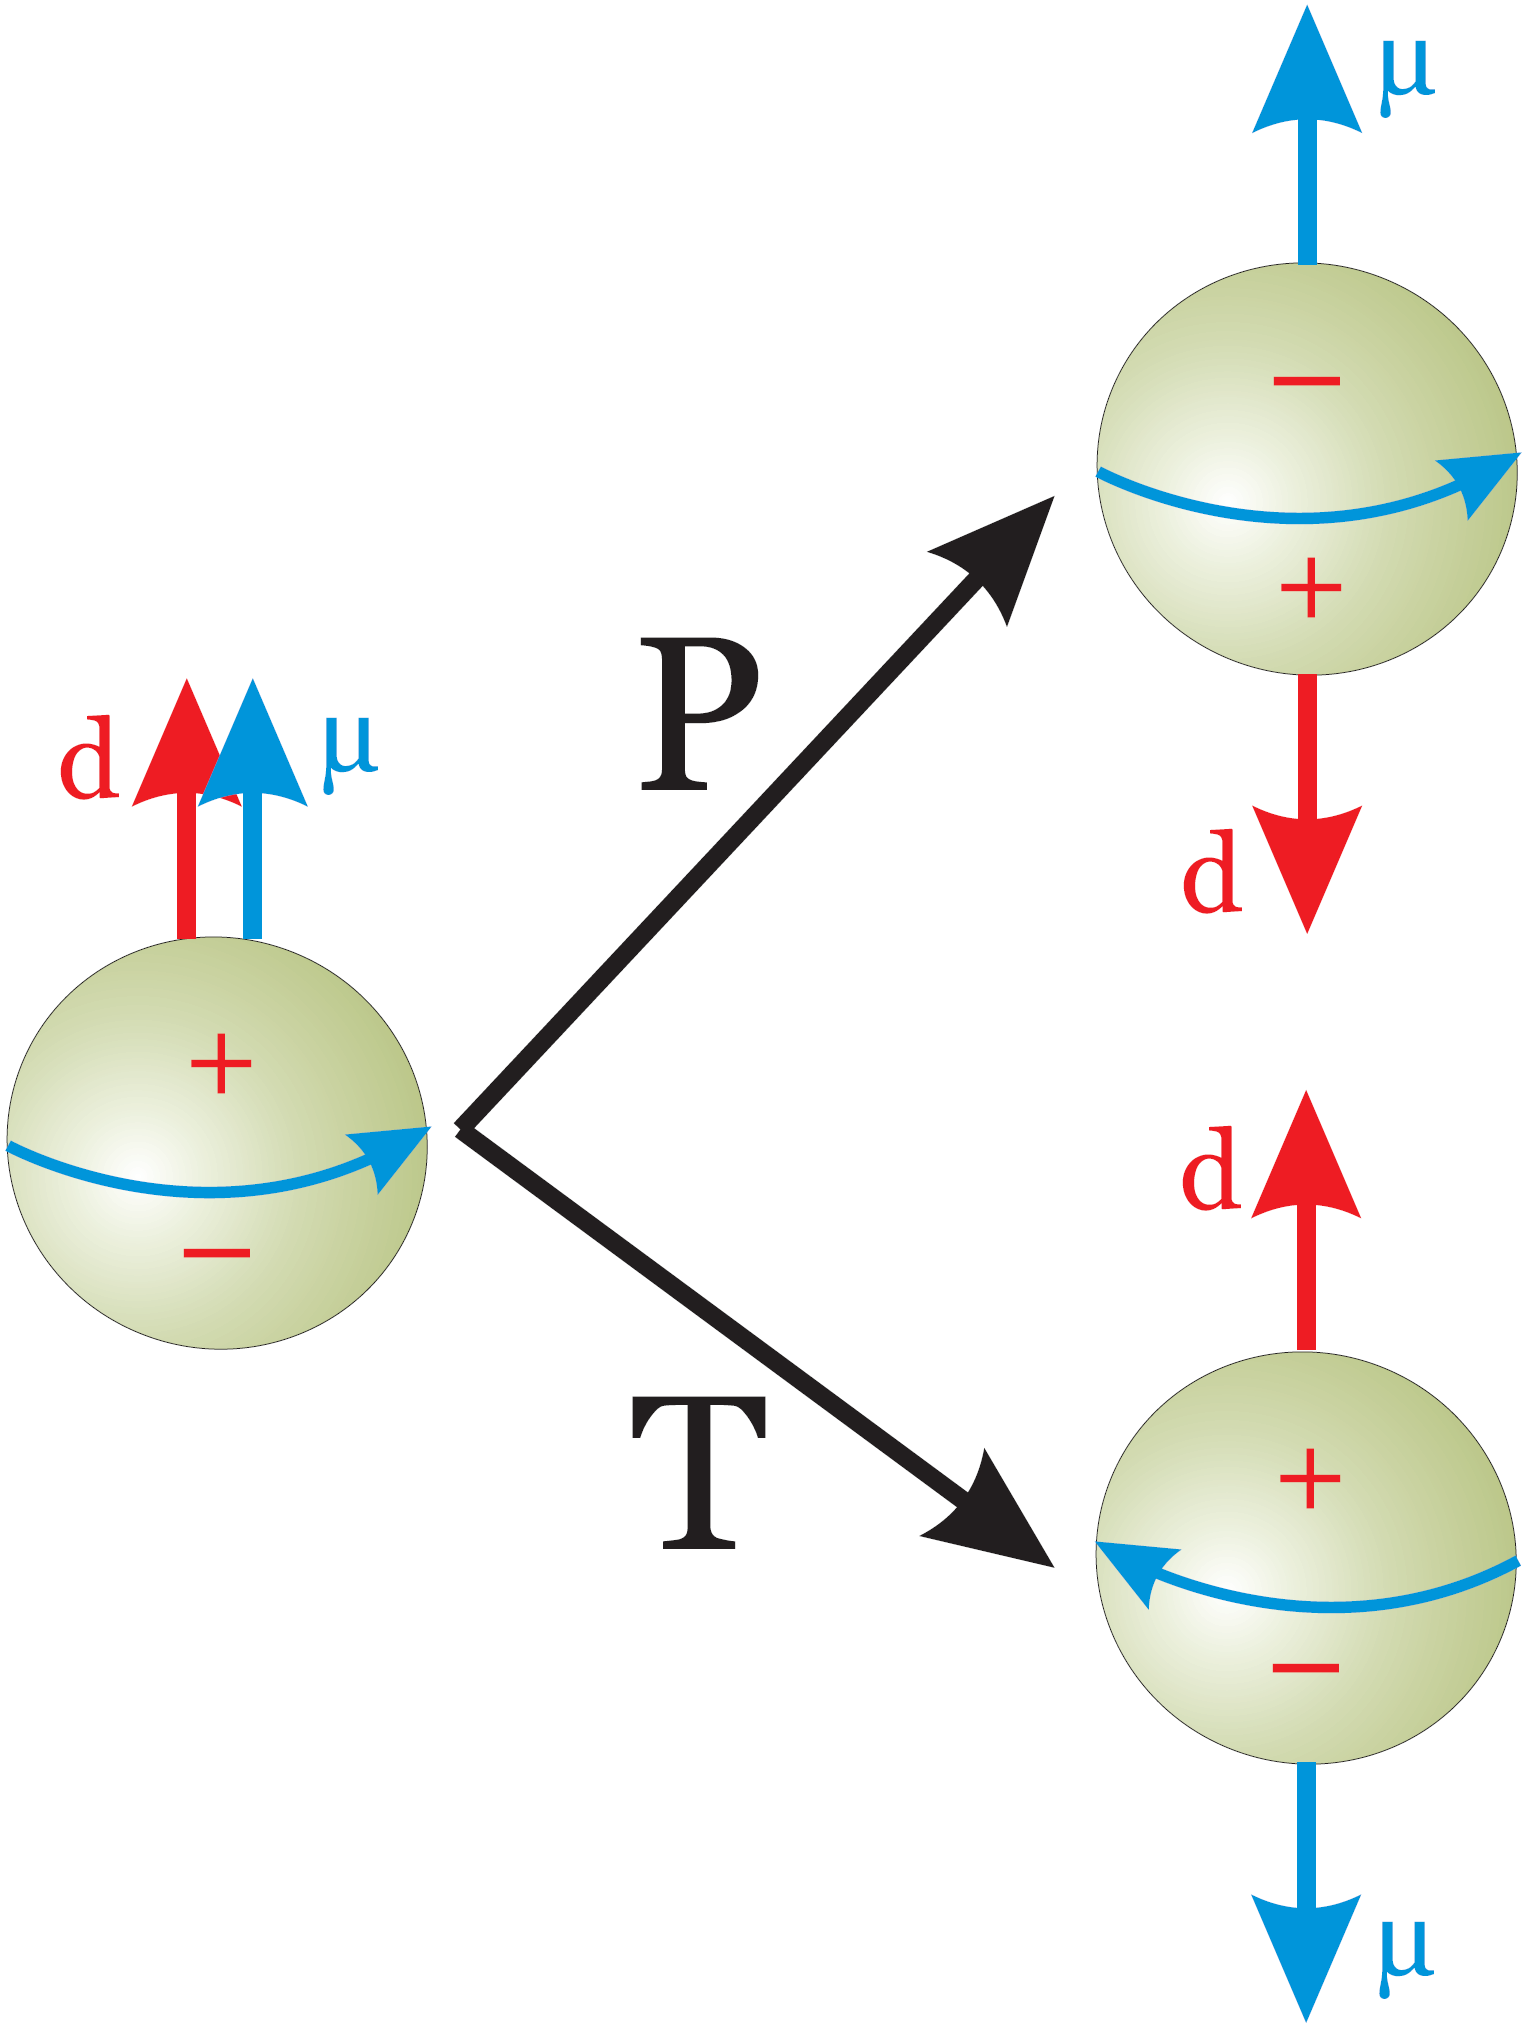
\includegraphics[width=0.4\linewidth]{images/4_EDM_P_T}
	\caption{Схематическое изображение нарушение P- и Т-симметрии ненулевым электрическим дипольным моментом.}
	\label{fig:4edmpt}
\end{figure}

\par	Исследование ЭДМ осуществляется согласно уравнению Т-БМТ по его влиянию на поведение поляризации в электромагнитных полях. В случае ЭДМ нейтрона, а также нейтральных атомов их положение сохраняется при действии внешних магнитных и электрических полей. В случае заряженных частиц происходит движение согласно силе Лоренца, что и приводит к необходимости применения ускорительных установок, позволяющих длительное накопление пучка с заданными параметрами и выступающих в роли накопительного кольца. Наиболее интересным и перспективным направлением выглядит изучение ЭДМ протона и дейтрона. Для этого требуется создание когерентных пучков. Тогда сохраняется поляризация вдоль конкретной оси, а также спины частиц прецессируют с одинаковой частотой. Для накопления малой величины ЭДМ необходимо долгое удержание пучка с последующим анализом рассеяния на мишени поляриметра. При этом влияние магнитного дипольного момента (МДМ) должно быть подавлено. Такая техника впервые была предложена в БНЛ (Брукхейвенская Национальная Лаборатория) и имеет название 'замороженный' спин \cite{Farley:edm}. Позднее, была предложена концепция 'квази-замороженного' спина \cite{QFS}, в которой происходит пространственное разделение полей и интегральное подавление МДМ-компоненты за полный оборот по кольцу.

\par	Ещё одним перспективным направлением исследований в рамках программы спиновой физики является исследование аксиона. В этом случае резонансным методом между частотой спиновой прецессии и частотой осциллирующего скалярного аксионового поля может быть получена масса аксиона или установлены соответствующие ограничения. Для этого ускоритель будет использован в роли зондирующей антенны по частоте прецессии спина \cite{Axion_Nikolaev}.

\par	Приведённые вопросы фундаментальной физики подлежат детальному рассмотрению и могут быть исследованы с использованием ускорительных установок, предназначенных для проведения разнообразных экспериментов. Эти установки позволяют достигать высоких энергий частиц, а также предельных точностей измерений. Такая практика применяется в крупных мировых ядерных центрах: CERN \cite{lhc:heavy_ions}, BNL \cite{rhic:design}, J-PARC \cite{j-park}. Последовательные программы экспериментов расписаны на годы и десятилетия вперед. В первую очередь такие установки служат для фундаментальных исследований, но также поддерживают широкий спектр прикладных задач в таких областях, как медицина, материаловедение и информационные технологии. Кроме того, ускорительные комплексы способствуют развитию необходимых технологий, что укрепляет научно-техническую базу и формирует долгосрочные положительные эффекты. Они также служат важной образовательной платформой, формируя программы для обучения молодых специалистов и предоставляют уникальные возможности для их профессионального роста. 

\par	Ускорительный комплекс NICA (Nuclotron-based Ion Collider fAсility) является современным передовым центром, который оборудован передовой материально-технической базой, отвечающей мировым тенденциям и формируется на базе ОИЯИ в городе Дубна, Россия \cite{nuclotron24}. Основной установкой комплекса является коллайдер, в котором предусмотрены два места встречи пучков, где расположены два детектора: MPD (Multi-Purpose Detector) и SPD (Spin Physics Detector) \cite{Ladygin:SPD}. Каждый из этих детекторов предназначен для различных экспериментов. MPD-детектор будет использован для исследования кварк-глюонной плазмы, возникающей в результате столкновения тяжёлых ионов \cite{MPD, Tech_NICA}. SPD-детектор направлен на изучение поведения сталкивающихся поляризованных пучков протонов и дейтронов. Кинематическая область, охватываемая SPD, уникальна и никогда не использовалась целенаправленно при поляризованных адронных столкновениях. Кроме того, уникальной возможностью станет изучение поляризованных дейтронов. Таким образом, структура коллайдера должна поддерживать ускорение как тяжёлых ионов, так и лёгких частиц. При этом требования к удержанию пучков для различных типов частиц существенно отличаются.

~\\
\par {\actuality} Исследования направлены на формирование полноценной физической программы по изучению динамики поляризованных пучков в комплексе Nuclotron-NICA. Применение изложенных в работе подходов возможно и на других похожих установках без потери общности.
~\\
\par {\aim} данной диссертации является изучение особенностей динамики лёгких поляризованных пучков для проведения коллайдерных экспериментов в дуальной структуре, а также исследования электрического дипольного момента с использованием квази-замороженной концепции.
Для достижения поставленной цели необходимо было 
решить следующие {\tasks}:
\begin{enumerate}[beginpenalty=10000] % https://tex.stackexchange.com/a/476052/104425
	\item	Определение требований к дуальной структуре для тяжелых ионов;
	\item	Регулирование критической энергии для поляризованных частиц методом резонансной модуляции дисперсионной функции;
	\item	Проведение численного моделирования динамики пучка легких частиц с учетом высших порядков коэффициента уплотнения орбиты в высокочастотых резонаторах гармонического и барьерного типа;
	\item 	Поведение динамической апертуры с учетом высших порядков при прохождении пучка через критическую энергию с скомпенсированной хроматичностью;
	\item 	Особенности поведения поляризации пучка при совершении процедуры скачка критической энергии;
	\item 	Изучение концепции «квази-замороженного» спина с целью создания установки для исследования ЭДМ дейтрона и протона;
	\item	Исследование спин-орбитального движения поляризованного пучка в магнитном кольце с фильтрами Вина;
\end{enumerate}
\begin{comment}
\begin{enumerate}[beginpenalty=10000] % https://tex.stackexchange.com/a/476052/104425
  \item Расчёт времени внутрипучкового рассеяния для тяжелых ионов;
  \item Оценка влияния методов с стохастического охлаждения пучка на время жизни;
  \item Моделирование магнитооптики с модулированной дисперсионной функцией;
  \item Проведение численного моделирования продольной динамики частиц с учетом высших порядков коэффициента уплотнения орбиты в высокочастотых резонаторах гармонического и барьерного типа;
  \item Обеспечение стабильности пучка с точки зрения динамической апертуры при процедуре скачка критической энергии, подавление хроматичности, компенсация нелинейных эффектов;
  \item Сохранение поляризации пучка при совершении процедуры скачка критической энергии;
  \item Изучение концепции «квази-замороженного» спина с целью создания установки для исследования ЭДМ дейтрона и протона;
  \item Спин-орбитальное моделирование в магнитном кольце с дополнительными элементами со скрещенными магнитными и электрическими полями;
\end{enumerate}
\end{comment}
~\\
\par {\novelty}
\begin{enumerate}[beginpenalty=10000] % https://tex.stackexchange.com/a/476052/104425
	\item	Впервые предложена дуальная структура для тяжелых ионов и легких частиц для коллайдера NICA;
	\item 	Впервые предложены методы подавления дисперсии поворотной аркой в резонансной магнитооптической структуре с отсутствующими магнитами;
	\item 	Впервые исследован метод скачка критической энергии с использованием барьерного ускоряющего потенциала с учётом ограничений по продольной микроволновой неустойчивости;
	\item	Были проведены исследования продольной динамики с учётом высших порядков разложения по импульсу, а также влиянием импеданса. На их базе сформулированы ограничения на величину и темп скачка критической энергии;
	\item	Были разработаны 8- и 16-периодичная квази-замороженная структура Nuclotron для выделения ЭДМ сигнала легких ядер;
	\item	Была разработана структура коллайдера NICA с обводными каналами, неориентированная изначально на эксперименты по поиску ЭДМ дейтрона методом квази-замороженного спина;
\end{enumerate}
\begin{comment}
	\item	Исследованы закономерности динамики многозарядных тяжёлых ионов и лёгких поляризованных частиц в дуальной магнитооптической структуре с учётом различий во внутрипучковом рассеянии и влияния критической энергии на устойчивость пучка;
 	\item 	Предложен метод резонансной модуляции дисперсионной функции с применением дополнительного семейства квадрупольных линз, что позволило повысить критическую энергию и стабильность пучка в режиме ускорения лёгких частиц;
 	\item	Приведены способы подавления дисперсии на краях поворотных арок в отсутствии регулярности, а также способы подавления нелинейных эффектов;
 	\item 	Выполнено численное моделирование прохождения критической энергии с учётом высших порядков зависимости от импульсного разброса, а также влияния импедансов, что позволило количественно оценить влияние данных факторов на сохранение пучка;
 	\item	Исследована продольная динамика поляризованного пучка при нахождении вблизи и прохождении критической энергии методом скачка в гармоническом и барьерном ВЧ, что позволило количественно оценить стабильность пучка в различных режимах ускорения;
 	\item	Предложено применение метода фильтров Вина для сохранения направления поляризации в пучках, что расширяет возможности по исследованию электрического дипольного момента и аксионоподобных частиц;
 	\item	Рассмотрены вариации изучения ЭДМ дейтрона и протона в много-периодичных структурах с использованием электростатических дефлекторов или фильтров Вина;
\end{comment}
~\\
\par {\influence}:
\par Исследование динамики пучка вблизи критической энергии показывает необходимость её преодоления, а также  способствует определению оптимальных параметров скачка критической энергии. Определено существенное влияние критической энергии на динамику поляризованного протонного пучка.

\par В качестве решения проблем с тяжелыми и легкими частицами разработана дуальная структура. Дуальность структуры указывает на возможность её эффективного решения обоих эффектов и использования сразу для двух фундаментально значимых исследований: для изучения кварк-глюонной плазмы в коллайдерных экспериментах с тяжелыми ионами и для исследования легких поляризованных пучков в симметричных и асимметричных коллайдерных столкновениях.

\par Расширена применимость метода «резонансных структур» для случая отсутствия периодичности дисперсионной функции на арках.

\par В части поляризованных частиц адаптирован метод “квази-замороженного спина” для коллайдера NICA, продемонстрировавший возможность проведения исследований по электрическому дипольному моменту без значительных изменений структуры ускорителя. Разработана магнитооптическая структура обводных каналов bypass, позволяющая обойти точки встречи для обоих детекторов с расположенными на них прямыми фильтрами Вина. Данная схема позволяет реализовать концепцию "квази-замороженного спина" для исследования электрического дипольного момента дейтрона. 

\par Методы разработанные для кольца NICA могут быть использованы и для Nuclotron с сохранением функций бустера для поляризованного пучка в коллайдер. Это также позволит проведение независимых экспериментов по исследованию ЭДМ и поиску аксиона. Такие исследования является отдельной частью программы спиновой физики, которая формируется на уста­новке NICA-Nuclotron.


% {\progress}
% Этот раздел должен быть отдельным структурным элементом по
% ГОСТ, но он, как правило, включается в описание актуальности
% темы. Нужен он отдельным структурынм элемементом или нет ---
% смотрите другие диссертации вашего совета, скорее всего не нужен.
~\\
\par {\methods} Основными методами исследования являются математическое и компьютерное моделирование, численный эксперимент. Для исследования были использованы программы для расчёта поперечной динамики: MAD-X \cite{madx}, OPTIM \cite{optim}, BMAD \cite{bmad}, продольной динамики: BLonD \cite{blond}; спин-орбитальной динамики: COSY Infinity \cite{cosy}.
~\\
%второй вариант
\begin{comment}
\par {\defpositions}
\begin{enumerate}[beginpenalty=10000] % https://tex.stackexchange.com/a/476052/104425
  \item 	Принципы построения дуальной магнитооптической структуры с оптимизированным временем жизни пучка в регулярной структуре для многозарядных тяжелых ионов и варьированной критической энергией в резонансной структуре для легких ядер; \cite{Kolokolchikov:2025_dual}, \cite{Syresin:2021_polar}
  \item	Результаты, полученные в эксперименте на У-70 и в методе численного моделирования динамики продольного движения вблизи критической энергии с учётом влияния высших порядков зависимости от разброса по импульсу и с учетом импеданса; \cite{Kolokolchikov:2025_U70}, \cite{Kolokolchikov:2025_jump}
  \item	Результаты исследования продольной динамики поляризованного пучка для процедуры скачка критической энергии в гармоническом и барьерном ВЧ, оценка влияния продольной микроволновой неустойчивости; \cite{Kolokolchikov:2024_bb_rupac}, \cite{Kolokolchikov:2023_bb_IPAC}, \cite{Kolokolchikov:2024_bb_dspin}
  \item	Метод подавления дисперсии и влияния нелинейных эффектов, из-за нарушения периодичности за счет введения missing magnet на краях поворотных арок, для создания резонансной магнитооптической структуры; \cite{Kolokolchikov:2021trans}, \cite{Kolokolchikov:2023_pecular}
  \item	Модернизированная структура с квази-замороженным спином для исследования ЭДМ дейтронов и протонов и возможностью совместного использования Нуклотрона в качестве бустера поляризованных частиц для коллайдера; \cite{Senichev:2023_QFS}, \cite{Senichev:2023_nuclotron}, \cite{Kolokolchikov:2025_nuclotron}
  \item	Метод обводных каналов bypass для независимого исследования ЭДМ в кольце коллайдера;\cite{Kolokolchikov:2023_bypass}, \cite{Kolokolchikov:2023_bypass_IPAC}, \cite{Senichev:2024_nica_edm}, \cite{Kolokolchikov:2023_sc}, \cite{Kolokolchikov:2023_sc_IPAC}
\end{enumerate}
\end{comment}

%третий вариант
\begin{comment}
\par {\defpositions}
\begin{enumerate}[beginpenalty=10000] % https://tex.stackexchange.com/a/476052/104425
  \item 	Изучение внутрипучкового рассеяния и стохастического охлаждения для оптимизации времени жизни пучка в регулярной структуре для многозарядных тяжелых ионов и варьированной критической энергией в резонансной структуре для легких ядер с целью реализации дуальности ускорительной установки; \cite{Kolokolchikov:2025_dual}, \cite{Syresin:2021_polar}
  \item	Результаты, полученные в эксперименте на У-70 и в методе численного моделирования динамики продольного движения вблизи критической энергии с учётом влияния высших порядков зависимости от разброса по импульсу и с учетом импеданса; \cite{Kolokolchikov:2025_U70}, \cite{Kolokolchikov:2025_jump}
  \item	Результаты исследования продольной динамики поляризованного пучка для процедуры скачка критической энергии в гармоническом и барьерном ВЧ, оценка влияния продольной микроволновой неустойчивости; \cite{Kolokolchikov:2024_bb_rupac}, \cite{Kolokolchikov:2023_bb_IPAC}, \cite{Kolokolchikov:2024_bb_dspin}
  \item	Метод подавления дисперсии и влияния нелинейных эффектов в резонансной магнитооптической структуре из-за нарушения периодичности по дисперсии за счет missing magnet на краях поворотных арок; \cite{Kolokolchikov:2021trans}, \cite{Kolokolchikov:2023_pecular}
  \item	Модернизированная структура с квази-замороженным спином для исследования ЭДМ дейтронов и протонов и возможностью совместного использования Нуклотрона в качестве бустера поляризованных частиц для коллайдера; \cite{Senichev:2023_QFS}, \cite{Senichev:2023_nuclotron}, \cite{Kolokolchikov:2025_nuclotron}
  \item	Метод введения обводных каналов в кольцо синхротрона для создания независимой установки с возможностью проведения прецизионных экспериментов, в том числе изучения ЭДМ элементарных частиц;\cite{Kolokolchikov:2023_bypass}, \cite{Kolokolchikov:2023_bypass_IPAC}, \cite{Senichev:2024_nica_edm}, \cite{Kolokolchikov:2023_sc}, \cite{Kolokolchikov:2023_sc_IPAC}
\end{enumerate}
\end{comment}

\begin{comment}
\par {\defpositions}
\begin{enumerate}[beginpenalty=10000] % https://tex.stackexchange.com/a/476052/104425
  \item 	Основные свойства дуальной магнитооптической структуры для легких ядер и тяжелых частиц с учетом различия внутрипучкового рассеяния. Время жизни пучка в дуальной структуре с учетом вариации коэффициента проскальзывания в разных арках; \cite{Kolokolchikov:2025_dual}, \cite{Syresin:2021_polar}
  \item	Учет влияния высших порядков разброса по импульсам и моделей продольных импедансов в численном моделировании движения в окрестности критической энергии и сравнение с экспериментальными результатами, полученными на У-70; \cite{Kolokolchikov:2025_U70}, \cite{Kolokolchikov:2025_jump}
  \item	Результаты математического моделирования процесса прохождения ансамбля частиц через критическую энергию с различной скоростью и при различной форме ускоряющего потенциала с учетом ограничений по продольной микроволновой неустойчивости; \cite{Kolokolchikov:2024_bb_rupac}, \cite{Kolokolchikov:2023_bb_IPAC}, \cite{Kolokolchikov:2024_bb_dspin}
  \item	Резонансная модуляция дисперсионной функции, как метод вариации критической энергии. Результаты оптимизации дисперсионной функции при наличии отсутствующих магнитов (missing magnets); \cite{Kolokolchikov:2021trans}, \cite{Kolokolchikov:2023_pecular}
  \item	Особенности поляризованных пучков, используемых для исследования электрического дипольного момента в структурах с квази-замороженным спином на примере модернизированной структуры Нуклотрона; \cite{Senichev:2023_QFS}, \cite{Senichev:2023_nuclotron}, \cite{Kolokolchikov:2025_nuclotron}
  \item	Метод фильтров Вина для сохранении направления поляризации  на основе введения обводных каналов в структуре с квази-замороженным спином для выделения ЭДМ сигнала в поляризованном пучке;\cite{Kolokolchikov:2023_bypass}, \cite{Kolokolchikov:2023_bypass_IPAC}, \cite{Senichev:2024_nica_edm}, \cite{Kolokolchikov:2023_sc}, \cite{Kolokolchikov:2023_sc_IPAC}
\end{enumerate}
\end{comment}

\par {\defpositions}
\begin{enumerate}[beginpenalty=10000] % https://tex.stackexchange.com/a/476052/104425
	\item 	Предложена реализация дуальной структуры для комплекса NICA-Nuclotron, оптимальная для тяжелых частиц с точки зрения внутрипучкового рассеяния и легких частиц с поднятой критической энергией выше энергии эксперимента; \cite{Kolokolchikov:2025_dual, Syresin:2021_polar}
	\item	Реализован метод вариации критической энергии для магнитооптики коллайдера NICA с отсутствующими магнитами при подавлении дисперсионной функции двумя семействами квадруполей и двумя крайними ячейками поворотной арки; \cite{Kolokolchikov:2021trans, Kolokolchikov:2023_pecular}
	\item	Представлены результаты численного моделирования продольной динамики с учетом влияния высших порядков разброса по импульсам и моделей продольных импедансов в окрестности критической энергии и сравнение с экспериментальными результатами, полученными на У-70; \cite{Kolokolchikov:2025_U70, Kolokolchikov:2025_jump}
	\item 	Проведен анализ использования гармонического ВЧ при процедуре скачка в коллайдере NICA. Для барьерного ВЧ представлены данные моделирования продольной динамики, а также предложено сокращение длины между барьерами из-за продольной микроволновой неустойчивости; \cite{Kolokolchikov:2024_bb_rupac, Kolokolchikov:2023_bb_IPAC, Kolokolchikov:2024_bb_dspin}
	\item	Предложены модернизированные квази-замороженные 8/16-периодичные структуры Nuclotron для исследования электрического дипольного момента легких ядер, с сохранением функции бустера. \cite{Senichev:2023_QFS, Senichev:2023_nuclotron, Kolokolchikov:2025_nuclotron}
	\item	Применен метод фильтров Вина для сохранении направления поляризации на основе введения обводных каналов в структуре коллайдера NICA с квази-замороженным спином для выделения ЭДМ сигнала в поляризованном пучке дейтронов;\cite{Kolokolchikov:2023_bypass, Kolokolchikov:2023_bypass_IPAC, Senichev:2024_nica_edm, Kolokolchikov:2023_sc, Kolokolchikov:2023_sc_IPAC}
\end{enumerate}

~\\
\par {\reliability} полученных результатов подтверждается согласованием аналитических вычислений с результатами численных экспериментов. Результаты находятся в соответствии с результатами, полученными другими авторами.
~\\
\par {\probation}
Основные результаты работы были представлены докладывались~на российских и международных конференциях, а также рабочих встречах: 
\begin{itemize}
\item Workshop “Polarized beam in NICA” в 2022 г.;
\item Молодежная конференция по теоретической и экспериментальной физике МКТЭФ-2020. Москва, Россия;
\item 63, 65, 66-ая Всероссийская научная конференция МФТИ в 2020, 2023, 2024 гг. г. Долгопрудный,
Россия;
\item XXVII и XXVIII Всероссийская конференции по ускорителям заряженных частиц RuPAC'21, RuPAC'23. Алушта; Новосибирск, Россия.
\item VII, VIII, IX и X Международная конференция Лазерные и Плазменные технологии ЛаПлаз'21, ЛаПлаз'22, ЛаПлаз'23, ЛаПлаз'24, ЛаПлас'25. Москва, Россия;
\item XIII, XIV, XVI международная конференция по ускорителям заряженных частиц IPAC'22 IPAC'23, IPAC'25. Бангкок, Тайланд; Венеция, Италия; Тайпей, Тайвань;
\item XIX Международная конференции по спиновой физике высоких энергий DSPIN'23. Дубна, Россия;
\item XI-я Международная конференция по ядерной физике в накопительных кольцах STORI’24. Хуэйчжоу, провинция Гуандун, Китай;
\end{itemize}
~\\
\par {\contribution} Все результаты, выносимые на защиту, получены автором лично, либо при его непосредственном участии. Содержание диссертации и выносимые на защиту основные положения отражают личный вклад автора в опубликованные работы. Результаты по подготовке и проведению эксперимента на ускорителе У-70 получены в соавторстве с сотрудниками ИЯИ РАН и ИФВЭ. Подготовка к публикации полученных результатов проводилась совместно с соавторами.
~\\
\par \ifnumequal{\value{bibliosel}}{0}
{%%% Встроенная реализация с загрузкой файла через движок bibtex8. (При желании, внутри можно использовать обычные ссылки, наподобие `\cite{vakbib1,vakbib2}`).
 {\publications} Основные результаты по теме диссертации изложены
    в~XX~печатных изданиях,
    X из которых изданы в журналах, рекомендованных ВАК,
    X "--- в тезисах докладов.
}%
{%%% Реализация пакетом biblatex через движок biber
    \begin{refsection}[bl-author, bl-registered]
        % Это refsection=1.
        % Процитированные здесь работы:
        %  * подсчитываются, для автоматического составления фразы "Основные результаты ..."
        %  * попадают в авторскую библиографию, при usefootcite==0 и стиле `\insertbiblioauthor` или `\insertbiblioauthorgrouped`
        %  * нумеруются там в зависимости от порядка команд `\printbibliography` в этом разделе.
        %  * при использовании `\insertbiblioauthorgrouped`, порядок команд `\printbibliography` в нём должен быть тем же (см. biblio/biblatex.tex)
        %
        % Невидимый библиографический список для подсчёта количества публикаций:
        \printbibliography[heading=nobibheading, section=1, env=countauthorvak,          keyword=biblioauthorvak]%
        \printbibliography[heading=nobibheading, section=1, env=countauthorwos,          keyword=biblioauthorwos]%
        \printbibliography[heading=nobibheading, section=1, env=countauthorscopus,       keyword=biblioauthorscopus]%
        \printbibliography[heading=nobibheading, section=1, env=countauthorconf,         keyword=biblioauthorconf]%
        \printbibliography[heading=nobibheading, section=1, env=countauthorother,        keyword=biblioauthorother]%
        \printbibliography[heading=nobibheading, section=1, env=countregistered,         keyword=biblioregistered]%
        \printbibliography[heading=nobibheading, section=1, env=countauthorpatent,       keyword=biblioauthorpatent]%
        \printbibliography[heading=nobibheading, section=1, env=countauthorprogram,      keyword=biblioauthorprogram]%
        \printbibliography[heading=nobibheading, section=1, env=countauthor,             keyword=biblioauthor]%
        \printbibliography[heading=nobibheading, section=1, env=countauthorvakscopuswos, filter=vakscopuswos]%
        \printbibliography[heading=nobibheading, section=1, env=countauthorscopuswos,    filter=scopuswos]%
        %
        \nocite{*}%
        %
        {\publications} Основные результаты по теме диссертации изложены в~\arabic{citeauthor}~печатных изданиях,
        \arabic{citeauthorvak} из которых изданы в журналах, рекомендованных ВАК\sloppy%
        \ifnum \value{citeauthorscopuswos}>0%
            , \arabic{citeauthorscopuswos} "--- в~периодических научных журналах, индексируемых Web of~Science и Scopus\sloppy%
        \fi%
        \ifnum \value{citeauthorconf}>0%
            , \arabic{citeauthorconf} "--- в~тезисах докладов.
        \else%
            .
        \fi%
        \ifnum \value{citeregistered}=1%
            \ifnum \value{citeauthorpatent}=1%
                Зарегистрирован \arabic{citeauthorpatent} патент.
            \fi%
            \ifnum \value{citeauthorprogram}=1%
                Зарегистрирована \arabic{citeauthorprogram} программа для ЭВМ.
            \fi%
        \fi%
        \ifnum \value{citeregistered}>1%
            Зарегистрированы\ %
            \ifnum \value{citeauthorpatent}>0%
            \formbytotal{citeauthorpatent}{патент}{}{а}{}\sloppy%
            \ifnum \value{citeauthorprogram}=0 . \else \ и~\fi%
            \fi%
            \ifnum \value{citeauthorprogram}>0%
            \formbytotal{citeauthorprogram}{программ}{а}{ы}{} для ЭВМ.
            \fi%
        \fi%
        % К публикациям, в которых излагаются основные научные результаты диссертации на соискание учёной
        % степени, в рецензируемых изданиях приравниваются патенты на изобретения, патенты (свидетельства) на
        % полезную модель, патенты на промышленный образец, патенты на селекционные достижения, свидетельства
        % на программу для электронных вычислительных машин, базу данных, топологию интегральных микросхем,
        % зарегистрированные в установленном порядке.(в ред. Постановления Правительства РФ от 21.04.2016 N 335)
    \end{refsection}%
    \begin{refsection}[bl-author, bl-registered]
        % Это refsection=2.
        % Процитированные здесь работы:
        %  * попадают в авторскую библиографию, при usefootcite==0 и стиле `\insertbiblioauthorimportant`.
        %  * ни на что не влияют в противном случае
        \nocite{vakbib2}%vak
        \nocite{patbib1}%patent
        \nocite{progbib1}%program
        \nocite{bib1}%other
        \nocite{confbib1}%conf
    \end{refsection}%
        %
        % Всё, что вне этих двух refsection, это refsection=0,
        %  * для диссертации - это нормальные ссылки, попадающие в обычную библиографию
        %  * для автореферата:
        %     * при usefootcite==0, ссылка корректно сработает только для источника из `external.bib`. Для своих работ --- напечатает "[0]" (и даже Warning не вылезет).
        %     * при usefootcite==1, ссылка сработает нормально. В авторской библиографии будут только процитированные в refsection=0 работы.
}


 % Характеристика работы по структуре во введении и в автореферате не отличается (ГОСТ Р 7.0.11, пункты 5.3.1 и 9.2.1), потому её загружаем из одного и того же внешнего файла, предварительно задав форму выделения некоторым параметрам

\textbf{Объем и структура работы.} Диссертация состоит из~введения,
\formbytotal{totalchapter}{глав}{ы}{}{}
и заключения.
%и \formbytotal{totalappendix}{приложен}{ия}{ий}{}.
%% на случай ошибок оставляю исходный кусок на месте, закомментированным
%Полный объём диссертации составляет  \ref*{TotPages}~страницу
%с~\totalfigures{}~рисунками и~\totaltables{}~таблицами. Список литературы
%содержит \total{citenum}~наименований.
%
Полный объём диссертации составляет
\formbytotal{TotPages}{страниц}{у}{ы}{}, включая
\formbytotal{totalcount@figure}{рисун}{ок}{ка}{ков} и
\formbytotal{totalcount@table}{таблиц}{у}{ы}{}.
Список литературы содержит
\formbytotal{citenum}{наименован}{ие}{ия}{ий}.

В \textbf{первой} главе особое внимание уделено процессам внутрипучкового рассеяния и роли критической энергии, влияющим на динамику многозарядных тяжёлых ионов и лёгких ядер. С этой целью рассматривается дуальная магнитооптическая структура, адаптируемая для обоих типов экспериментов.

\par Для тяжёлых ионов ключевым фактором становится внутрипучковое рассеяние. Разогрев пучка приводит к росту поперечного эмиттанса и продольного разброса по импульсам. Для стабилизации параметров используются методы электронного и стохастического охлаждения.

\par В случае лёгких частиц, таких как протоны, соотношение заряда к массе примерно в два раза выше, чем у тяжёлых ионов, что пропорционально повышает энергию эксперимента. При этом критическая энергия остаётся неизменной, поскольку определяется магнитооптической структурой установки. Для устойчивого продольного движения необходимо её преодоление. Одним из эффективных способов является применение резонансной структуры для повышения критической энергии.

\par Во \textbf{второй} главе рассмотрено влияние высших порядков разброса по импульсам и продольных импедансов при пересечении критической энергии, а также метод скачка критической энергии для различных ускоряющих потенциалов.

\par Продольная микроволновая неустойчивость вблизи критической энергии накладывает ограничения на параметры сгустка и светимость эксперимента. Для преодоления критической энергии классически используется процедура скачка критической энергии. Данная процедура осуществляется модулированием дисперсионной функции при приближении энергии пучка к критическому значению. Результаты численного моделирования сопоставлены с экспериментами на ускорителе У-70 (Протвино). Также проанализировано влияние высших порядков расширения орбиты и простейших моделей импедансов на динамику пучка.

\par В \textbf{третьей} главе рассматривается вариация критической энергии в резонансной структуре. Для этого используется суперпериодическая модуляция градиентов квадрупольных линз или модуляция кривизны орбиты, что приводит к изменению коэффициента уплотнения орбиты — величины, напрямую связанной с критической энергией ускорителя.

\par Для регулярной магнитооптической структуры коллайдера NICA проанализированы варианты модернизации, позволяющие повысить критическую энергию. Поскольку установка является стационарной, реализация резонансной структуры возможна за счёт модуляции градиентов в квадрупольных линзах. Для полученных конфигураций представлены схемы размещения секступолей.

В \textbf{четвёртой} главе рассматривается возможность изучения электрического дипольного момента лёгких заряженных частиц. Исследована концепция квази-замороженного спина для накопительных колец, позволяющая модернизировать кольца без изменения их базового назначения и расширить экспериментальные возможности. Проанализирована спиновая динамика в кольце с использованием электростатических элементов и элементов с комбинированной функцией.

\par Для экспериментов по поиску ЭДМ применяется альтернативный метод управления спином — квази-замороженный спин. В отличие от метода замороженного спина, спин-вектор не сохраняет ориентацию на всём обороте, а восстанавливается на прямолинейном участке. Это достигается использованием элементов с электрическим и магнитным полями — электростатического дефлектора с магнитным киккером или фильтра Вина. Поворот спина в арке компенсируется соответствующим поворотом в компенсирующем элементе. Поля подбираются так, чтобы создать нулевую силу Лоренца и сохранить прямолинейность орбиты. Поляриметры после компенсации фиксируют ту же ориентацию спин-вектора, которая для них оказывается «замороженной».

В \textbf{заключении} приведены результаты работы.    % Введение
\ifnumequal{\value{contnumfig}}{1}{\counterwithout{figure}{chapter}
}{\counterwithin{figure}{chapter}}
\ifnumequal{\value{contnumtab}}{1}{\counterwithout{table}{chapter}
}{\counterwithin{table}{chapter}}
%part 1

\chapter{Особенности двойственной магнитооптической структуры коллайдера NICA для ускорения тяжелых ионов и легких частиц частиц}\label{ch:ions_light}

\section{Дуальность магнитооптической структуры NICA для тяжелых ионов и легких ядер}\label{sec:ch:ions_light/duality}

\section{Выбор критической энергии в магнитооптической структуре с учетом ускорения тяжелых ионов и легких частиц.}\label{sec:ch:ions_light/transition}

\subsection{Критическая энергия}\label{sec:ch:ions_light/transition/energy}
\par Понятие критическая энергия одно из ключевых в данной работе, поэтому уделим внимание к его определению. 
\par Рассмотрим классическое уравнение продольного движение, описывающее эволюцию частицы отклоненной от референсной:

\begin{equation}
\begin{aligned}
& \frac{d \tau}{d t}=\eta(\delta) \cdot \frac{h \cdot \Delta E}{\beta^2 \cdot E_0} \\
& \frac{d(\Delta E)}{d t}=\frac{V(\tau)}{T_0}
\end{aligned}
\label{eq:long_motion_eq}
\end{equation}

\noindent где $\tau$ – временное отклонение рассматриваемой частицы от референсной, $\beta$ – относительная скорость, $\omega_0=\sfrac{2\pi}{T_0}$– угловая частота и соответствующее время обращения, $h$ – гармоническое число, $V$ – ВЧ, $\eta$ коэффициент проскальзывания (в англоязычной терминологии 'slip-factor') 

\par При рассмотрении продольного движения вводится понятие коэф\-фи\-ци\-ента
расширения орбиты (momentum compaction factor) \cite{lee}:

\begin{equation}
\alpha_c=\frac{1}{R_0} \frac{d R}{d \delta}=\alpha_0+2 \alpha_1 \delta+3 \alpha_2 \delta^2+\cdots \equiv \frac{1}{\gamma_T^2}
\label{eq:alpha}
\end{equation}

и коэффициента скольжения (slip-factor):

\begin{equation}
\eta(\delta)=\eta_0+\eta_1 \delta+\eta_2 \delta^2+\cdots,
\label{eq:eta}
\end{equation}

\noindent где $\eta_0=\alpha_0-\frac{1}{\gamma_0^2}$, $\eta_1=\frac{3\beta_0^2}{2\gamma_0^2}+\alpha_1-\alpha_0\eta_0$.

\par В ур.\ref{eq:long_motion_eq}, если энергия пучка приближается к критической $\gamma\rightarrow\gamma_{tr},$  то $\eta=\eta_0\rightarrow0$, правая часть уравнения обращается в ноль. Возникает необходимость обеспечения стабильности при прохождении критической энергии.

\par критическая энергия 

\section{Решение проблемы внутрипучкового рассеяния для тяжелых ионов и протонов в ускорителе NICA }\label{sec:ions_light/IBS}

\section{IBS в «резонансной» и регулярной структурах}\label{sec:ions_light/IBS_res_reg}

\FloatBarrier
           % Глава 1
%part 2

	\chapter{Прохождение критической энергии в регулярной магнитооптической структуре синхротрона}\label{ch:transition}

\par Данная глава посвящена рассмотрению влияния критической энергии на продольную динамику, а также процедуры скачка критической энергии в регулярной структуре синхротрона. Учтены высшие порядки, а также рассмотрены модели импеданса для разных интенсивностей.

\par Исходя из изложенных уравнений продольного движения в Главе \ref{ch:dual}, приближение энергии пучка к критическому значению ведет к изохронному движению, при котором частота синхротронных колебаний стремится к нулю и означает отсутствие продольного перемешивания частиц в сепаратрисе. При этом нарушается адиабатичность движения а также проявляется влияние высших порядков зависимости от разброса по импульсу – нелинейность. При этом затухание Ландау оказывается неспособно подавить возникающие возмущения в интенсивных сгустках, а наличие пространственного заряда и других импедансов оказывает влияние на развитие продольной микроволновой неустойчивости, нестабильности отрицательной массы и поперечной голова-хвост (head-tail) \cite{ng}, \cite{MetralMohl} и в конечном счёте теряется фазовая стабильность.

\par Увеличение скорости прохождения критической энергии уменьшает влияние факторов, возмущающих фазовое движение. Широко используется метод скачка критической энергии, который применяется на многих установках CERN \cite{risselada:jump}, BNL \cite{ainsworth:pip}, в том числе был реализован в России на синхротроне У-70 \cite{pashkov:transition}. Сдвиг критической энергии обеспечивается искажением дисперсионной функции. Для этого могут быть использованы разные методы -- изменение частоты бетатронных колебаний в регулярной структуре, применение дополнительных квадруполей с обратной полярностью, расположенных через один период друг от друга. Указанные методы для каждой отдельной установки рассматривается отдельно и устанавливают ограничения в зависимости от потребностей конечного эксперимента.

\par Прохождение критической энергии является актуальной задачей для протонного пучка в строящемся комплексе NICA (ОИЯИ г. Дубна). С целью изучения данной проблемы, исследована динамика продольного движения в окрестности критической энергии У-70 (НИЦ “Курчатовский институт” - ИФВЭ г. Протвино).  Промоделирована процедура скачка критической энергией в синхротроне У-70 при помощи численного моделирования. Полученные данные также апробированы на ускорительном сеансе \cite{Kolokolchikov:2025_U70}.

\par Важным фактором, описывающим взаимодействие пучка и элементов ускорителя является влияние различного рода импедансов, а также типо высокочастотных резонаторов (ВЧ) на продольную динамику во время процедуры преодоления критической энергии. Отличительной особенностью является использование ВЧ барьерного типа, в результате чего достигается специфическое распределение пучка в фазовом пространстве, отличное от классического, формируемого гармоническим ВЧ \cite{hans:bb}.

\par Результаты данного исследования помогут осветить потенциальные последствия прохождения критической энергии и определить существенные параметры, влияющие на динамику фазового движения.

	\section{Построение регулярной структуры на основе ячеек ФОДО, ФДО, ОДФДО}\label{sec:transition_jump/FODO_FDO}



\begin{figure} [h!]

   \includegraphics*[width=.32\columnwidth]{2_twiss_fodo_cell.pdf}
   \includegraphics*[width=.32\columnwidth]{2_twiss_fdo_cell.pdf}
   \includegraphics*[width=.32\columnwidth]{2_twiss_odfdo_cell.pdf}

   \includegraphics*[width=.32\columnwidth]{2_twiss_fodo_regular.pdf}
   \includegraphics*[width=.32\columnwidth]{2_twiss_fdo_regular.pdf}
   \includegraphics*[width=.32\columnwidth]{2_twiss_odfdo_regular.pdf}

   \caption{Твисс-параметры $\beta_{x,y}$, $D_{x}$. Сверху -- для ячеек для сигнлетной ФОДО, дублетной ФДО, триплетной ОДФДО ячеек; посредине -- регулярная структура; снизу -- резонансная.}
   \label{fig:fodo_fdo_odfdo_regular}
\end{figure}

\par На основе ФОДО, ФДО и ОДФДО ячеек могут быть сконструированы регулярные поворотные арки как показано на рис. \ref{fig:fodo_fdo_odfdo_regular}. Для ФОДО ячейки характерно максимальное пространственное разделение минимумов и максимумов бета-функций. Однако, максимальное значение бета-функции и дисперсионной функции наибольшее для ФОДО структуры. Также стоит отметить, что растет градиент в квадрупольных линзах для постижения одинакового набега фазы, в следующем порядке: ФОДО, ФДО, ОДФДО. 

	\subsection{Подавление дисперсии в регулярных арках с missing magnet и/или квадруполями с варьируемыми градиентами}\label{sec:transition_jump/suppression}

\par Дисперсионная функция $D(s)$ является решением неоднородного уравнения поперечного движения.
И является показателем зависимости смещения замкнутой орбиты для вне осевых частиц с ненулевым разбросом по импульсу $\delta$ \cite{lee}.

\par Необходимость наличия бездисперсионных областей встречается в ряде задач в ускорительной технике. Для коллайдерных экспериментов, пучки сталкивается в определенной заданной точке (Interaction Point - IP) и для достижения большой светимости требуется в точке встречи иметь минимальный поперечный размер пучка, который пропорционален дисперсионной функции. Кроме того, при инжекции из бустера (buster) в основное кольцо (main ring), необходимо согласование Твисс-функций для сохранения пучка. Такое условие может легко достигаться в случае нулевой дисперсии. В обратом случае, необходимо нарочно возбуждать орбиту для их согласования. Также, установка определенных элементов, таких как высокочастотные резонаторы, в места нулевой дисперсии минимизирует эффект синхро-бетатронных резонансов связи.

\par Наиболее простым способом дисперсия в поворотной арке может быть подавлена в периодичной структуре, где частота кратна целому числу $2\pi$, при таком подходе создаётся ахромат первого порядка. Другим известным, уже ставшим классическим, является подход с введением техники 'отсутствующих' магнитов ('missing magnet') \cite{autin:dispersion}. В этом случае, не реализуются условия ахромата первого порядка. Так, в коллайдере NICA реализована техника отсутствующих магнитов и инжекция происходит в место с ненулевой дисперсией, что обусловлено особенностью расположения оборудования.

\par Особо стоит отметить, что в случае спиновой динамики, на прямом участке необходимо использование прямых фильтров Вина, что будет показано в Главе \ref{ch:EDM}. Такое устройство не возмущает орбиту так как изначально планируется сделать нулевую силу Лоренца (или одинаковую кривизну полей E и B полей). Однако, при этом искажается дисперсионная функция, что должно быть дополнительно компенсировано.

	
	\section{Прохождение критической энергии}\label{sec:transition_jump/U-70}
	
	\subsection{Численное моделирование динамики продольного движения} \label{sec:transition_jump/modeling}
	
\par Основные уравнения, которые будут проанализированы – уравнения продольного фазового движения.
Наиболее классически уравнения \ref{eq:long_motion_eq_n} могут быть записаны в зависимости от времени:
	
\begin{equation}
\begin{cases}
\begin{aligned}
& \dv{\tau}{t}=\eta(\delta) \cdot \frac{h \cdot \Delta E}{\beta^2 \cdot E_0} \\
& \dv{(\Delta E)}{t}=\frac{V(\tau)}{T_0}
\end{aligned}
\end{cases}
\label{eq:long_motion_eq_t}
\end{equation}	

\noindent Для моделирования приведенной системы уравнений используются различные программы. Наиболее современной является BLonD , CERN \cite{blond}. Для пересчёта временной задержки могут быть использованы 2 различные схемы, как 'простая', учитывающая только первый порядок разложения $\eta$:

\begin{equation}
\Delta t^{n+1}=\Delta t^n+\frac{\eta_0^{n+1} T_0^{n+1}}{\left(\beta_s^{n+1}\right)^2 E_s^{n+1}} \Delta E^{n+1},
\label{eq:blond_dt_simple}
\end{equation}

\noindent так и 'точная', учитывающая зависимость от высших порядков разложения: 

\begin{equation} \label{eq:blond_dt_exact}
\begin{aligned}
 \Delta & t^{n+1}=\Delta t^n+T_0^{n+1}\times\\
& \times \left[\left(1+\alpha_0^{n+1} \delta^{n+1}+\alpha_1^{n+1}\left(\delta^{n+1}\right)^2+
\alpha_2^{n+1}\left(\delta^{n+1}\right)^3\right)\left(\frac{1+\frac{\Delta E^{n+1}}{E_s^{n+1}}}{1+\delta^{n+1}}\right)-1\right].
\end{aligned}
\end{equation}

\noindent Для пересчёта приращения энергии используется уравнение, включающее учёт только гармонических ВЧ, а также разности энергии $n$ и $n+1$ оборота:

\begin{equation} \label{eq:blond_dE}
\Delta E^{n+1}=\Delta E^n+\sum_{k=0}^{n_{\mathrm{rf}-1}-1} V_k^n \sin \varphi_{\mathrm{rf}, k}\left(\Delta t^n\right)-\left(E_s^{n+1}-E_s^n\right)
\end{equation}

\noindent Такой подход создаёт сложности при необходимости моделирования в BLonD барьерного ВЧ, тогда необходимо представить в виде набора ВЧ станции с различными частотами, соответствующим Фурье-разложению сигнала потенциального барьера, что будет проделано в дальнейшем.
	
	\subsection{Стабильность продольного фазового движения вблизи критической энергии}\label{sec:transition_jump/adiabaticity}
	
\par Уравнения \ref{eq:long_motion_eq_t} определяют продольные колебания с определенной частотой. Вдали от критической энергии частота синхротронных колебаний слабо меняется со временем, движение адиабатично. Вблизи критической энергии нарушается условие адиабатичности синхротронного движения. Характерное время адиабатичности можно оценить, сравнивая синхротронную частоту с темпом изменения удерживающей сепаратрисы, что показано на рис. \ref{fig:adiabatic_time_nonlin_time}a \cite{ng}:

\begin{equation}
\tau_{\textrm{ad}}=\left(\frac{\pi\beta^2mc^2\gamma_{\textrm{tr}}^4}{\dot{\gamma}\omega_0^2heV\left|\cos{\phi_{\textrm{s}}}\right|}\right)^{1/3}
\label{eq:adiabaticity}
\end{equation}

\noindent где $\gamma_{\textrm{tr}}$ – Лоренц-фактор, соответствующий критической энергии, $\dot{\gamma}$ – темп изменения энергии. При адиабатичном движении как сепаратриса, так и частота колебаний медленно меняется со временем.

\par Нелинейность продольного движения проявляется, когда $\eta_1\delta$ сравнимо с $\eta_0$, характерное время (рис. \ref{fig:adiabatic_time_nonlin_time}б):

\begin{equation}
\tau_{\textrm{nl}}=\frac{\eta_1\hat{\delta}}{\sfrac{2\dot{\gamma}}{{\gamma_{\textrm{tr}}}^3}}=\gamma_{\textrm{tr}}\frac{\sfrac{3}{2}\beta^2+\gamma_{\textrm{tr}}^2\alpha_1}{2\dot{\gamma}}\
\label{eq:nonliniarity}
\end{equation}

\noindent где $\hat{\delta}\approx{10}^{-2}-{10}^{-3}$ – абсолютное значение максимального отклонения импульса вблизи критической энергии, $\alpha_1$ – второй порядок коэффициента уплотнения орбиты. Для регулярной ФОДО структуры У-70 с скомпенсированной натуральной хроматичностью, получено $\alpha_1\simeq0.01$ \cite{Kolokolchikov:2025_U70}.

\begin{figure}
   \includegraphics*[width=0.49\columnwidth]{3_adiabatic_time.png}
   \includegraphics*[width=0.49\columnwidth]{3_nonlin_time.png}
   \caption{а) Классическая синхротронная частота и темп изменения огибающей сепаратрисы в окрестности критической энергии от номера оборота; б) изменение первого и второго порядка коэффициента проскальзывания $\eta_0$, $\eta_1\delta$ в окрестности критической энергии от номера оборота.}
   \label{fig:adiabatic_time_nonlin_time}
\end{figure}

\par Кроме того, из ур. \ref{eq:long_motion_eq_t} следует условие стабильности синхротронных колебаний

\begin{equation}
\eta_0\cos\phi_{\textrm{s}}<0
\label{eq:long_stability}
\end{equation}

\noindent Видно, что для продольного согласования при прохождении критической энергии также должна быть сдвинута фаза $\phi_{\textrm{s}}$ ускоряющего поля ВЧ на $\pi-2\phi_{\textrm{s}}$.

\par Оценки для У-70, приведенные в таблице \ref{tab:u-70}, отражают тот факт, что время адиабатичности \ref{eq:adiabaticity} может быть сравнимо со временем нелинейности \ref{eq:nonliniarity} $\tau_{\textrm{ad}}\sim\tau_{\textrm{nl}}$. При приближении энергии к критической, продольная длина пучка уменьшается, а разброс по импульсам увеличивается. На рис. \ref{fig:3_eta} приведены результаты моделирования прохождения критической энергии при ускорении от $7.0$ до $13.0$ ГэВ для $\eta=\eta_0$ и $\eta=\eta_0+\eta_1\delta$ в различных моделях BLonD. Влияние второго порядка коэффициента проскальзывания увеличивает продольный эмиттанс, что может быть критично и приводит к необходимости применения дополнительных мер по сохранению фазового объёма.

\begin{table}
\begin{center}
\begin{tabular}{| m{10cm} | M{2.5cm} |}
\hline Полная длина $L$, м  & 1483.699 \\
Коэффициент расширения орбиты $\alpha_0$ & 0.011120 \\
Коэффициент расширения орбиты $\alpha_1$ & 0.01 \\
Критическая энергия, ГэВ & 7.957 \\
Лоренц-фактор $\gamma_{\mathrm{tr}}$ & 7.48 \\
Максимальная интенсивность в сеансе, ppp & $4 \cdot 10^{12}$ \\
Ускоряющая фаза $\sin \left(\phi_{\mathrm{s}}\right.$) & $1 / 2$ \\
Время адиабатичности $\tau_{\mathrm{ad}}$, мс & 3.218 \\
Время нелинейности $\tau_{\mathrm{nl}}$, мс & 2.646 \\
Гармоническое число & 30 \\
Амплитуда ускоряющих станций, кВ & 10 \\
Количество ускоряющих станций & 40 \\
Темп ускорения $\dot{\gamma}, \mathrm{c}^{-1}$ & 42.7 \\
\hline
\end{tabular}
\end{center}
\caption{Основные параметры кольца и ВЧ для У-70}
\label{tab:u-70}
\end{table}

\begin{figure}
   \includegraphics*[width=0.32\columnwidth]{3_eta_beam_lenght.png}
   \includegraphics*[width=0.32\columnwidth]{3_eta_energy_spread.png}
   \includegraphics*[width=0.32\columnwidth]{3_eta_emit.png}
   \caption{Зависимость a) длины сгустка, б) разброса энергии внутри сгустка, в) продольного эмиттанса от номера оборота в окрестности критической энергии при изменении энергии от $7$ до $13$ ГэВ для трёх моделей без скачка и учёта импеданса. 
Синяя – учёт только первого порядка $\eta=\eta_0$, ‘simple’ solver, оранжевая – $\eta=\eta_0$, ‘exact’ solver, зеленая – $\eta=\eta_0+\eta_1\delta$, ‘exact’ solver.}
   \label{fig:3_eta}
\end{figure}

\subsection{Влияние индуктивного импеданса}

\par На продольную динамику также оказывает влияние элементы ускорителя. Для описания электромагнитного взаимодействия пучка с элементами структуры ускорителя вводится понятие импеданса \cite{laclare:inst}. И обычно может являться достаточно сложной функцией, содержащей как мнимую, так и действительную часть. Вид импеданса может быть определен как аналитически, взяв во внимание все наиболее значимые элементы, так и экспериментально, на уже действующей установке. Поскольку оба эти подхода являются достаточно комплексными и сложными, в качестве первого приближения могут быть использованы более простые модели импедансов.
\par Особенно важным для изучения продольной динамики при прохождении критической энергии является продольный импеданс $Z_\parallel\left(\omega\right)$. В данной работе ограничимся исследованием динамики с учётом его мнимой индуктивной компонентой $\sfrac{Z_n}{n}=\pm i \cdot const$. Положительная индуктивность может соответствовать продольному импедансу связи пикап-электродов, кикер-магнитов и сильфонов \cite{pashkov:transition}. Отрицательная индуктивность соответствует импедансу гладкой камеры при наличии пространственного заряда и описывается аналитически:

\begin{equation}
\frac{Z_{\textrm{SC}}}{n}=-\frac{Z_0}{2\beta\gamma^2}\left[1+2\ln{\left(\frac{b}{a}\right)}\right].
\label{sc}
\end{equation}

\noindent Для наглядности, приведём напряжение, индуцированное про\-стран\-стве\-нным зарядом, $V_{\mathrm{SC}}(\phi)$. Уравнение определяется производной от функции распределения $f(\phi)$ в пространстве \cite{weilee:sc}:

\begin{equation}
V_{\text{SC}}\left(\phi\right)=\frac{Z^2h^2g_0Z_0ce}{2R_0\gamma^2}\cdot\frac{\partial\left(N_0\cdot f\left(\phi\right)\right)}{\partial\phi}.
\label{eq:V_sc}
\end{equation}

\par На сеансе для У-70 наблюдалась интенсивность в импульсе порядка $N_{\textrm{tot}}=4\cdot{10}^{12}$ ppp (particles per period), соответственно, в сгустке – порядка $N_{\textrm{beam}}=4\cdot{10}^{11}$ ppb (particles per beam). Моделирование продольной динамики при изменении энергии от 7 до 9 ГэВ показывает, что при малой интенсивности $N_{\textrm{beam}}=4\cdot{10}^{11}$ ppb как для отрицательного, так и для положительного значений рассматриваемого импеданса пучок сохраняет стабильность. Для больших интенсивностей $N_{\textrm{beam}}=1\cdot{10}^{12}$ ppb наблюдается существенное изменение симметрии фазового объёма и увеличение продольного эмиттанса (рис. \ref{fig:3_wo_jump}, таблица \ref{tbl:u-70_crossing}). В соответствии с экспериментальными данными начальное значение длины сгустка $\tau_L=4t_\sigma\simeq20$ нс для $E_0=7$ ГэВ. Для гауссова распределения $\Delta E_{0} = 4E \sigma = 52.7$ МэВ, $\varepsilon_{0 95\%}=1.23$ эВ$\cdot$с.
	
\begin{figure} [h!]
   \includegraphics*[width=0.32\columnwidth]{3_wo_jump_beam_lenght.png}
   \includegraphics*[width=0.32\columnwidth]{3_wo_jump_energy_spread.png}
   \includegraphics*[width=0.32\columnwidth]{3_wo_jump_emit.png}
   \caption{Зависимость a) длины cгустка, б) разброса энергии внутри сгустка, в) продольного эмиттанса от номера оборота в окресности критической энергии при изменении энергии от $7$ до $9$ ГэВ без скачка, с учётом различного вида импеданса и интенсивностей.}
   \label{fig:3_wo_jump}
\end{figure}

\begin{table}
\begin{center}
\begin{tabular}{| m{4cm} | M{2.5cm} | M{2.5cm} | m{6.6cm} |}
\hline 
Параметры моделирования & $95 \%$ фазовый объем & Сохранение пучка & Особенности \\
\hline
$\alpha_1=0, \text { simple, }$ Без импеданса & 1.23 & $100\%$ & Простая модель, рост эмиттанса отсутствует \\
\hline 
$\alpha_1=0, \text { exact, }$ Без импеданса & 1.4 & $99.65\%$ & Точная модель, нелинейность отсутствует, влияние неадиабатичности, рост эмиттанса \\
\hline 
$\alpha_1=0.01, \text { exact, }$ Без импеданса & 1.8 & $99.65\%$ & Влияние нелинейности, рост эмиттанса в $\sim 1.5$ раза \\
\hline 
$
 \alpha_1=0.01, \text { exact, }$
$ Z_n / n=-i \cdot 10, \quad$
$4 \cdot 10^{11} \mathrm{ppb} $
 & 1.8 & $99.65\%$ & Уменьшение длины сгустка после $\gamma_{\mathrm{tr}}$, фокусирование после $\gamma_{\mathrm{tr}}$, рост эмиттанса \\
\hline 
$
\alpha_1=0.01, \text { exact, }$ 
$ Z_n / n=+i \cdot 10, \quad$
$4 \cdot 10^{11} \mathrm{ppb} $
 & 1.9 & $99.60\%$ & Уменьшение длины сгустка до $\gamma_{\mathrm{tr}}$, раскачивание после $\gamma_{\mathrm{tr}}$, рост эмиттанса \\
\hline 
$
\alpha_1=0.01, \text { exact, } $ 
$Z_n / n=-i \cdot 10, \quad$
$1 \cdot 10^{12} \mathrm{ppb}$
 & 2.3 & $99.60\%$ & Существенное сжатие длины сгустка до $\gamma_{\mathrm{tr}}$, рост эмиттанса \\
\hline 
$
 \alpha_1=0.01, \text { exact, } $ 
$ Z_n / n=+i \cdot 10, \quad$
$ 1 \cdot 10^{12} \mathrm{ppb}$
 & 4.1 & $98.60\%$ & Увеличенная амплитуда квадрупольных колебаний, существенный рост эмиттанса \\
\hline
\end{tabular}
\end{center}
\caption{Результаты численного моделирования прохождения критической энергии, в том числе с учётом влияния различных импедансов для различных интенсивностей.}
\label{tbl:u-70_crossing}
\end{table}


\newpage
\subsection{Процедура скачка критической энергии}

\par Для сохранения стабильности продольного движения, продольный эмиттанс не должен расти при прохождении критической энергии. Для этого используется метод скачка критической энергии при приближении энергии пучка к критической энергии \cite{risselada:jump}. Такой подход заключается в быстром изменении параметров ускорителя, при котором изменяется $\alpha$ пропорциональная $\gamma_{\textrm{tr}}$ (ур. \ref{eq:alpha}). В общем случае, коэффициент расширения орбиты определяется как интеграл:

\begin{equation}
\alpha=\frac{1}{C} \int_0^{\mathrm{C}} \frac{D(s)}{\rho(s)} d s
\label{eq:alpha_general}
\end{equation}

\noindent где $s$ -- переменная длины ускорителя, $D\left(s\right)$ -- дисперсионная функция, $\rho\left(s\right)$ -- кривизна орбиты. Изменение коэффициента расширения орбиты в стационарной установке возможно при модулировании дисперсионной функции, так как $\rho\left(s\right)$ остается неизменной. 

\par Таким образом, возрастает скорость прохождения критической энергии, при этом сам темп ускорения не меняется. Параметры скачка могут быть определены при рассмотрении магнитооптической структуры и возможностью изменения тока в вспомогательных квадрупольных линзах, либо в квадруполях, расположенных в поворотных арках. Особенности обоих подходов будут рассмотрены далее на примере скачка критической энергии в синхротроне У-70, а также синхротрона NICA.

\section{Особенности процедуры скачка критической энергии в синхротроне У-70}

\par Модуляция дисперсионной функции в синхротроне У-70 осуществляется вспомогательными квадруполями во $2$-ом и $8$-ом блоках каждого суперпериода \cite{cherniy:ihep}. На рис. \ref{fig:3_twiss_U70} изображены параметры Твисса для одного суперпериода, состоящего из 10 магнитных блоков с совмещённой функцией как для полностью регулярной структуры У-70, так и структуры с искаженной дисперсионной функцией.

\begin{figure} [h!]
   \includegraphics*[width=0.49\columnwidth]{3_twiss_U70_regular.png}
   \includegraphics*[width=0.49\columnwidth]{3_twiss_U70_modulated.png}
   \caption{Твисс-параметры $\beta_x,\beta_y, D_x$ для суперпериода У-70 a) регулярная структура; б) структура с модулированной дисперсией.}
   \label{fig:3_twiss_U70}
\end{figure}

\par Вспомогательные квадруполи расположены через полпериода $\Delta\nu_{x,y}=0.5\times0.5$ и имеют противоположные полярности. При такой модуляции дисперсии не происходит сдвига рабочей точки, поскольку действие одного квадруполя, подавляется другим в силу указанного набега фазы. В таблице \ref{tab:jump} приведены значения рабочей точки в ходе процедуры поднятия критической энергии и скачка. Таким образом, рассматриваемый скачок имеет асимметричный характер, поднятие критической энергии на переднем фронте происходит на $\Delta \gamma_{\textrm{tr}}=0.9$ за $36$ мс, а сам скачок — за $1$ мс на заднем фронте. Принципиальная схема процедуры, а также соответствующее изменение первого порядка коэффициента скольжения приведены на рис. \ref{fig:3_gamma_transition_jump_U70}. Процедура скачка на сеансе У-70 приведена на рис. \ref{fig:3_jump_U70_oscilogram}а, продольная линейная плотность сгустка относительно фазы ВЧ в момент скачка отражена на рис. \ref{fig:3_jump_U70_oscilogram}б

\begin{table}
\begin{center}
\begin{tabular}{| M{5cm} |c|c|}
\hline 
Время от момента инжекции, мс & Рабочая точка $\nu_{x, y}$ & Относительно скачка \\
\hline
290 & $9.921 \times 9.842$ & До процедуры \\
295 & $9.917 \times 9.808$ & Начало процедуры \\
310 & $9.849 \times 9.787$ & Середина процедуры \\
326 & $9.780 \times 9.771$ & Момент скачка \\
330 & $9.902 \times 9.809$ & После \\
\hline
\end{tabular}
\end{center}
\caption{Изменение рабочей точки в процессе процедуры скачка критической энергии на У-70.}
\label{tab:jump}
\end{table}

\begin{figure}
   \includegraphics*[width=0.49\columnwidth]{3_gamma_transition_jump_U70.png}
   \includegraphics*[width=0.49\columnwidth]{3_eta0_jump_U70.png}
   \caption{a) Поднятие критической энергии при процедуре скачка; б) соответствующее изменение первого порядка коэффициента скольжения $\eta_0$.}
   \label{fig:3_gamma_transition_jump_U70}
\end{figure}

\begin{figure}
   \includegraphics*[width=0.49\columnwidth]{3_jump_U70_oscilogram.png}
   \includegraphics*[width=0.49\columnwidth]{3_jump_U70_beam_profile.png}
   \caption{а) Скачок критической энергии на сеансе У-70. Зеленая линия – сигнал с фазового датчика, фиолетовая – градиент в обмотках дополнительных квадруполей, голубая – сигнал с пикового детектора; б) Продольная линейная плотность сгустка относительно фазы ВЧ в момент скачка.}
   \label{fig:3_jump_U70_oscilogram}
\end{figure}

\par Результаты моделирования продольного движения (рис. \ref{fig:3_jump} и таблица \ref{tab:u-70_model}) показаны для разных моделей при ускорении от $6.9-12.9$ ГэВ для скачка критической энергии. А также для скачка с учётом импедансов вида $\frac{Z_n}{n}=\pm i\cdot const$ и разных интенсивностей при ускорении $6.9-8.9$ ГэВ (рис. \ref{fig:3_jump_imp}). Начальные значения $\tau_L=4t_\sigma\simeq20$ нс при $E_0=6.9$ ГэВ, $\Delta E_{0} = 4E_{\sigma} =49.3$ МэВ, $\varepsilon_{0 95\%}=1.16$ эВ$\cdot$с. Данные моделирования продольного движения соответствуют изменению длины сгустка в ходе ускорительного цикла на сеансе У-70 для низкоинтенсивного пучка (рис. \ref{fig:3_jump_U70_beam_lenght}).

\begin{figure}
   \includegraphics*[width=0.32\columnwidth]{3_jump_beam_lenght.png}
   \includegraphics*[width=0.32\columnwidth]{3_jump_energy_spread.png}
   \includegraphics*[width=0.32\columnwidth]{3_jump_emit.png}
   \caption{Зависимость a) длины сгустка, б) разброса энергии внутри сгустка, в) продольного эмиттанса от номера оборота в окрестности критической энергии при изменении энергии от $6.9$ до $12.9$ ГэВ для трёх моделей со скачком, без учёта импеданса. Синяя – учёт только первого порядка $\eta=\eta_0$, ‘simple’ solver, оранжевая – $\eta=\eta_0$, ‘exact’ solver, зеленая – $\eta=\eta_0+\eta_1\delta$, ‘exact’ solver.}
   \label{fig:3_jump}
\end{figure}

\begin{figure}
   \includegraphics*[width=0.32\columnwidth]{3_jump_imp_beam_lenght.png}
   \includegraphics*[width=0.32\columnwidth]{3_jump_imp_energy_spread.png}
   \includegraphics*[width=0.32\columnwidth]{3_jump_imp_emit.png}
   \caption{Зависимость a) длины cгустка, б) разброса энергии внутри сгустка, в) продольного эмиттанса от номера оборота в окрестности критической энергии при изменении энергии от $6.9$ до $8.9$ ГэВ со скачком, с учётом различного вида импеданса и интенсивностей.}
   \label{fig:3_jump_imp}
\end{figure}

\begin{figure}
   \centering
   \includegraphics*[width=0.49\columnwidth]{3_jump_U70_beam_lenght.png}
   \caption{Изменение длины сгустка в ходе ускорительного цикла на сеансе У-70.}
   \label{fig:3_jump_U70_beam_lenght}
\end{figure}

\par При сравнении двух рассмотренных способов прохождения критической энергии: без скачка критической энергии и со скачком, можно установить, что при скачке продольная длина сгустка сокращается меньше. Таким образом и рассмотренные импедансы меньше возмущают сгусток. Рост эмиттанса наблюдается только при рассмотрении интенсивного сгустка, где число частиц $N_{\textrm{beam}}=1\times{10}^{12}$ ppb.

\begin{table}
\begin{center}
\begin{tabular}{| m{4cm} | M{2.5cm} | M{2.5cm} | m{6.6cm} |}
\hline 
Параметры моделирования & $95 \%$ фазовый объем & Сохранение пучка & Особенности \\
\hline
$ \alpha_1=0, \text { simple, } $ Без импеданса
 & $1.165$ & $100\%$ &
Простая модель, рост эмиттанса отсутствует \\
\hline
$ \alpha_1=0, \text { exact, } $ Без импеданса
 & $1.167$ & $100\%$ & 
Точная модель, рост эмиттанса отсутствует  \\
\hline
$ \alpha_1=0.01, \text { exact, }$ Без импеданса
 & $1.174$ & $100\%$ & Нелинейность отсутствует, рост эмиттанса отсутствует \\
\hline 
$ \alpha_1=0.01, \text { exact, } $
$ Z_n / n=-i \cdot 10, \quad $
$ 4 \cdot 10^{11} \mathrm{ppb} $
 & $1.17$ & $100\%$ & Уменьшение длины после скачка $\gamma_{\text {tr }}$ \\
\hline 
$ \alpha_1=0.01, \text { exact, } $
$ Z_n / n=+i \cdot 10, \quad $
$ 4 \cdot 10^{11} \mathrm{ppb} $
 & $1.17$ & $100\%$ & Слабые квадрупольные колебания до скачка $\gamma_{t r}$ \\
\hline
$ \alpha_1=0.01, \text { exact, } $
$ Z_n / n=-i \cdot 10, \quad$
$ 1 \cdot 10^{12} \mathrm{ppb} $
 & $1.23$ & $99\%$ & Длина сгустка существенно сокращается, небольшой рост эмиттанса \\
\hline
$ \alpha_1=0.01, \text { exact, } $
$ Z_n / n=+i \cdot 10, \quad$
$ 1 \cdot 10^{12} \mathrm{ppb} $
 & $1.23$ & $99\%$ & Большая амплитуда квадрупольных колебаний, небольшой рост эмиттанса \\
\hline
\end{tabular}
\end{center}
\caption{Результаты численного моделирования прохождения критической энергии скачком с учетом влияния различных импедансов для различных интенсивностей.}
\label{tab:u-70_model}
\end{table}

\par Окончательно, было рассмотрено прохождение критической энергии в гармоническом ВЧ как с использованием метода скачка, так и без него. Проведено численное моделирование продольной динамики для различных импедансов и интенсивностей сгустков, а также данные апробированы на сеансе протонного синхротрона У-70. Показано, что темп ускорения играет ключевую роль при прохождении критической энергии. Для его увеличения используют метод скачка критической энергии. Изменение критической энергии осуществляется при помощи модуляции дисперсионной функции, что позволяет контролировать продольный эмиттанс сгустка в момент прохождения критической энергии. Изученная динамика продольного движения вблизи критической энергии представляет интерес для дальнейшего изучения на комплексе NICA.

\section{Особенности процедуры скачка критической энергии в синхротроне NICA для протонного пучка}

\par Проблема прохождения критической энергии в синхротроне NICA (ОИЯИ г. Дубна) актуальна для экспериментов с протонами при энергии пучка 13 ГэВ, поскольку может приводить к росту эмиттанса и в конечном счёте накладывает ограничения на конечную светимость. Для экспериментов с тяжелыми ионами при энергии $4.5$ ГэВ такой сложности не возникает, так как критическая энергия, характеристика кольца, $5.7$ ГэВ. 

\par Реализация скачкообразного прохождения критической энергии в регулярной структуре NICA со сдвигом бетатронной частоты ограничивает величину скачка. Ограниченный темп изменения градиентов квадруполей влечет ограниченный темп изменения критической энергии. Подобная схема скачка рассмотрена для отличных по своему принципу работы ускоряющих ВЧ станций, барьерную и гармоническую. Кроме того, будет проведено сравнение с методикой прохождения скачком на У-70.

\par Магнитооптическая структура поворотных арок NICA состоит из $12$ ФОДО ячеек с подавленной на краях дисперсией методом отсутствующих магнитов. С помощью программ для численного моделирования движения пучка в магнитных системах ускорителей MADX \cite{madx} и OptiM \cite{optim} изучена зависимость изменения критической энергии от частоты бетатронных колебаний, при этом изменялся градиент в фокусирующих квадрупольных линзах. Именно в этих элементах расположен максимум $\beta_x$ и $D_x$. Как видно из рис. \ref{fig:tr_nica}, в имеющейся структуре $\Delta\gamma_{\textrm{tr}}=1.1\Delta q$. Максимальная вариация частоты или рабочей точки составляет $\pm\Delta q=0.05$, что соответствует измерению критической энергии порядка $\Delta\gamma_{\textrm{tr}}=0.09$. Соответствующее суммарное изменение градиента $\Delta Kl=4\pi\Delta q\beta_{\textrm{a}}=0.055$ м$^{-1}$, где $\beta_{\textrm{a}}=11.5$ м – средняя бета-функция. Тогда максимальное изменение градиента в одном квадруполе $\Delta G = \Delta Kl(BR/N_{\textrm{F}}l)=0.5$ Тл/м, где $N_{\textrm{F}}=24$ – количество фокусирующих линз, $B\rho=22$ Тл$\cdot$м – магнитная жесткость при кинетической энергии протонов $5.7$ ГэВ (критическая энергия), $l=0.47$ м – длина квадруполя. При этом ограничение скорости нарастания тока приводит к ограничению в изменении градиента квадрупольных линз. Темп изменения критической энергии $\dv*{\gamma_{\textrm{tr}}}{t}=8.5$ c$^{-1}$ \cite{Syresin:2021_polar}.

\begin{figure}[!h]
   \includegraphics*[width=.49 \columnwidth]{3_gamma_tr_vs_dQF}
   \includegraphics*[width=.49 \columnwidth]{3_tunes_vs_dQF}
   \caption{Зависимость критической энергии и рабочей точки от возмущения градиента квадрупольных линз.}
   \label{fig:tr_nica}
\end{figure}

\begin{figure}[!h]
   \includegraphics*[width=.49\columnwidth]{3_2nd_MCF_vs_g_tr.png}
   \includegraphics*[width=.49\columnwidth]{3_3nd_MCF_vs_g_tr.png}
   \caption{Зависимость высших порядков разложения коэффициента расширения орбиты от критической энергии.}
   \label{fig:alpha_nica}
\end{figure}

\par Как было показано, на У-70 производится скачок критической энергии. Ускорение осуществляется гармоническим ВЧ с темпом $\left(\dv*{\gamma}{t}\right)_{\textrm{U-70}}=40$ c$^{-1}$. Скачок достигается также искажением дисперсионной функции, однако без смещения рабочей точки. Изменение критической энергии происходит на $\Delta\gamma_{\textrm{tr}}^{\textrm{U-70}}=0.9$ за $1$ мс, то есть в $10$ раз больше по сравнению с приведённым скачком для NICA, что качественно различает две рассмотренные методики.

\par Более того, темп ускорения непосредственно влияет на динамику продольного движения. В NICA имеется $3$ различные ВЧ станции: ВЧ-1 – барьерное, четыре ВЧ-2, восемь ВЧ-3 -- гармонические с гармоническим числом $22$ и $66$ соответственно. Максимальное суммарное напряжение составляет порядка $\left(\dv*{\gamma}{t}\right)_{\textrm{RF2}}=30$ c$^{-1}$, $\left(\dv*{\gamma}{t}\right)_{\textrm{RF3}}=300$ c$^{-1}$ и значительно больше, чем для индукционного ускорения в барьерном $\left(\dv*{\gamma}{t}\right)_{\textrm{RF1}}=0.2$ c$^{-1}$ \cite{malyshev:bb}.

\begin{figure} [!h]
   \centering
   \includegraphics*[width=0.49\columnwidth]{3_tunes_vs_g_tr.png}
   \caption{Зависимость бетатронной частоты в x, y – плоскости от критического значения Лоренц-фактора $\gamma_{\textrm{tr}}$ при модуляции дисперсионной функции изменением градиента в фокусирующих линзах.}
   \label{fig:3_tunes_vs_g_tr.png}
\end{figure}

	\subsection{Обеспечение стабильности пучка с точки зрения динамической апертуры при процедуре скачка критической энергии}\label{subsec:transition_jump/regular/optimization_jump}

\begin{figure}
   \centering 
   \includegraphics*[width=0.41\columnwidth]{2_da_x_0.36.png}
   \includegraphics*[width=0.41\columnwidth]{2_da_y_0.36.png}\\
a) $\nu_x$ = 9.362 и $\nu_y$ = 9.454\\
   \includegraphics*[width=0.41\columnwidth]{2_da_x_0.44.png}
   \includegraphics*[width=0.41\columnwidth]{2_da_y_0.44.png}\\
б) $\nu_x$ = 9.44 и $\nu_y$ = 9.44\\
   \includegraphics*[width=0.41\columnwidth]{2_da_x_0.48.png}
   \includegraphics*[width=0.41\columnwidth]{2_da_y_0.48.png}\\
в) $\nu_x$ = 9.4785 и $\nu_y$ = 9.4330\\
   \includegraphics*[width=0.41\columnwidth]{2_da_x_0.40.png}
   \includegraphics*[width=0.41\columnwidth]{2_da_y_0.40.png}\\
 г) $\nu_x$ = 9.4014 и $\nu_y$ = 9.447\\
    \caption{Динамические апертуры ($x$–плоскость слева, $y$–плоскость справа) для различных (а-г) рабочих точек с $\frac{dp}{p} = 0$}
     \label{fig:da_nica_jump}
\end{figure}

\par Поскольку модуляция дисперсионной функции происходит за счёт изменения градиента во всех квадруполях поворотной арки, то происходит и смещение рабочей точки в $x$--плоскости в течение процедуры скачка критической энергии. При измененных параметрах квадрупольных линз была проведена оценка динамической апертуры, определяющей стабильную область для движения частиц в поперечной плоскости. Соответствующие расчеты были проведены с использованием программ OptiM и MADX. 

\par Более того, если следовать тому, что при подходе к критической энергии мы вынуждены уйти вниз по частоте в горизонтальной плоскости до значений $\nu_x=9.3627$ , а в вертикальной плоскости $\nu_y=9.4541$, чтобы получить критическую энергию  $\gamma_{\textrm{tr}}-{2\cdot\Delta\gamma}_{\textrm{tr}}=6.997$, то динамическая апертура в горизонтальной плоскости при этих значениях бетатронных частот полностью исчезает, что показано на рис. \ref{fig:da_nica_jump}a.
 
\par По этой причине рассмотрен другой вариант, симметричного скачка. Сначала плавно поднимается критическая энергия до величины $\gamma_{\textrm{tr}}+{\Delta\gamma}_{\textrm{tr}}\approx 7.13$, затем производим быстрый скачок вниз на $2\cdot{\Delta\gamma}_{\textrm{tr}}$ до величины $\gamma_{\textrm{tr}}-{\Delta\gamma}_{tr}\approx7.04$. При этом рабочая точка изменяется от $\nu_x=9.44$ и $\nu_y=9.44$ (\ref{fig:da_nica_jump}б)  до величины перед скачком $\nu_x=9.4769$ и $\nu_y=9.43$ (рис. \ref{fig:da_nica_jump}в) и после скачка вниз $\nu_x=9.4015$ и $\nu_y=9.447$ (рис. \ref{fig:da_nica_jump}г). В этом случае, динамическая апертура сохраняется и изменение частоты остается в диапазоне $\Delta q = \pm 0.05$.

	\subsection{Оценка возможности использования гармонического ВЧ}

\par Ускорение в гармоническом ВЧ-резонаторе достигается путем смещения фазы пучка относительно фазы ВЧ. В NICA имеется гармонические ВЧ-станции: четыре ВЧ-2, восемь ВЧ-3 -- с гармоническим числом $22$ и $66$ соответственно. Для которых максимальное суммарное напряжение составляет порядка $\left(\dv*{\gamma}{t}\right)_{\textrm{RF2}}=30$ c$^{-1}$, $\left(\dv*{\gamma}{t}\right)_{\textrm{RF3}}=300$ c$^{-1}$.

\begin{figure}[h!]
   \includegraphics*[width=0.49\columnwidth]{3_g_tr_harmonic.png}
   \includegraphics*[width=0.49\columnwidth]{3_eta_tr_harmonic.png}
   \caption{a) Принципиальная схема поднятия критической энергии на NICA в гармоническом ВЧ с темпом $\left(\dv*{\gamma}{t}\right)_{\textrm{RF2}}=30$ c$^{-1}$ при процедуре скачка на $\mathrm{\Delta}\gamma_{\textrm{tr}}=0.09$ с темпом $\dv*{\gamma_{\textrm{tr}}}{t}=8.5$ c$^{-1}$; б) соответствующее изменение первого порядка коэффициента скольжения $\eta_0=\pm1\times{10}^{-3}$.}
   \label{fig:g_tr_harmonic}
\end{figure}

\par Рассмотрим темп ускорения в гармоническом ВЧ-2 $\left(\dv*{\gamma}{t}\right)_{\textrm{RF2}}=30$ c$^{-1}$, он больше максимального темпа изменения критической энергии $\dv*{\gamma_{\textrm{tr}}}{t}=8.5$ c$^{-1}$. На рис. \ref{fig:g_tr_harmonic}a показана схема симметричного скачка от $\gamma_{\textrm{tr}}+\Delta\gamma_{\textrm{tr}}/2$ до $\gamma_{\textrm{tr}}-\Delta\gamma_{\textrm{tr}}/2$. При этом предварительное увеличение критической энергии и соответствующее восстановление до стационарного значение может происходить не с максимальным темпом изменения критической энергии, а медленнее. Таким образом, время нахождения вблизи нулевого значения $\eta$ сокращается. По сравнению со случаем скачка для У-70, коэффициент проскальзывания за время скачка изменяется медленно, что показано на рис. \ref{fig:g_tr_harmonic}б. 

\par Долгое пребывание вблизи около нулевого значения $\eta$ является опасным для продольной динамики пучка. Именно поэтому и применяется процедура скачка (быстрого пересечения) критической энергии. В случае применения гармонического ВЧ для представленного скачка из-за ограниченной величины $\Delta\gamma_{\textrm{tr}}=0.09$, а также ограниченного темпа изменения критической энергии $\dv*{\gamma_{\textrm{tr}}}{t}=8.5$ c$^{-1}$, сам скачок оказывается крайне незначительным.

	\subsection{Применение барьерного ВЧ}
	
\par Барьерное ВЧ-1 генерирует барьерные импульсы $5$ кВ для удержания пучка, а ускорение может достигается индукционно, меандром с напряжением $300$ В за оборот \cite{malyshev:bb}. Темп ускорения $\left(\dv*{\gamma}{t}\right)_{\textrm{RF1}}=0.2$ c$^{-1}$ значительно ниже по сравнению с гармоническим.

\par Скачок критической энергии не зависит от типа используемого ВЧ и происходит за тоже время $10$ мс, что и для случая гармонического. Однако, продольная динамика в таком ВЧ отличается от случая гармонического. Главным остается то, что ограничены 1) возможная величина скачка $\Delta\gamma_{\textrm{tr}}=0.09$; 2) темп изменения критической энергии $\dv*{\gamma_{\textrm{tr}}}{t}=8.5$ c$^{-1}$. Ограничение на величину скачка приводит к ограничению на скачок коэффициента проскальзывания $\eta_0=\pm2.5\times{10}^{-4}$ (рис. \ref{fig:3_g_tr_BB.png}). Барьерное ВЧ подразумевает относительно долгое удержание пучка в окрестности около нулевого значения $\eta_0$. При ускорении, значение коэффициента скольжения $\eta$ приближается к нулю для всех частиц, однако из-за ненулевого разброса по импульсам $\delta$, слагаемое $\eta_1\delta$ начинает быть сравнимо с $\eta_0$ и играет важную роль на динамику вблизи критической энергии. Если не предпринимать никаких мер, то для частиц, преодолевших критическую энергию, знак ко\-эф\-фи\-ци\-ента скольжения меняется. Процедура скачка позволяет, во-первых, в течение поднятия критической энергии, удерживать пучок на расстоянии, достаточном, чтобы все час\-ти\-цы имели один и тот же знак коэффициента скольжения. Во-вторых, о\-бес\-пе\-чить быстрый переход к новому состоянию, где ко\-эф\-фи\-ци\-ент сколь\-же\-ния меняет знак, но для всех частиц снова имеет одинаковый знак. Стабильность обеспечивается сменой полярности у\-дер\-жи\-ва\-ющ\-их ВЧ-барьеров.

\begin{figure}   
\centering
   \includegraphics*[width=0.49\columnwidth]{3_eta_tr_BB.png}
   \caption{Изменение первого порядка коэффициента скольжения $\eta_0$ при процедуре скачка с использованием барьерного ВЧ.}
   \label{fig:3_g_tr_BB.png}
 \end{figure}

\par Для барьерного ВЧ влияние дополнительного напряжения от эффекта пространственного зарядка не опасно, так как исходя из ур. \ref{eq:V_sc} видно, что возбуждение возникает только при наличии ненулевой производной распределения, которое может вытолкнуть частицы вне сепаратрисы (рис. \ref{fig:signal}). Если же распределение равномерное, то дополнительного напряжения не возникает. Профиль пучка в барьерном потенциале имеет ненулевой градиент только по краям, где частицы отражаются от барьера, и распределение может быть искажено.

\begin{figure}[!h]
   \includegraphics*[width=.51\columnwidth]{3_Imp_vs_freq}
   \includegraphics*[width=.48\columnwidth]{3_induced_voltage}
   \caption{Слева – импеданс пространственного заряда; справа – Напряжение, создаваемое пространственным 
   зарядом вдоль профиля пучка в продольной плоскости. }
   \label{fig:signal}
\end{figure}

В наиболее экстремальном случае, можно выделить пять основных состояний продольной динамики, основанных на изменении критической энергии
$\gamma_{\textrm{tr}}$ (рис. \ref{fig:jump_NICA}):

\begin{enumerate} 
  \item Ускорение от энергии инжекции $E_{\textrm{inj}}$ со стационарным значением $\gamma_{\textrm{tr}}^{\textrm{stat}}$;
  \item  Плавное увеличение $\gamma_{\textrm{tr}}$ параллельно энергии частиц до пикового значения, коэффициент скольжения $\eta_0$ приобретает минимально возможное значение, приближаясь к нулевому значению;
  \item Переход через стационарное значение критической энергии, при этом $\eta_0$ пересекает нулевое значение для всех частиц. Это происходит в отсутствие барьеров, за это время фазовый портрет изменяется незначительно;
  \item Плавное восстановление $\gamma_{\textrm{tr}}$ до стационарного значения, также па\-рал\-лель\-но энергии частиц с захватом пучка барьерами с обратной полярностью;
  \item Ускорение до энергии эксперимента со стационарным значением критической энергии $\gamma_{\textrm{tr}}^{\textrm{stat}}$.
\end{enumerate}

\noindent Стоит отметить, что состояния 2 и 4 являются экстремальными и в реальном случае, изменение может быть более плавным.

\begin{figure}[!h]
    \begin{minipage}[b][][b]{0.49\linewidth}\centering
        \includegraphics[width=0.9\linewidth]{3_Jump_NICA} \\ а)
    \end{minipage}
    \hfill
    \begin{minipage}[b][][b]{0.49\linewidth}\centering
        \includegraphics[width=0.9\linewidth]{3_Jump_NICA_2} \\ б)
    \end{minipage}
    \caption{Схема скачка критической энергии. Синяя линия – фактическая критическая энергия ускорителя $\gamma_{\textrm{tr}}$, красная линия – энергия референсной частицы.}
    \label{fig:jump_NICA}
\end{figure}

\par Для моделирования прохождения критической энергии с использованием ВЧ барьерного типа (рис. \ref{fig:rf}), рассмотрим более формально создаваемый им потенциал:

\begin{equation}
g(\phi)=\left\{\begin{array}{c}
-\operatorname{sign}(\eta),\quad -\pi / h_{\textrm{r}} \leq \phi \leq 0 \\
\operatorname{sign}(\eta),\quad 0<\phi \leq \pi / h_{\textrm{r}} \\
0, \quad \text { other }
\end{array}\right.
\label{eq:sign}
\end{equation}

\noindent где $\eta$ – коэффициент скольжения (slip-factor), $h_{\textrm{r}}=\frac{\pi}{\phi_{\textrm{r}}}$ – гармоническое число для отражающего барьера и $\phi_{\textrm{r}}$ – соответствующая фаза.  В у\-рав\-не\-нии~ \ref{eq:sign} учтено, что при прохождении через критическую энергию, знак $\eta$ меняется и, соответственно, полярность ВЧ барьеров.

\begin{figure}[!h]
  \centering
   \includegraphics*[width=.6\columnwidth]{3_BB}
   \caption{Нормализованная форма сигнала от ВЧ барьера.}
   \label{fig:rf}
\end{figure}

\par Поскольку при моделировании ур. \ref{eq:blond_dE}, может быть использован только гармонический потенциал, необходимо рассмотреть разложение сигнала в соответствующий гармонический ряд. Коэффициенты Фурье-разложения для приведенного прямоугольного сигнала даются выражением \cite{cern:bb}:

\begin{equation}
b_n=\operatorname{sign}{\left(\eta\right)}\frac{2}{n\pi}\left[1-\cos{\left(\frac{n}{h_r}\pi\right)}\right],
\label{b}
\end{equation}

\noindent где $n$ – номер гармоники. Для создания плавной формы сигнала, используется сигма-модуляция, сохраняющая симметрию сигнала:

\begin{equation}
\sigma_{m, n}={\text{sinc}}^m{\frac{n\pi}{2\left(N+1\right)}},
\label{sigma}
\end{equation}

\noindent где $N$ – количество членов гармонического разложения. Таким образом, напряжение n-ой гармоники:

\begin{equation}
V_n=V^{\textrm{peak}}b_n\sigma_{m, n}.
\label{Volt_n}
\end{equation}

\noindent На рисунках \ref{fig:wave} представлены полученные формы сигнала и со\-от\-вет\-ству\-ющ\-ие напряжения для гармоник.

\begin{figure}[!h]
   \includegraphics*[width=.49\columnwidth]{3_BB_V}
   \includegraphics*[width=.49\columnwidth]{3_BB_fourier_coef}
   \caption{Разложение сигнала от ВЧ барьерного типа в ряд Фурье по синусоидальным гармоникам. Слева – форма 
   ВЧ барьеров, справа – амплитуды гармоник в зависимости от частоты для разной ширины отражающего барьера.}
   \label{fig:wave}
\end{figure}

\par Наиболее опасными с точки зрения разрушения пучка, являются со\-сто\-я\-ния 2-3-4, при которых изменяются параметры ускорителя. С точки зрения динамики, состояния 2 и 4 являются симметричными. Профиль пучка в продольной плоскости равномерный, а э\-нер\-ге\-ти\-чес\-кий разброс гауссов. Состояние 2 и 4 характерны тем, что коэффициент скольжения для равновесной частицы остается неизменными, а кри\-ти\-чес\-кая энергия меняется синхронно с энергией пучка в течение порядка $2\times{10}^5$ оборотов. Таким образом, удержание пучка при стационарном значении критической энергии эквивалентно ускоренному движении пуч\-ка в структуре с меняющимися параметрами. Как видно на рисунках \ref{fig:BB_PS_near_tr} профиль пучка смещается к левому барьеру, это связано с тем, что для частиц с положительными $\delta>0$ коэффициент скольжения $\eta_{+\delta}$ больше, чем для частиц с отрицательным $\delta<0$ $\eta_{-\delta}: \eta_{+\delta}>\eta_{-\delta}$, поскольку $\eta_1<0$. 

\begin{figure}
   \includegraphics*[width=.49\columnwidth]{3_BB_PS_near_tr}
   \includegraphics*[width=.49\columnwidth]{3_BB_PS_near_tr_2}
   \caption{Фазовая плоскость при удержании пучка внутри ВЧ-барьера. Слева – начальное распределение, справа – распределение после $2\times{10}^5 оборотов$.}
   \label{fig:BB_PS_near_tr}
\end{figure}

\par Состояние 3 – быстрое изменение параметров в течение $6\times{10}^3$ о\-бо\-ро\-тов ($10$ мс). ВЧ-барьеры выключены на время скачка, чтобы не разрушить пучок (рис. \ref{fig:BB_PS_jump}).  Влияние пространственного заряда наиболее важно в отсутствие барь\-е\-ров, так как отсутствует внешняя удерживающая сила. Трекинг сделан с учетом описанного выше импеданса пространственного заряда. За время скачка существенного изменения профиля пучка не про\-и\-зош\-ло.

\begin{figure}[!h]
   \includegraphics*[width=.49\columnwidth]{3_BB_PS_jump}
   \includegraphics*[width=.49\columnwidth]{3_BB_PS_jump_2}
   \caption{Фазовая плоскость при скачке, ВЧ-барьеры отключены. Слева – начальное распределение, справа – распределение после $6\times{10}^3$ оборотов.}
   \label{fig:BB_PS_jump}
\end{figure}

\subsection{Продольная микроволновая неустойчивость}\label{sec:transition_jump/microwave_instab}

\par Для коллайдерного эксперимента светимость является ключевой величиной. В простейшем случае, столкновение симметричных сгустков, светимость дается формулой \cite{meshkov:luminocity}:

\begin{equation}
L=\frac{n_{\mathrm{bunch}}N_1N_2f_0}{4\pi\sqrt{\varepsilon_x\varepsilon_y}B^\ast}\Phi_{\textrm{HG}}, \
\Phi_{\textrm{HG}}(\alpha)=\frac{2}{\sqrt\pi}\int_{0}^{\infty}\frac{e^{-u^2}du}{1+(\alpha u)^2},\
\alpha=\frac{\sigma_s}{B^\ast},
\label{eq:luminocity}
\end{equation}

\noindent где $n_{\mathrm{bunch\ }}$– количество сгустков, $N_1$, $N_2$ – количество частиц в сталкивающихся сгустках, $\varepsilon_x$, $\varepsilon_y$ – продольные эмиттансы, $f_0$ – частота обращения, $\Phi_{\textrm{HG}}$ – параметр песочных часов, $\sigma_s$ – гауссов параметр продольного размера, $B^\ast$ – бета-функция в точке столкновения. Как видно, данная формула отражает принципиальную зависимость от множества параметров как пучка, так и магнитооптики.

\par Прохождение через критическую энергию оказывает существенное влияние на продольную динамику. Светимость явно зависит от продольной длины пучка только в параметре песочных часов. $\Phi_{\textrm{HG}}(1)\cong0.76$, $\Phi_{\textrm{HG}}(2)\cong0.55$, $\Phi_{\textrm{HG}}(5)\cong0.29$, то есть при неизменных параметрах и увеличении только длины сгустка в $2$ раза, влияние эффекта песочных часов уменьшит исходную светимость на $30\%$ $L_2=0.7L_1$. Для NICA предполагается достичь $\alpha=1$, $\sigma_s=0.6$ м, бета-функция в точке встречи $B^\ast=0.6$ м. Таким образом учтена только явная зависимость от продольной длины. Неявно, светимость зависит от продольного эмиттанса сгустка так как накладывает ограничение на количество частиц.

\par Рассмотрим эволюцию продольного эмиттанса в процессе ускорения в барьерном ВЧ. 
Для достижения светимости порядка $2 \cdot 10^{32}$ см$^{-2}$с$^{-1}$, конечный среднеквадратичный нормализованный продольный эмиттанс сгустка равен $\varepsilon_{\textrm{sin}}^{\textrm{exp}}=n_{\textrm{bunch}}\gamma_{\textrm{exp}}\beta_{\textrm{exp}}\pi\sigma_s\sigma_p=0.9$ м ($\gamma_{\textrm{exp}}=14.3$, $n_{\textrm{bunch}}=22$, $\sigma_s=0.6$ м, $\sigma_p=1.5\cdot 10^{-3}$) при энергии эксперимента $12.6$ ГэВ. 
Формируется из эмиттанса равномерного сгустка в барьерном ВЧ $\varepsilon_{\textrm{bb}}^{\textrm{fin}}$, разделенного на $22$ сгустка $\varepsilon_{\textrm{sin}}^{\textrm{exp}}={D_{\textrm{gym}}\varepsilon}_{\textrm{bb}}^{\textrm{fin}}$ при помощи ВЧ гимнастики. 
Эмиттанс барьерного ВЧ подвержен влиянию критической энергии на эмиттанс охлажденного пучка после инжекции $\varepsilon_{\textrm{bb}}^{\textrm{cool}}$, $\varepsilon_{\textrm{bb}}^{\textrm{fin}}=D_{\textrm{tr}}\varepsilon_{\textrm{bb}}^{\textrm{cool}}$. 
Охлажденный пучок формируется после инжекции, накопления и электронного охлаждения на $2-3$ ГэВ $ \varepsilon_{\textrm{bb}}^{\textrm{cool}}=D_{\textrm{cool}}\varepsilon_{\textrm{bb}}^{\textrm{inj}}$. 
Только охлаждение уменьшает эмиттанс $D_{\textrm{cool}}<1$, остальные эффекты, только увеличивают его $D_{\textrm{gym}}>1$, $D_{\textrm{tr}}>1$. 
Для гимнастики было принято $D_{\textrm{gym}}=1.3$, влияние $D_{\textrm{tr}}$ будет обсуждено далее.
	
\par Ограничение на порог микроволновой неустойчивости зависит от многих параметров и для равномерного распределения, характерного именно барьерному ВЧ определяется критерием Кейл-Шнель. В модифицированном виде этот критерий приведен в \cite{zinkevich}.

\begin{equation}
K_1K_2\frac{E_0}{\left(\left|Z_\parallel\right|/n\right)I}\frac{A_i}{Z_i}\gamma\beta^2|\eta|\sigma_p^2\geq1
\label{eq:microwave_instability}
\end{equation}

\noindent Ток $I=\frac{{e\beta cN}_pZ_i}{L_{\textrm{B}}}$, тут $L_{\textrm{B}}$ -- эффективная длина пучка или для барьерного ВЧ это эквивалентно расстоянию между удерживающими барьерами (приближено, без учётов краевых эффектов). Отсюда видно, что возникает ограничение на количество частиц $N_{\textrm{p}}$ ($A, Z=1$ для протонов).

\begin{equation}
N_p\le K_1K_2\frac{E_0}{\left(\left|Z_\parallel\right|/n\right)ec}\left|\eta\right|\gamma\beta\sigma_p^2L_{\textrm{B}}
\label{eq:microwave_instability_1}
\end{equation}

\noindent или, если учесть, что нормализованный эмиттанс для барьерного ВЧ $\varepsilon_{\textrm{tr}}=\gamma_{\textrm{tr}}\beta_{\textrm{tr}}\sqrt{\pi}/2\sigma_p L_{\textrm{B}}$ ($\sqrt{\pi}/2$ так как распределение по импульсам имеет гауссов вид, а продольный размер -- равномерный), то справедливо для барьерного ВЧ

\begin{equation}
N_p\le K_1K_2\frac{E_0}{\left(\left|Z_\parallel\right|/n\right)ec}\left|\eta\right|\frac{4\varepsilon_{\text{tr}}^2}{{\pi\gamma\beta L}_{\textrm{B}}}
\label{eq:microwave_instability_2}
\end{equation}

\noindent Таким образом при нахождении вблизи малого значения $\left|\eta\right|$ количество частиц, ограничено длиной сгустка в барьерном ВЧ. При этом нормализованный эмиттанс определяется из необходимости иметь достаточную светимость $\varepsilon_{\textrm{tr}}=\varepsilon_{\textrm{bb}}^{\textrm{fin}}=\varepsilon_{\textrm{sin}}^{\textrm{exp}}/D_{\textrm{gym}}=0.7$ м. А длина сгустка может быть варьирована расстоянием между барьерами. 

\par Требуемое количество частиц для достижения светимости порядка $2\times10^{32}$ см$^{-2}$с$^{-1}$ – $N_{\textrm{exp}}=1\times10^{12}$ для конечного сгустка, таким образом требуемое количество частиц в барьерном ВЧ как минимум должно быть $2.2\times10^{13}$. Для упомянутого скачка, энергия $E_0=E_{\textrm{tr}}=5.7$ ГэВ, $\gamma_{\textrm{tr}}=7.08$, $\beta=0.99$ вблизи $\left|\eta_0\right|=2.5\times10^{-4}$ для расчётов принято $Z_\parallel/n=20$ Ом, $K_1=1, K_2=5.4$.

\begin{equation}
N_p\le1\times5.4\frac{5.7\times10^{9} \text{eV}}{20 \Omega \cdot 1.6\times10^{-19} \text{K} \cdot 3\times10^{8} \text{m/s}} |2.5\times10^{-4}|\frac{4\cdot(0.7 \text{m})^2}{7.08 \pi \cdot L_{\text{B}}}
\label{eq:microwave_instability_example}
\end{equation}

\noindent Эта зависимость представлена на рис. \ref{fig:3_microwave_inst_vs_lenght.png}. Таким образом ограничение для расстояния между барьерами $L_{\text{B}}=C_{\textrm{ring}}/2=503.04/2=251.52$ м ограничение на количество частиц $N_p\le2.78\times10^{12}$, для $L_{\textrm{B}}=C_{\textrm{ring}}/16$, $N_p\le2.2\times10^{13}$.

\begin{figure}
\centering
   \includegraphics*[width=0.77\columnwidth]{3_microwave_inst_vs_lenght.png}
   \caption{Зависимость количества частиц в барьерном ВЧ и разброса по импульсам от длины между удерживающими барьерами с точки зрения продольной микроволновой неустойчивости.}
   \label{fig:3_microwave_inst_vs_lenght.png}
\end{figure}

\par Исходя из этих оценок, достичь конечного числа частиц $N_{\textrm{exp}}=1\times10^{12}$ для каждого из $22$ сгустков, представляется трудной задачей, вследствие возникновения продольной микроволновой неустойчивости вблизи критической энергии для интенсивного равномерного сгустка в барьерном ВЧ. Требуется вариация расстояния между барьерами для компенсации возникающей	неустойчивости.

	\subsection{Сохранение поляризации при прохождении критической энергии}\label{subsec:transition_jump/regular/polarization}

\par Во время процедуры скачка также необходимо убедиться, что сохраняется поляризация, являющаяся суммой проекций спин-векторов на выбранную ось. Исходя из аналитических соображений Т-БМТ уравнения, влияние поперечного магнитного поля, может только вращаться спин-вектора вдоль вертикальной оси, при этом поляризация не изменяется. Действие ускоряющего продольного электрического поля также не оказывает влияние на поляризацию сгустка.

\begin{figure}[!h]    
    \begin{minipage}[b][][b]{0.49\linewidth}\centering
        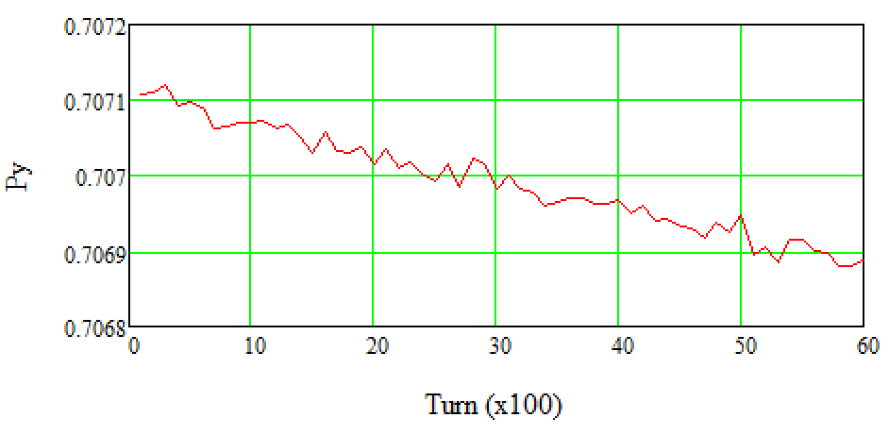
\includegraphics[width=0.9\linewidth]{2_polar1} \\ а)
    \end{minipage}
    \hfill
    \begin{minipage}[b][][b]{0.49\linewidth}\centering
        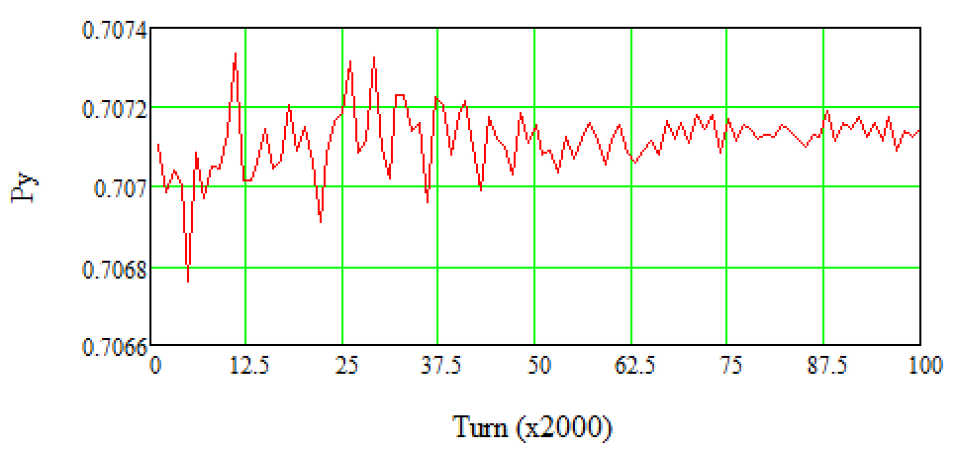
\includegraphics[width=0.9\linewidth]{2_polar2} \\ б)
    \end{minipage}
    \caption{Изменение поляризации во время процедуры скачка критической энергии: (а) ускорение на этапе 2, (б) скачок на этапе 3.}
    \label{fig:polar}
\end{figure}

\par При моделировании рассматриваются частицы с различными доступными начальными параметрами. Инжир. на рисунке \ref{fig:polar} показано изменение поляризации на 2-м (2 раза по $10^5$ оборотов) и 3-м (6 раз по $10^3$ оборота) этапах процедуры перехода. Поляризация здесь определяется как сумма проекций вектора спина на ось Y всех частиц и существенно не менялась в ходе процедуры. Стоит отметить, что COSY Infinity позволяет отслеживать вектор спина только для небольшого числа частиц, а не для ансамбля, что плохо для изучения поляризации.

\par Более подробно спиновая динамика будет рассмотрена в ЭДМ-эксперименте всего комплекса NICA-Nuclotron в Главе \ref{ch:EDM}.

\section*{Выводы}
\par Рассмотрена продольная динамика пучка вблизи критической энергии, а также при её пересечении. Такая особенность характерна для структуры, в которой энергия инжекции пучка меньше критической энергии установки и возникает необходимость её преодоления для ускорения до конечной энергии эксперимента.

\begin{enumerate}

\item Воздействие критической энергии на продольную динамику пучка вызывает увеличение фазового объёма в результате неадиабатичности и нелинейности движения в области энергии, близкой к критической;

\item Для преодоления критической энергии может быть применена процедура скачка, которая подразумевает кратковременное изменение дисперсионной функции. Это может быть достигнуто путём использования дополнительных квадруполей или квадруполей поворотной арки. В первом случае можно добиться сохранения частоты, а во втором — необходимо контролировать изменение рабочей точки и стабильность в поперечной плоскости. Таким образом, определяется величина и темп изменения критической энергии при проведении процедуры скачка;

\item Гармонический или барьерный тип ВЧ оказывает влияние на темп ускорения, а также продольное распределение внутри сепаратрисы. В сочетании со схемой процедуры скачка, необходимо сравнивать темп изменения критической энергии таким образом, чтобы относительный темп при пересечении критической энергии был в разы выше темпа ускорения;

\item Проведено исследование влияния простейших моделей импедансов на динамику. Результаты показали, что для интенсивных сгустков влияние импедансов оказывается значительным. Применение более точных моделей импедансов может существенно углубить понимание реальной динамики системы;

\item В условиях, близких к критическим для интенсивного пучка, развивается продольная микроволновая неустойчивость, которая существенно ограничивает характеристики пучка в конечном эксперименте и, в результате приводит к уменьшению светимости в коллайдере.

\end{enumerate}


\FloatBarrier
           % Глава 2
%part 3

	\chapter{Регулирование критической энергии методом резонансной вариации дисперсионной функции}\label{ch:resonant}

\par Эта глава посвящена особенностям резонансной структуры с возможностью вариации критической энергии. Рассматриваются также адаптации структуры коллайдера NICA с повышенным значением критической энергии, превышающим конечную энергию эксперимента, что обеспечивает возможность проведения столкновений лёгких поляризованных пучков протонов и дейтронов в SPD детекторе.

\par	Альтернативным способом, который применяется для того чтобы избегать потери стабильности, является создание или модификация структуры с заведомо большим значением критической энергии. Такая структура носит название резонансной \cite{senichev:resonant}, \cite{senichev:construction} и впервые была предложена при проектировании каонной фабрики \cite{kaon_tr} и других установках мирового уровня, например, Neutrino Factory в CERN \cite{neutrino_tr}, было реализовано в J-PARC для главного кольца \cite{JHP_tr}, \cite{J-PARK_tr}. Принципиальным отличием резонансной структуры от регулярной является обеспечение резонансного условия для количества суперпериодов и частоты бетатронных колебаний в горизонтальной плоскости. Однако, это справедливо только для не полностью регулярных структур, а содержащих модуляцию градиента квадруполей или кривизны орбиты. В таком случае, происходит изменение оптических функций ускорителя и варьирование критической энергии выше энергии эксперимента, в том числе до комплексных значений, полностью убирая зависимость установки от дополнительных процедур пересечения критической энергии. Такой подход позволяет получить нулевую дисперсию на прямых участках в силу подавления дисперсии на поворотных арках, путём выбора целого числа бетатронных колебаний и создания ахромата первого порядка. Кроме того, в подобной структуре может быть легко реализован и ахромат второго порядка путём расстановки секступолей через один суперпериод. Подобный подход способствует достижению достаточного значения динамической апертуры.

\par Как было показано в Главе \ref{ch:dual}, структура коллайдера NICA проектировалась как дуальная для работы в двух модах: для экспериментов с тяжелыми ионами $^{\mathbf{79}}{\mathbf{Au}}_{\mathbf{197}}$ и для экспериментов с поляризованными протонами и дейтронами $\mathbf{p, d}$. В этом случае проблем с прохождением критической энергии не возникает, что было изначально учтено при проектировании. Однако, спроектированная и построенная регулярная структура, выбранная для тяжелоионной программы, имеет фиксированное значение критической энергии и является характеристикой конкретной установки, то есть не отличается для разного сорта частиц. Характер поведения тяжелых ионов и легких частиц, существенно отличается с точки зрения внутрипучкового рассеяния. Для протонного пучка с интенсивностью $1\times10^{12}$ время внутрипучкового нагрева возрастает примерно в 10 раз по сравнению с пучками ионов золота с интенсивностью $2.2\times10^{9}$. Поэтому критическая энергия может подниматься за счет вариации дисперсии без опасения влияния внутрипучкового рассеяния. За счет резонансной модуляции дисперсионной функции коэффициент диффузии для внутрипучкового рассеяния возрастает в 2-3 раза, что не критично как при охлаждении протонов во время накопления, так и при их группировке на энергии эксперимента.

\par Как было показано в Главе \ref{ch:transition}, при прохождении через критическую энергию $\gamma_{\text{tr}}$ развивается продольная неустойчивость для интенсивных сгустков. Пороговый ток ее развития $I_{\text{th}}\sim\eta$ пропорционален коэффициенту расширения орбиты, который стремится к нулю в первом приближении при $\gamma=\gamma_{\text{tr}}=7.1$. Темп ускорения протонов при прохождении через критическую энергию при использовании индукционного ускорения в станции ВЧ1 составляет $\dv{\gamma}{t}=0.2~\text{c}^{-1}$. Этот темп слишком мал, чтобы полностью избежать развития неустойчивости при приближении релятивистского фактора к $\gamma_{\text{tr}}$. Чтобы исключить при ускорении протонов прохождение через критическую энергию, для протонной моды должна быть реализована новая оптическая структура колец вместо оптической структуры тяжелоионной моды. В этой оптической структуре критическая энергия должна быть выше максимальной энергии протонов при работе коллайдера на эксперимент.

\par Максимальная магнитная жесткость поворотных магнитов постоянна $R_{\text{arc}}\cdot B_{\text{bend}}=\frac{A\cdot m c\gamma\beta}{eZ}\approx45~\text{Тл}\cdot\text{м}$. В силу того, что отношения массы к заряду $\left(A/Z\right)_{\text{p}}=1/1=1$, для ионов золота $\left(A/Z\right)_{\text{Au}}=197/79=2.2$. Тем самым, определяется максимально возможная энергия для протонов $E_{\text{max}}^{\text{p}}~=~12.4$~ГэВ ($\gamma_{\text{p}}=14.3$), следовательно критическая энергия должна быть не менее ($\gamma_{\text{tr}}~=~15-16$), что заведомо выше критической энергии для ионной регулярной структуры $E_{\text{tr}}^{\text{Au}}=5.7$\ ГэВ ($\gamma_{\text{tr}}^{\text{Au}}=7,1$).

\par В данной главе будут приведено краткое теоретическое обоснование применения метода создания резонансной структуры. Теоретический метод был развит в работе \cite{senichev:resonant}, а его применение для современных ускорительных установок рассмотрено в работе \cite{senichev:construction}. Изучена возможность адаптации регулярной магнитооптической структуры главного кольца NICA к резонансной. А также анализ полученной структуры с точки зрения компенсации нелинейных эффектов, компенсации хроматичности и динамической апертуры.
  
\section{Введение суперпериодической модуляции}\label{sec:transition_variation/methods/resonant}

\par Здесь будет приведено кратное теоретическое обоснование метода резонансных структур, применяемых для обеспечения вариации критической энергии. Исходя из уравнения \ref{eq:alpha} коэффициент расширения орбиты $\alpha$ зависит как от дисперсионной функции $D(s)$, так и радиуса кривизны орбиты $\rho(s)$, таким образом вариация критической энергии может быть достигнута путем введения независимой модуляции обеих функций.

\par Уравнение для дисперсионной функции с бипериодической переменной фокусировкой \cite{senichev:resonant}:

\begin{equation}
\dv[2]{D}{s}+\left[K(s)+\varepsilon k(s)\right]D=\frac{1}{\rho(s)} ,
\label{eq:disp_eq}
\end{equation}

\noindent где $K\left(s\right)=\frac{e}{p}G\left(s\right), \varepsilon k\left(s\right)=\frac{e}{p}\Delta G\left(s\right), G\left(s\right)$ – градиент магнитооптических линз, $\Delta G\left(s\right)$ – суперпериодическая модуляция градиента, $p=\beta\gamma m_0 c$ – импульс частицы. Суперпериод определяется как совокупность нескольких периодов. Функция $K\left(s\right)$ имеет периодичность одного периода фокусирующей ячейки $L_{c}$, $k(s)$ и $\rho(s)$ имеют периодичность суперпериода $L_{\text{s}} = n \cdot L_{\text{c}}$.

\noindent Разложение в ряд  Фурье для зеркального суперпериода может быть осуществлено только по косинусам

\begin{equation}
\varepsilon k\left(\phi\right)=\sum_{k=0}^{\infty}g_{k}\cos(k\phi),
\label{eq:superperiodicity_fourier}
\end{equation}

\noindent где $\phi=\frac{2\pi}{L_s}s$ -- угловая продольная координата, $k$-ая гармоника:
\begin{equation}
g_k=\frac{1}{B\bar{R}} \frac{1}{\pi} \int_{-\pi}^\pi \Delta G \cos k \phi d \phi,
\end{equation}
\noindent где $B\bar{R}$ -- магнитная жесткость.

\noindent Радиус кривизны орбиты также может быть разложен в ряд Фурье по косинусам

\begin{equation}
\frac{1}{\rho(\phi)}=\frac{1}{\bar{R}}\left(1+\sum_{n=1}^{\infty} r_n \cos n \phi\right),
\end{equation}

\noindent где $n$-ая гармоника

\begin{equation}
r_n=\frac{\bar{R}}{\pi} \int_\pi^{-\pi} \frac{\cos n \phi}{\rho(\phi)} d \phi.
\end{equation}

\noindent Полученные разложения могут быть подставлены в уравнение \ref{eq:disp_eq}, из которого получено необходимое точное решение для дисперсионной функции $D(s)$. Таким образом, окончательно для коэффициента уплотнения орбиты одного суперпериода получено выражение в общем виде, разложенное до второго порядка

\begin{equation}
\begin{gathered}
\alpha_{\text{s}}=\frac{1}{\nu^2}\left\{1+\frac{1}{4}\left(\frac{\bar{R}}{\nu}\right)^4 \sum_{k=-\infty}^{\infty}\right.
\frac{g_k^2}{(1-k S / \nu)\left[1-(1-k S / \nu)^2\right]^2}+ \\
+\frac{1}{4} \sum_{k=-\infty}^{\infty} \frac{r_k^2}{1-k S / \nu} -\frac{1}{2}\left(\frac{\bar{R}}{\nu}\right)^2 \sum_{k=-\infty}^{\infty} \frac{r_k g_k}{(1-k S / \nu)\left[1-(1-k S / \nu)^2\right]} - \\
-\frac{1}{2}\left(\frac{\bar{R}}{\nu}\right)^2 \sum_{k=-\infty}^{\infty} \frac{r_k g_k}{1-(1-k S / \nu)^2}
\left.+O\left(g_k^i, r_k^j, i+j \geq 3\right)\right\},
\end{gathered}
\label{eq:alpha_general}
\end{equation}

\noindent где ${\overline{R}}_{\text{arc}}$ -- усредненное значение кривизны, $\nu=\nu_{x}$ -- количество горизонтальных бетатронных колебаний на длине арки, $S$ -- количество суперпериодов на длине арки. В случае отсутствия суперпериодической модуляции и модуляции кривизны орбиты $g_k=0, r_n=0 \  \forall~k, n$, формула \ref{eq:alpha_general} принимает вид $\alpha_{\text{s}}=\frac{1}{{\gamma_{\text{tr}}}^2}=\frac{1}{{\nu_x}^2}$, что соответствует случаю регулярной структуры, откуда видно, что $\gamma_{\text{tr}}\sim\nu_x$. Для поднятия критической энергии необходимо уменьшить коэффициент $\alpha_{\text{s}}=\frac{1}{{\gamma_{\text{tr}}}^2}$, а значит выражение под знаком суммы в ур. \ref{eq:alpha_general} должно быть отрицательным. Это реализуемо при условии $kS/\nu_{x}>1$, когда осуществлена либо модуляция градиентов квадруполей $g_k\not=0$, либо радиуса $r_n\not=0$.

\par Ранее все формулы были приведены для суперпериода, а не для всего кольца коллайдера. Введение прямых участков уменьшает степень модуляции дисперсионной функции. Усреднение дисперсии по более длинной орбите автоматически уменьшает ее значение, а значит уменьшает коэффициент уплотнения орбиты для всего ускорителя, результирующее значение критической энергии $\gamma_{\text{tr}}^{\text{total}}$ увеличивается и определяется выражением:

\begin{equation}
\gamma_{\text{tr}}^{\text{total}}=\gamma_{\text{tr}}^{\text{arc}}\sqrt{\frac{S\cdot L_{\text{s}}+L_{\text{str}}}{S\cdot L_s}},
\label {eq:gamma_tr_modulated}
\end{equation}

\noindent где $L_{\text{s}}$ -- длина суперпериода, $L_{\text{str}}$ -- длина бесдисперсионных прямых секций.

	\section{Построение резонансной структуры на основе ячеек ФОДО, ФДО, ОДФДО}\label{sec:transition_variation/methods/FODO_FDO}

Исходя из уравнения \ref{eq:alpha_general}, в случае отсутствия модуляции кривизны орбиты $r_n=0, \ \forall n$ для одного суперпериода в первом приближении (при $k=1$) коэффициент расширения орбиты приобретает вид
	
\begin{equation}
\begin{aligned}
\alpha_s= & \frac{1}{\nu^2}\left\{1+\frac{1}{4(1-k S / \nu)}\left(\frac{\bar{R}}{\nu}\right)^4 \frac{g_k^2}{\left[1-(1-k S / \nu)^2\right]^2}\right\}.
\end{aligned}
\label{eq:alpha_gradient}
\end{equation}

\noindent Таким образом, доступным средством вариации критической энергии, является только модуляция градиента квадрупольных линз по длине суперпериода. Одинаковые элементы, расположенные в различных местах арки, объединяют в одно семейство. На рис. \ref{fig:superperiod_3FODO} изображен один суперпериод, который состоит из 3-х ФОДО ячеек, c двумя семействами фокусирующих квадруполей (QF1 и QF2) и одним семейством дефокусирующих (QD).

\begin{figure} [h!]
   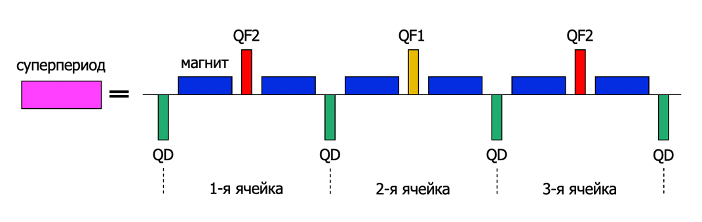
\includegraphics[width=1\columnwidth]{2_superperiod.png}
   \caption{Суперпериод, состоящий из 3-х ФОДО ячеек. QF1, QF2 -- фокусирующие квадруполи, QD -- дефокусирующие квадруполи.}
   \label{fig:superperiod_3FODO}
\end{figure}
	
\par Суперпериод может быть образован на основе синглетных ФОДО, дублетных ФДО, а также триплетных ОДФДО ячеек (рис.\ref{fig:fodo_fdo_odfdo} a,б,в). Рассмотрим структуры поворотных арок на 180 градусов без модуляции кривизны (рис.\ref{fig:fodo_fdo_odfdo} г, д, е), образованных из соответствующих ячеек. Из полученных суперпериодов также образуется резонансная магнитооптическая структура путем только модуляции градиента (рис.\ref{fig:fodo_fdo_odfdo} ж, з, и). Резонансная структура образуется путем вариации параметров регулярной структуры.

\begin{figure} [h!]

   \includegraphics*[width=.32\columnwidth]{2_twiss_fodo_cell.pdf}
   \includegraphics*[width=.32\columnwidth]{2_twiss_fdo_cell.pdf}
   \includegraphics*[width=.32\columnwidth]{2_twiss_odfdo_cell.pdf}

   \includegraphics*[width=.32\columnwidth]{2_twiss_fodo_resonant.pdf}
   \includegraphics*[width=.32\columnwidth]{2_twiss_fdo_resonant.pdf}
   \includegraphics*[width=.32\columnwidth]{2_twiss_odfdo_resonant.pdf}

   \caption{Твисс-параметры $\beta_{x,y}$, $D_{x}$. Сверху -- для ячеек для сигнлетной ФОДО, дублетной ФДО, триплетной ОДФДО ячеек; посредине -- регулярная структура; снизу -- резонансная.}
   \label{fig:fodo_fdo_odfdo}
\end{figure}

\par Качественное отличие в пространственном распределении Твисс-параметров $\beta_{x}$, $\beta_{y}, D_{x}$ является ключевым для соответствующей оптимизации структуры.
Как видно из приведенных структур, суперпериод, основанный на синглетных ФОДО ячейках, может иметь ряд преимуществ.

\noindent Хроматичность зависит от величины градиентов в квадруполях, секступолях, а также местах их расположения \cite{lee}

\begin{equation}
\begin{aligned}
& C_x=-\frac{1}{4 \pi} \oint \beta_x\left[K_x(s)-S(s) D(s)\right] \textrm{d} s, \\
& C_y=-\frac{1}{4 \pi} \oint \beta_y\left[K_y(s)+S(s) D(s)\right] \textrm{d} s.
\end{aligned}
\end{equation}

\noindent Отсюда видно, что, во-первых, для подавления хроматических эффектов в ФОДО-ячейке, требуются меньшие градиенты в секступольных линзах. Во-вторых, более простой способ коррекции и тонкой настройки набега бетатронных частот в обеих плоскостях, а также коэффициента расширения орбиты. Таким образом, является более предпочтительной по сравнению с аналогичными.

	\section{Регулярная ФОДО структура с суперпериодической модуляцией градиентов линз}\label{sec:transition_variation/methods/FODO}

\par Поскольку квадрупольная фокусирующая структура поворотных арок коллайдера NICA состоит из ФОДО ячеек, рассмотрим возможность адаптации регулярной структуры к резонансной. На рис. \ref{fig:twiss_3FODO} приведены 3 ФОДО ячейки, первая – используется в регулярной тяжелоионной структуре, в этом случае модуляция отсутствует, вторая – модулированная структура,  которая и образует один суперпериод. В обоих случаях частота бетатронных колебаний для одного суперпериода $\nu_{x,y}=0.75$, таким образом для 4-х суперпериодов частота $\nu_{x,y\ \text{arc}}=3$, что удовлетворяет ранее рассмотренному условию $S=4, \nu_x=3$.

\begin{figure}[h!]
	\includegraphics*[width=.49\columnwidth]{2_twiss_3FODO_regular}
	\includegraphics*[width=.49\columnwidth]{2_twiss_3FODO_modulated}
	\caption{Твисс-параметры 3-х ячеек. Слева – регулярная структура без модуляции, справа – модулированная c введением суперпериодичности, глубина модуляции 24\%.}
	\label{fig:twiss_3FODO}
\end{figure}

\noindent Глубина модуляции определяется соотношением градиентов двух различных фокусирующих семейств. Для приведенного на правом рисунке рис. \ref{fig:twiss_3FODO} $G_{\textrm{QF1}}~=~27.7$~Тл/м, $G_{\textrm{QF2}}~=~21.0$~Тл/м. Таким образом глубина модуляции:

\begin{equation}
H=\frac{G_{\textrm{QF1}}-G_{\textrm{QF2}}}{G_{\textrm{QF1}}}=24\%
\label {eq:modulated_coeff}
\end{equation}

\noindent Первая гармоника является определяющей, и для 12 ФОДО ячеек реализуемо условие $S=4, \nu_x=3$, где 3 ФОДО ячейки объединены в один суперпериод. Таким образом, благодаря набегу бетатронных колебаний кратному $2\pi$, в нашем случае $6\pi$, арка имеет свойства ахромата первого порядка. Благодаря этому свойству может быть подавлена дисперсия без дополнительных усилий.

\noindent Для арки, составленной из 4-х одинаковых суперпериодов с критической энергией на арке $\gamma_{\text{tr}}^{\text{arc}}=\ 10$, по формуле \ref{eq:gamma_tr_modulated} для всего кольца получаем $\gamma_{\text{tot}}^{\text{arc}}\ \approx\ 15.9$. Однако, конечная арка будет нерегулярной в силу необходимости подавления дисперсии на краях арки, а значит в конкретном реальном случае значение критической энергии будет несколько отличаться.

\section{Подавление дисперсии}\label{sec:transition_variation/disp_supperssion}

\par Обеспечение нулевого значения дисперсии на прямых участках необходимо для обеспечения движения частиц вдоль несмещённой равновесной орбиты. Это условие легко реализуется при подавлении дисперсии и её производной на концах поворотной арки. Рассматривается 4 варианта подавления дисперсии:

\begin{enumerate} 
\item	Полностью регулярная арка. \ Регулярная арка состоящая из 4-х одинаковых суперпериодов. При набеге фазы на арке кратному $2\pi$ подавление дисперсии происходит в силу регулярности;
\item Регулярная арка с применением методики отсутствующих магнитов на двух крайних ячейках арки, что показано на рис. \ref{fig:2_disp_supp}.
\item В структуре с отсутствующими магнитами при переходе к резонансной оптике, подавление дисперсии возможно при помощи крайних суперпериодов. В этому случае при набеге фазы на арке не кратному $2\pi$ необходимо дополнительно добавить подавители дисперсии на краях арки, а именно двух крайних ФОДО ячеек. Две крайние ФОДО ячейки отличаются наличием и в этих ячейках квадруполи QFE1 и QFE2 также имеют отличные градиенты от основных квадруполей арки и подбираются таким образом, чтобы подавить дисперсию.
\item В структуре с отсутствующими магнитами при переходе к резонансной оптике, также возможно подавление дисперсии всей аркой, при помощи выбора градиентов квадруполей двух семейств. Этот случай отличается тем, что все квадруполи арки принадлежат первому, либо второму семейству и подавление дисперсии также обеспечивается только 2-мя семействами.
\end{enumerate} 

\noindent Дефокусирующие же квадруполи во всех случаях принадлежат только одному семейству QD. Рассмотрим представленные случаи  более подробно.

\begin{figure} [h!]
	\center
	\includegraphics*[width=.6\columnwidth]{2_disp_supp}
	\caption{Подавление дисперсии в тяжелоионной структуре.}
	\label{fig:2_disp_supp}
\end{figure}

\subsection{Полностью регулярная магнитооптическая структура}\label{subsec:transition_variation/disp_supperssion/regular}

\par Требование подавления дисперсии легко реализуемо в случае создания регулярных поворотных арок, составленных из одинаковых суперпериодов. В этом случае, обеспечив нулевое значение дисперсии $D=0$ (а также производной дисперсии $D^{\prime}=0$) на входе в арку, в силу регулярности на выходе из арке также будут нулевые значения дисперсии и её производной, а следовательно и на всем прямом участке. Однако, учитывая особенность структуры коллайдера NICA, наличие отсутствующих магнитов на двух крайних ячейках не дает возможность создать полностью регулярную арку из 4-х одинаковых суперпериодов.

\begin{figure} [h!]
   \center
   \includegraphics*[width=1.\columnwidth]{2_supp_scheme_regular.png}
   \includegraphics*[width=1.\columnwidth]{2_supp_Twiss_regular.png}
   \includegraphics*[width=1.\columnwidth]{2_supp_elem_regular.png}
   \caption{Подавление дисперсии в регулярной структуре.}
   \label{fig:2_disp_supp_full_regular}
\end{figure}
	
\subsection{Подавление дисперсии при помощи крайних суперпериодов}\label{subsec:transition_variation/disp_supperssion/ES}

\par	
\begin{figure} [h!]
   \center
   \includegraphics*[width=1.\columnwidth]{2_supp_scheme_ES.png}
   \includegraphics*[width=1.\columnwidth]{2_supp_Twiss_ES.png}
   \includegraphics*[width=1.\columnwidth]{2_supp_elem_ES.png}
   \caption{Подавление дисперсии в тяжелоионной структуре.}
   \label{fig:2_disp_supp_ES}
\end{figure}		

\par В этому случае выбор значения градиентов квадруполей арки определяется двумя факторами:
	а) получение необходимого значения критической энергии на всем кольце коллайдера, что соответствует $\gamma_{\text{tr}}\sim15-16$;
	б) обеспечение количества бетатронных колебаний на арке $\nu_{\text{arc}}=3$ в обеих плоскостях, тем самым удовлетворив резонансному условию при количестве суперпериодов $S=4$. Исходя из этих условий модулируем суперпериод с набегом фазы на суперпериоде $\nu_{\text{s}}=0.75$ в обоих плоскостях.

\par Коллайдер также состоит из 2-х арок и 2-х прямых участков, соединяющих арки. В центре прямых участков имеются точки столкновения, где нужно обеспечить малое значение бета-функции для достижения требуемой светимости. В крайнем суперпериоде применяется метод отсутствующих магнитов в 2-х ячейках, тем самым делая арки коллайдера не регулярными и возникает необходимость подавления дисперсии на прямых участках при помощи введения 2-х дополнительных семейств квадруполей QFE1 и QFE2 на краю арки, параметры Твисса изображены на рис. \ref{fig:2_disp_supp_ES}. В результате значение критической энергии подобрано таким образом, что $\gamma_{\text{tr}}=15.6$, а количество колебаний на арке: $\nu_{x,\ \text{arc}}=3.01,\ \nu_{y,\ \text{arc}}=3.01$.

\subsection{Подавление дисперсии всей аркой, при помощи выбора градиентов квадруполей двух семейств.}\label{subsec:transition_variation/methods/disp_supperssion_AS}	

Данный способ показывает возможность подавления дисперсии на прямых участках при помощи только двух семейств фокусирующих квадруполей. Тут, как и в первом случае, необходимо выполнить:
	а) получение значения критической энергии на всем кольце коллайдера, что соответствует $\gamma_{\text{tr}}\sim15-16$;
	б) только при помощи квадруполей двух семейств подавить дисперсию на прямых участках.

\begin{figure} [h!]
	\center
	\includegraphics*[width=1.\columnwidth]{2_supp_scheme_AS.png}
	\includegraphics*[width=1.\columnwidth]{2_supp_Twiss_AS.png}
	\includegraphics*[width=1.\columnwidth]{2_supp_elem_AS.png}
	\caption{Подавление дисперсии в тяжелоионной структуре.}
	\label{fig:2_disp_supp_AS}
\end{figure}
	
\par Изначально выбирается суперпериод, как и в первом случае, с набегом на суперпериоде $\nu_s=0.75$. Тем самым получаем значения квадруполей QF1 и QF2 для всей арки, в том числе и на краях. Однако, получается, что дисперсия на прямых участках оказывается не подавлена. Для подавления значения градиентов квадруполей изменяется, но в таком случае набег фазы на арке становится равен $\nu_{x,\ \text{arc}}=2.72178$,\ $\nu_{y,\ \text{arc}}=2.99884$, то есть в $x$–плоскости не кратен $2\pi$. В этом случае для достижения требуемого значения критической энергии необходимо обеспечить бОльшую модуляцию градиентов квадруполей, чем в случае подавления дисперсии крайними суперпериодами. Принципиальная схема показана на рис. \ref{fig:DA_AS_dpp}. Для полученной нерегулярной арки значение критической энергии $\gamma_{\text{tr}}^{\text{arc}}=\ 10$.

\section{Исследование динамической апертуры в синхротроне с учётом требуемой модуляции дисперсионной функции для повышения критической энергии}

\begin{figure} [h!]
	\center
	\includegraphics*[width=0.49\columnwidth]{2_ES_x_dpp0.png}
	\includegraphics*[width=0.49\columnwidth]{2_ES_y_dpp0.png}
	\includegraphics*[width=0.49\columnwidth]{2_ES_x_dpp0,3.png}
	\includegraphics*[width=0.49\columnwidth]{2_ES_y_dpp0,3.png}
	\includegraphics*[width=0.49\columnwidth]{2_ES_x_dpp0,5.png}
	\includegraphics*[width=0.49\columnwidth]{2_ES_y_dpp0,5.png}
	\caption{Динамическая аппретура для случая плавления дисперсии крайними квадруполями. 
		Слева – $x$-плоскость; справа – $y$-плоскость.}
	\label{fig:DA_ES_dpp}
\end{figure}	

\begin{figure} [h!]
   \center
   \includegraphics*[width=0.49\columnwidth]{2_AS_x_dpp0.png}
   \includegraphics*[width=0.49\columnwidth]{2_AS_y_dpp0.png}
   \includegraphics*[width=0.49\columnwidth]{2_AS_x_dpp0,3.png}
   \includegraphics*[width=0.49\columnwidth]{2_AS_y_dpp0,3.png}
   \includegraphics*[width=0.49\columnwidth]{2_AS_x_dpp0,5.png}
   \includegraphics*[width=0.49\columnwidth]{2_AS_y_dpp0,5.png}
   \caption{Динамическая апертура в случае подавление дисперсии двумя семействами квадруполей.
Слева – $x$-плоскость; справа – $y$-плоскость.}
   \label{fig:DA_AS_dpp}
\end{figure}

\par Выбор нечётного значения частоты на арке $\nu_{x,\ \text{arc}}=3$ и чётного значения суперпериодичности арки $S=4$ замечателен еще и тем, что позволяет компенсировать нелинейный вклад секступолей внутри арки. Добавление секступолей, подавляющих хроматичность внутри арки делает арку ахроматом второго порядка, что убирает зависимость бетатронных колебаний от импульса и способствует сохранению динамической апертуры в большом диапазоне энергий. В этом случае набег фазы радиальных колебаний между ячейками, расположенными в разных половинках арки и разделенных $S/2$ числом суперпериодов равен:

\begin{equation}
2\pi\cdot\frac{\nu_{\text{arc}}}{S_{\text{arc}}}\cdot\frac{S_{\text{arc}}}{2}=2\pi\cdot\frac{\nu_{\text{arc}}}{2}=\pi+2\pi n,\
\label{eq:chrom_period}
\end{equation}

\noindent что соответствует условию компенсации нелинейного влияния секступолей в первом приближении во всей арке. Это замечательное свойство также относится к высшим мультиполям в квадруполях и отклоняющих магнитах. Эта связь через число суперпериодов $S_{\text{arc}}/2$ называется длинной связью.

\section*{Выводы}
\par Рассмотрена методика вариации критической энергии методом модуляции градиента квадрупольных линз на арках. Такой случай предполагает раздельное питание квадруполей. Также учтена необходимость подавления дисперсии на краях арки в имеющейся структуре и подавление хроматичности на всем кольце коллайдера. Исследования выполнены в применении к ускорительному комплексу NICA, однако без потери общности, может применяться на различных установках.

\begin{enumerate}

\item Введение модуляции дисперсионной функции или радиуса кривизны орбиты приводит к вариации коэффициента уплотнения орбиты и как следствие критической энергии установки. Таким образом можно добиться повышенной критической энергии, выше энергии эксперимента, и также достижения комплексного значения;

\item Рассмотрены схемы подавления дисперсионной функции в резонансной структуре на краях поворотных арок. В случае полностью регулярной структуре это достигается путем выбора кратного набега фазы. При использовании метода отсутствующих магнитов ('missing magnet'), регулярность нарушается и возможно подавление как крайними ячейкам, так и только двумя семействами квадруполей;

\item Исследовано влияние нелинейных эффектов на динамическую апертуру в резонансной структуре. Для различных вариаций магнитооптики предложены оптимальные схемы расстановки секступолей.

\end{enumerate}

\FloatBarrier           % Глава 3
%part 4
%	\chapter{Изучение особенностей магнитооптической структуры синхротронов NICA и Nuclotron с учетом %ускорения поляризованных пучков и модернизация магнитооптической структуры Nuclotron с учётом возможности %изучения ЭДМ}\label{ch:EDM}

	\chapter{Изучение особенностей магнитооптической структуры синхротронов для ускорения поляризованных пучков с учётом возможности изучения ЭДМ}\label{ch:EDM}

\par Электрический дипольный момент (ЭДМ) элементарных частиц обусловлен неоднородностью распределения заряда. Необходимость такой неоднородности была установлена Сахаровым для объяснения механизма CP-нарушения \cite{sakharov}. Наличие ненулевого МДМ и ЭДМ может оказывать воздействие на поведение спина в электромагнитном поле.  Стоит отметить, что спин отдельной частицы является квантовой величиной, однако его поведение в ансамбле описывается классически, что было показано Tompson и Telegdi, Bargmann, Michel \cite{TBMT}. Поведение спина ансамбля частиц описывается одноименным классическим уравнением T-БМТ, где спин является описывается вектором

\begin{align} \label{eq:T-BMT}
\frac{{d \vec{S}}}{d t} &=\vec{S} \times\left(\vec{\Omega}_{\textrm{MDM}}+\vec{\Omega}_{\textrm{EDM}}\right), \nonumber\\
\vec{\Omega}_{\textrm{MDM}}&=\frac{q}{m \gamma}\left\{(\gamma G+1)\vec{B}_{\perp}+(G+1)\vec{B}_{\parallel}-\left(\gamma G+\frac{\gamma}{\gamma+1}\right) \frac{\vec{\beta} \times \vec{E}}{c}\right\}, \\
\vec{\Omega}_{\textrm{EDM}}&=\frac{q \eta}{2 m}\left(\vec{\beta} \times \vec{B}+\frac{\vec{E}}{c}\right), \quad G=\frac{g-2}{2},\nonumber
\end{align}

\noindent где $\vec{\Omega}_{\textrm{MDM}}, \vec{\Omega}_{\textrm{EDM}}$ -- угловые частоты обусловленные наличием магнитного дипольного момента (МДМ) и электрического дипольного момента (ЭДМ); $q, m, G$ -- заряд, масса и магнитная аномалия; $\beta$ -- нормализованная скорость; $\gamma$ -- Лоренц-фактор; $d =~\eta \frac{q}{2mc}s$ -- ЭДМ фактор, $s$ -- спин. Уравнение содержит 2 слагаемых, одно обусловлено наличием МДМ, другое – ЭДМ соответственно \cite{silenko:edm}. Для непосредственного измерения ЭДМ-компоненты, влияние МДМ на спин должно быть нивелировано.

\par Помимо, рассмотренного в Главах \ref{ch:dual}-\ref{ch:resonant}, коллайдера NICA, в ускорительный комплекс также входит установка Nuclotron \cite{nuclotron24}. Данный синхротрон предназначен как для самостоятельных экспериментов на выведенной мишени BM@N и изучения управления поляризацией, так и для использования в качестве инжектора поляризованного пучка протонов и дейтронов в коллайдер NICA. Однако, установка была введена в эксплуатацию в 90-е годы \cite{baldin:nuclotron} и может быть модернизирована с использованием новых современных магнитооптических элементов, производимых непосредственно в ОИЯИ г. Дубна \cite{korovkin:nica_magnets}. Для расширения возможностей Nuclotron в качестве самостоятельной машины рассматривается возможность изучения ЭДМ легких заряженных частиц. Такие прецизионные эксперименты возможны на ускорителе, работающем в режиме накопительного кольца с целью долгого удержания сгустка на орбите и накоплению достаточной статистики эксперимента. 

\par Возможность исследования ЭДМ с применением метода квази-замороженного спина возможна также и на установке, изначально для этого не предназначенной. Однако, поскольку для компенсации влияния МДМ необходимо использование элементов с электрическим полем, требуется дополнительное место для их расположение. Такое может быть достигнуто путем введения обводных каналов. Это возможно в том числе в кольце коллайдера NICA.

\par В экспериментах по измерению ЭДМ ключевым является обеспечение высокого показателя времени когерентности (SCT — Spin Coherence Time) порядка 1000 с \cite{AGSproposal}. В течение такого времени когерентный поляризованный пучок удерживается на орбите. Таким образом, для моделирования структуры с возможностью исследования ЭДМ необходимо гарантировать стабильность спиновой динамики вдоль всего кольца, что является отдельной задачей, наравне с обеспечением орбитальной стабильности пучка.

\section{Орбитальная и спиновая динамика в электромагнитных полях}\label{sec:EDM/requirements/deflector}

\par Рассмотрим как орбитальное, так и спиновое движение в электромагнитных полях. Для орбитального вращения в поперечном магнитном поле согласно уравнению Лоренца

\begin{equation} \label{eq:lorenz}
qc\vec{\beta}\times{\vec{B}}_\bot={\vec{\Omega}}_p^{\textrm{B}}\times\vec{p},
\end{equation}

\noindent где $q$ -- заряд, $c$ -- скорость света, $\vec{\beta}$ -- вектор относительной скорости, ${\vec{B}}_\bot$ -- поперечное магнитное поле, $\vec{p}$ -- импульс частицы, ${\vec{\Omega}}_p^{\textrm{B}}$ -- вектор угловой скорости (индексы означают, что происходит вращение импульса в магнитном поле). Учтем, что импульс частицы представим в виде $\vec{p}\ =\ \gamma mc\vec{\beta}$, тогда ур.\ref{eq:lorenz} с учетом перестановки векторного произведения получаем

\begin{equation}	
qc\vec{\beta}\times{\vec{B}}_\bot=-mc\gamma\vec{\beta}\times{\vec{\Omega}}_p^{\textrm{B}},
\end{equation}

\noindent для угловой скорости

\begin{equation} \label{eq:omega_pB}
 {\vec{\Omega}}_p^{\textrm{B}}=-\frac{q}{m\gamma}{\vec{B}}_\bot.
\end{equation} 

\begin{figure}[!h]
  \centering
	\includegraphics*[width=0.49\columnwidth]{4_orbital_B}
	\includegraphics*[width=0.49\columnwidth]{4_orbital_E}
   \caption{Вращение положительно заряженной частицы а) в магнитном поле; б) электростатическом поле.}
   \label{fig:4_orbital_B_E}
\end{figure}

\par Для заряженной частицы в электростатическом дефлекторе, выполняющего функцию поворота всегда соблюдается условие $\vec{p} \bot \vec{E}$, тогда происходит движение по окружности (рис.\ref{fig:4_orbital_B_E}) и аналогично ур.\ref{eq:lorenz}

\begin{equation}
q{\vec{E}}_\bot={\vec{\Omega}}_p^{\textrm{E}}\times\vec{p},
\end{equation} 

\noindent где ${\vec{E}}_\bot$ – электростатическое поле перпендикулярное импульсу, ${\vec{\Omega}}_p^{\textrm{E}}$ – вектор угловой скорости (индексы означают, что происходит вращение импульса в электростатическом поле)

\begin{equation}
q{\vec{E}}_\bot=mc\gamma{\vec{\Omega}}_p^{\textrm{E}}\times\vec{\beta}.
\end{equation} 

\noindent Для угловой скорости с учётом векторного произведения $\vec{v}=\vec{\omega}\times\vec{r}, \vec{\omega}=\frac{\vec{r}\times\vec{v}}{(\vec{r},\vec{r})}$

\begin{equation}
{\vec{\Omega}}_p^{\textrm{E}}=\frac{q}{mc}\frac{\vec{\beta}\times{\vec{E}}_\bot}{\gamma(\vec{\beta},\vec{\beta})}=\frac{q}{m\gamma}\frac{\vec{\beta}\times{\vec{E}}_\bot}{c\beta^2}\ \ \ 
\end{equation}

\par Рассмотрим теперь вращение спинового вектора под действием МДМ относительно вектора импульса

\begin{equation}
{\vec{\omega}}_p^{\textrm{B}}={\vec{\Omega}}_{\textrm{MDM}}^\textrm{B}-{\vec{\Omega}}_p^{\textrm{B}}=-\frac{q}{m\gamma}\left(\gamma G+1\right){\vec{B}}_\bot+\frac{q}{m\gamma}{\vec{B}}_\bot=-\frac{q}{m}{G\vec{B}}_\bot.
\end{equation}

\noindent Величина $\nu_s^{\textrm{B}}$ -- спин-тюн (spin-tune) является скалярной величиной и отражает во сколько раз поворот вектора спина больше поворота вектора импульса

\begin{equation} \label{eq:spintune_B}
\nu_s^{\textrm{B}}=\frac{\left|{\vec{\Omega}}_{\textrm{MDM}}^{\textrm{B}}-{\vec{\Omega}}_p^{\textrm{B}}\right|}{\left|{\vec{\Omega}}_p^{\textrm{B}}\right|}=\frac{-\frac{q}{m}{G\left|\vec{B}\right|}_\bot}{-\frac{q}{m\gamma}\left|{\vec{B}}_\bot\right|}=\gamma G.
\end{equation}

\noindent Аналогично для вращения в электростатическом поле
\begin{equation}
\begin{aligned}
{\vec{\omega}}_p^{\textrm{E}}={\vec{\Omega}}_{\textrm{MDM}}^{\textrm{E}}-{\vec{\Omega}}_p^{\textrm{E}}&=\frac{q}{m}\left(G+\frac{1}{\gamma+1}\right)\frac{\vec{\beta}\times\vec{E}}{c}-\frac{q}{mc}\frac{\vec{\beta}\times\vec{E}}{\gamma\beta^2} =\\
&=\frac{q}{mc}\left(G-\frac{1}{\gamma^2-1}\right)\vec{\beta}\times\vec{E}.
\end{aligned}
\end{equation}

\noindent Спин-тюн в электростатическом поле

\begin{equation} \label{eq:spintune_E}
\nu_s^{\textrm{E}}=\frac{\left|{\vec{\Omega}}_{\textrm{MDM}}^{\textrm{E}}-{\vec{\Omega}}_p^{\textrm{E}}\right|}{\left|{\vec{\Omega}}_p^{\textrm{E}}\right|}=\frac{\frac{q}{mc}\left(G-\frac{1}{\gamma^2-1}\right)\left|\vec{\beta}\times\vec{E}\right|}{\frac{q}{mc}\frac{\left|\vec{\beta}\times\vec{E}\right|}{\gamma\beta^2}}=\gamma\beta^2\left(G-\frac{1}{\gamma^2-1}\right).
\end{equation}
Примечательно, что спин-тюн как в магнитном поле ур.\ref{eq:spintune_B}, так и  электростатическом ур.\ref{eq:spintune_E} не зависит от величины поля в дефлекторе.

\section{Общий концепт квазизамороженной структуры}\label{sec:EDM/requirements/deflector}

\par Перейдем от рассмотрения общего случая вращения спина в магнитном и электрическом поле к непосредственным элементам и поворотным аркам. Из уравнений \ref{eq:spintune_B}, \ref{eq:spintune_E} видно, что для спиновой динамики сорт частиц существенно влияет на вращение относительно импульса. Для удобства повествования, все рассуждения и рисунки будут приведены для дейтрона, без потери общности, в дальнейшем будет рассмотрен и случай протонов.

\par Вращение в чисто магнитном кольце, содержащем в  поворотной арке только дипольные магниты, происходит под действием поперечного магнитного поля на $2\pi$, при этом поворот вектора импульса за один период осуществляется на $\Phi_p^{\textrm{arc}}=\sfrac{2\pi}{N}$, где $N$ – количество периодов, магнитных арок. Поворот спина, относительно спина происходит пропорционально $\gamma G$

\begin{equation}
\Phi_s^{\textrm{arc}}=\gamma G\cdot\Phi_p^{\textrm{arc}}.
\end{equation}

\begin{figure}[!h]
  \centering
	\includegraphics*[width=0.39\columnwidth]{4_arc_B}
	\includegraphics*[width=0.59\columnwidth]{4_arc_B+E}
   \caption{Отклонение спин-вектора в арке относительно импульса в случае дейтрона}
    \label{fig:4_arc_B_E}
\end{figure}

\noindent Принципиальная схема вращения импульса и спина пучка дейтронов показана для магнитной арке на рисунке \ref{fig:4_arc_B_E}a.

\par Рассмотрим простейший случай одного периода, состоящего из магнитной и электростатической арок, в котором может быть реализована компенсация МДМ-компоненты методом квази-замороженного спина. В отсутствии электростатических дефлекторов, вращение импульса в магнитной арке происходит на $\Phi_p^{\textrm{arc}}=\sfrac{2\pi}{N}$. При необходимости введения электростатической арки с отрицательной кривизной $\Phi_{p\textrm{E}}^{\textrm{def}}$, магнитные арки должны дополнительно поворачивать на угол $\Phi_{p\textrm{B}}^{\textrm{kick}}$ при помощи киккеров. Такой поворот будет впоследствие скомпенсирован поворотом в электростатической арке. На рис. \ref{fig:4_arc_B_E}б изображено поведения спин-вектора для дейтрона при последовательном действии магнитной арки, киккера, электростатической арки с отрицательной кривизной, киккера. Поворот импульса, после прохождения периода должен также быть повернуть на $\sfrac{2\pi}{N}$. Окончательно, 

\begin{equation}
\Phi_p^{\textrm{arc}}+\Phi_{p\textrm{B}}^{\textrm{kick}}+\Phi_{p\textrm{E}}^{\textrm{def}}=\frac{2\pi}{N}\ \ \
\end{equation}
или с учетом поворота в магнитной арке
\begin{equation}
\Phi_{p\textrm{B}}^{\textrm{kick}}={-\Phi}_{p\textrm{E}}^{\textrm{def}}\ \ \ 
\end{equation}


\noindent Спин-вектор в магнитной арке совершит отклонение в магнитном поле $\Phi_{s\textrm{B}}^{\textrm{arc+kick}}=\nu_s^{\textrm{B}}\left(\Phi_p^{\textrm{arc}}+\Phi_{p\textrm{B}}^{\textrm{kick}}\right)$. В электростатической арке $\Phi_{s\textrm{E}}^{\textrm{def}}=\nu_s^{\textrm{E}}\Phi_{p\textrm{E}}^{\textrm{def}}$. 
Отдельно для спинового движения, в киккерах и дефлекторе
\begin{equation}
\begin{aligned}
\Phi_s^{\textrm{kick+def}}  & = \nu_s^{\textrm{B}} \Phi_{p\textrm{B}}^{\textrm{kick}}+\nu_s^{\textrm{E}} \Phi_{p\textrm{E}}^{\text {\textrm{def}}}= \\
				& = \Phi_{p\textrm{B}}^{\textrm{kick}}\left[\gamma G-\beta^2 \gamma\left(G-\frac{1}{\gamma^2-1}\right)\right]= \\
				& = \Phi_{p\textrm{B}}^{\textrm{kick}}\left[\frac{G+1}{\gamma}\right]
\end{aligned}
\label{eq:spin_kick}
\end{equation}

\noindent Условие сохранения ориентации спин-вектора, то есть условие «квази-замороженности» можно записать в виде
\begin{equation}
\Phi_s^{\textrm{arc}}+\Phi_s^{\textrm{kick+def}}=0
\label{eq:QFS_condition}
\end{equation}

\noindent Тогда из уравнений \ref{eq:spin_kick} -- \ref{eq:QFS_condition} для 

\begin{equation} \label{eq:kick}
\Phi_{p\textrm{B}}^{\textrm{kick}}=-\Phi_p^{\textrm{arc}}\frac{\gamma^2G}{G+1}=-\frac{2\pi}{N}\frac{\gamma^2G}{G+1}\ \
\end{equation}

\noindent Отсюда видно, что кривизна дефлектора для дейтрона должна быть отрицательна, поскольку аномальный магнитный момент дейтрона отрицательный и меньше единицы $G_{\textrm{d}} = -0.142$.

\par Рассмотрим движение в прямом фильтре Вина. Ключевое условие -- равенство нулю силе Лоренца, таким образом фильтр Вина не отклоняет орбитальное движение
\begin{equation}
q\left(c\vec{\beta}\times{\vec{B}}_\bot+{\vec{E}}_\bot\right)=0.
\end{equation}
\noindent Стоит отметить, при этом выполняется равенство магнитного и электростатического абсолютных радиусов $\left|R_{\textrm{E}}\right|=\left|R_{\textrm{B}}\right|$ и для углов поворота
\begin{equation}
\Phi_{p\textrm{B}}^{\textrm{WF}}+\Phi_{p\textrm{E}}^{\textrm{WF}}=0\ \ \ 
\Phi_{p\textrm{B}}^{\textrm{WF}}=-\Phi_{p\textrm{E}}^{\textrm{WF}}=\Phi_p^{\textrm{WF}}.
\end{equation}

\noindent Поскольку импульс в фильтре Вина остается неизменным, то результирующее вращение спина может быть рассмотрено также относительно импульса. При этом необходимо подавить вращение от магнитной арки $\Phi_s^{\textrm{arc}}=\gamma G\cdot\Phi_p^{\textrm{arc}}$.
Таким образом условие «квази-замороженности» может быть записано аналогично ур. \ref{eq:QFS_condition} как 
\begin{equation}
\Phi_s^{\textrm{WF}}+\Phi_s^{\textrm{arc}}=0.
\end{equation}

\noindent Для спинового движения в фильтре Вина под действием МДМ выполняется

\begin{equation} \label{eq:spin_kick_WF}
\begin{aligned}
 \Phi_s^{\textrm{WF}} & =  \nu_s^{\textrm{B}} \Phi_{p\textrm{B}}^{\textrm{WF}}+\nu_s^{\textrm{E}} \Phi_{p\textrm{E}}^{\textrm{WF}}= \\
			& =  \Phi_p^{\textrm{WF}}\left[\gamma G-\beta^2 \gamma\left(G-\frac{1}{\gamma^2-1}\right)\right]= \\
			& =  \Phi_p^{\textrm{WF}}\left[\frac{G+1}{\gamma}\right]
\end{aligned}
\end{equation}

\noindent что совпадает с уравнением \ref{eq:spin_kick}. А значит и для угла поворота в фильтре Вина, аналогично ур. \ref{eq:kick}
\begin{equation}
\Phi_p^{\textrm{WF}}=-\Phi_p^{\textrm{arc}}\frac{\gamma^2G}{G+1}=-\frac{2\pi}{N}\frac{\gamma^2G}{G+1}.
\end{equation}

\par Такой результат говорит о том, что принципиальным для реализации квази-замороженности остается наличие отклоняющих полей. При использовании чисто электростатических дефлекторов, необходимо использовать дополнительный внешний магнитный толчок. В случае же прямого фильтра Вина используется скрещенные магнитное и электростатическое поля. Интегральная величина поля при этом сохраняется.

	\subsection{Длина компенсирующего элемента с электрической компонентой}\label{sec:EDM/requirements/length}
\par Радиус кривизны элемента с электрическим и магнитным полем может быть найден как
\begin{equation}
\begin{gathered}
\frac{1}{R}  = \frac{1}{R_\textrm{B}}+\frac{1}{R_\textrm{E}}, \ \ 
	R_\textrm{B}  = \frac{B\rho}{B}, \ \ 
	R_\textrm{E}  = \frac{\kappa}{E}, \ \ 
\end{gathered}
\end{equation}
где $B\rho=\sfrac{p_0}{e}$ – магнитная жесткость, $p_0=\gamma m\beta c$, $\kappa=\sfrac{p_0\beta c}{e}$ – электрическая жесткость.
Поскольку для фильтра Вина $R=\inf$, то и радиусы кривизны связаны $R_{\textrm{B}}=-R_{\textrm{E}}$. И для выбора радиуса достаточно определить либо магнитное поле, либо электрическое. Более строгое ограничение дается на электрическое поле $E_{\textrm{max}}=10\div13$ МВ/м.
Для нахождения длины
\begin{equation}
L={\Phi_p^{\textrm{WF}}R}_E=-\Phi_p^{\textrm{arc}}\frac{\gamma^2G}{G+1}R_E.
\end{equation}
Для минимальной длины в периодической структуре
\begin{equation} \label{eq:ele_length}
L_{\textrm{min}}=-\frac{2\pi}{N}\frac{\gamma^2G}{G+1}\frac{\kappa}{E_{\textrm{max}}}.
\end{equation}

	\subsection{Влияние сорта частиц на особенности спиновой динамики}\label{sec:EDM/requirements/particles}
	
\par В зависимости от сорта исследуемых частиц аномальный магнитный момент для протона $G_{\textrm{p}}=1.79$ и для дейтрона $G_{\textrm{d}}=-0.142$. Отличаются как абсолютное значение, так и знак. Если рассмотреть вывод формул, то всюду учитывалось, что введенные углы могут иметь как положительный, так и отрицательный знак. Таким образом уравнения могут быть использованы как для рассмотрения дейтрона, так и протона. 

\par  Как видно из рассмотренных структур, изучение одновременно ЭДМ дейтрона и протона в структуре с электростатическими дефлекторами не целесообразно по сравнению со структурой с использованием фильтров Вина. Во-первых, требуемая длина дефлекторов равна длине фильтров Вина, но в первом случае необходимы дополнительные киккеры. Во-вторых, кривизна дефлекторов для протонов и дейтронов имеет различный знак. В тоже время, фильтры Вина устанавливаются на прямой участок и не требуют альтернативного канала. А для изучения протонов фильтры Вина могут быть повернуты на 180 градусов относительно продольной оси. Использование дефлекторов может быть полезно в случае естественной способности орбитально отклонять пучок, что позволяет создать альтернативный канал.

	\subsection{Определение оптимальной энергии эксперимента}\label{sec:EDM/requirements/energy}
\par Как видно из Т-БМТ уравнения, зависимость от энергии пучка является определяющей для проведения эксперимента.  Эксперимент по исследованию ЭДМ не требует специального детектора, необходимо только наличие поляриметра. Такое устройство измеряет асимметрию рассеяния на образце. Это требование устанавливает энергию эксперимента и определяется потребностями поляриметрии. Для дейтрона, наибольшее сечение рассеяния на углеродной мишени находится при энергии пучка 270 МэВ (135 МэВ/нуклон) \cite{JEDI:polarimeter, skhomenko:polarimeter}.

\begin{figure}[!h]
  \centering
	\includegraphics*[width=0.7\columnwidth]{4_ele_length}
   \caption{Зависимость длины компенсирующего элемента в зависимости от энергии сгустка на нуклон}
   \label{fig:4_ele_length}
\end{figure}

\par Исходя из уравнения \ref{eq:ele_length}, рассмотрим как меняется длина используемого компенсирующего элемента от энергия эксперимента для протона и дейтрона. На рис. \ref{fig:4_ele_length} показано, что при оптимальной энергии $135$ МэВ/нуклон, длина элемента равна $L_{\textrm{d}} = 6.5$ м на период в случае дейтрона (суммарная необходимая длина на всей установке $L^{\textrm{total}}_{\textrm{d}} = 52$ м). Такая длина соответствует энергии $75$ МэВ для протонного пучка, при этом анализирующая способность поляриметра уменьшается в 3 раза \cite{mcnaughton:polarimeter} по сравнению с максимальной $L_{\textrm{p}} = 31$ м при $270$ МэВ. Таким образом, предложенная схема даёт большую надежду на изучение ЭДМ не только дейтрона, но и протона.
	
	\section{Использование Nuclotron в качестве бустера легких поляризованных частиц в коллайдер NICA}\label{sec:EDM/nuclotron}

\par Рассмотрим возможность использования синхротрона Nuclotron для ЭДМ исследований с применением концепции "квази-замороженного" спина.
\par В первую очередь, текущая структура Nuclotron может ускорять поляризованные протоны до энергии порядка $8$ ГэВ с возможной последующей инжекцией в коллайдер NICA для экспериментов на SPD детекторе при энергии $12.6$ ГэВ. Как было показано ранее в Главе \ref{ch:transition}, прохождение критической энергии без потерь в регулярной структуре при энергии $5.7$ ГэВ для протонного поляризованного пучка протонов является необходимым требованием коллайдерного эксперимента для достижения требуемой светимости. Таким образом, могут быть рассмотрены 2 вариации инжекции 1) ниже критической; 2) выше критической энергии коллайдера NICA. В первом случае, необходимо осуществить скачок критической энергии непосредственно в кольце коллайдера, что накладываются существенные ограничения на параметры пучка, в результате которых снижается светимость конечного эксперимента. Во втором случае, после инжекции необходимо охлаждение пучка при  при энергии 7-10 ГэВ. Однако, текущий электронный охладитель рассчитан на энергию пучка 2-3 ГэВ, что делает необходимым разработку новой установки электронного охлаждения.

\noindent В Главе \ref{ch:transition} был рассмотрен вариант модернизации модернизация кольца NICA с повышенной критической энергией. При таком подходе проблем с прохождением критической энергии не возникает, поскольку во всем диапазоне энергий вплоть до конечной энергии эксперимента критическая энергия не преодолевается. В этом случае инжекция может осуществляться на энергии $2-3$ ГэВ с эффективным электронным охлаждением на уже разработанной установке. Таким образом, максимальная энергия кольца Nuclotron может быть снижена без потери функции бустера.

	\section{Требвания к магнитооптической структуре синхротронов NICA-Nuclotron в задаче исследования электрического дипольного момента легких ядер}\label{sec:EDM/requirements}

Окончательно, при модернизации кольца Nuclotron должны быть учтены несколько факторов:

\begin{enumerate}
    \item Использование Nuclotron в качестве бустера поляризованных частиц в коллайдер NICA;
    \item Возможность проведения прецизионных экспериментов по исследованию ЭДМ заряженных частиц.
\end{enumerate}

\noindent Текущая структура Nuclotron не предполагает проведения экспериментов по исследованию ЭДМ. Рассмотрим возможные способы реализации такой программы как на текущей установке, так и возможные опции по модернизации. В первую очередь, рассмотрим необходимые требования с точке зрения спиновой динамики. Основным является требование скомпенсированности МДМ компоненты. Впервые, для достижения этого эффекта в BNL был предложен метод замороженного спина, в этом случае МДМ вращение равняется нулю для всего кольца. При таком подходе спин остается с всюду со-направлен с направлением импульса. Как можно увидеть из уравнений Т-БМТ, необходимо использование элементов со скрещенными магнитными и электрическим полями. 
Наличие чисто магнитных арок приводит к невозможности использовать метод заможенного спина для компенсации МДМ вращения спина. 

\par Альтернативным является метод квази-замороженного спина, в отличие от замороженного спина предполагает пространственное разделение электрического и магнитных полей и последовательная компенсация МДМ-компоненты. Компенсация может быть осуществлена на прямых участках с необходимостью использовать электрическое поле. Могут быть рассмотрены как чисто электростатические дефлекторы, так и фильтры Вина с перпендикулярными электрическим и магнитным полем.

\par Стоит отметить, что поскольку Nuclotron должен быть использован в качестве бустера в NICA, то необходимо реализовать структуру, работающую как для ускорения поляризованного протонного пучка до энергии порядка единицы ГэВ, так и низкоэнергетическую при энергии порядка сотен МэВ с возможностью изучения ЭДМ. Таким образом, ведущим полем должно выступать магнитное поле в поворотных магнитах, поскольку электрическое поле неспособно ускорить до энергии порядка единиц ГэВ. 

\par Отдельное внимание будет уделено критической энергии Нуклотрона. Она должна лежать выше максимальной энергии пучка.
	
	\section{Магнитооптика Nuclotron}\label{sec:EDM/optics}
	
\par В немодернизированной структуре Нуклотрона, расположение фильтров Вина полностью займёт всё пространство на прямых участках без возможности использования другого необходимого оборудования. Поэтому, рассмотрим возможность создания обходных каналов в исходной структуре. При таком подходе, оборудование можно расположить параллельно при наличии достаточного расстояния между полученными каналами.

\begin{figure}[!h]
  \centering
	\includegraphics*[width=0.99\columnwidth]{4_old_nuclotron}
   \caption{Твисс-функции текущей регулярной структуры Nuclotron.}
   \label{fig:4_old_nuclotron}
\end{figure}

\begin{figure}[!h]
  \centering
   \includegraphics*[width=0.49\columnwidth]{4_Nuclotron_original.png}
   \includegraphics*[width=0.49\columnwidth]{4_Nuclotron_original_def.png}
   \caption{Принципиальная схема расстановки структуры Nuclotron с текущей расстановкой элементов и с введением электростатических дефлекторов.}
   \label{fig:4_Nuclotron_original}
\end{figure}

\noindent На рис. \ref{fig:4_Nuclotron_original} показаны принципиальные схемы текущего синхротрона c пустыми прямолинейными промежутками $L_{\textrm{free}} = 7 \times 8 = 56$ м при использовании фильтра Вина и электростатического дефлектора. Максимальное расстояние между каналами может составить порядка $18$ см, чего недостаточно для параллельного расположения.

\par Таким образом, для увеличения длины прямых участков, может быть рассмотрена модернизация с оптимизацией диполей с магнитным полем $1.8$ Тл. Суммарная длина прямых промежутков должна составить $L_{\textrm{free}}+L^{\textrm{total}}_{\textrm{d}}=56+52 = 108$ м. Оставшееся место будет использовано как расстановки магнитных элементов, диполей, квадруполей, секступолей. Длина магнитной арки $L_{\textrm{arc}}=17.5$ м, а длина магнитов изменяется от 1.44 до 1.78 при этом их количество сокращается вдвое с $96$ до $48$. Тогда максимальная энергия протонного пучка может составлять $6.5$ ГэВ. Что удовлетворяет требованию использования Nuclotron в качестве бустера при $2-3$ ГэВ, а также возможности его использования на выведенной мишени экспериментов BM@N c понижением энергии от $10$ ГэВ до $6.5$ ГэВ \cite{kovalenko:nuclotron}. В случае фильтров Вина – они могут быть расположены в этом же канале последовательно, а для дефлекторов неизбежно должны быть реализованы дополнительные каналы.

\par Текущая структура Нуклотрона также неоптимальна с точки зрения ненулевой дисперсионной функции на прямых участках, что показано на рис. \ref{fig:4_old_nuclotron}.

	\subsection{Восьмипериодическая структура}\label{sec:EDM/optics/8period}

\par С учетом вышесказанного, была реализована восьмипериодическая структура на основе простейшей ФОДО ячейки. В такой структуре может быть применены обе опции подавления МДМ-компоненты: прямыми фильтрами Вина и электростатическами дефлекторами с киккер-магнитами.

\par В этом случае интересным является случай с использованием дефлекторов, тогда нет необходимости использовать прямые промежутки для нужд ЭДМ эксперимента. Дефлекторы могут быть расставлены как по краям, так и в центре рис. \ref{fig:4_Nuclotron_8}, при этом расстояние между каналами составляет $47$ и $50$ см соответственно.

\par Подавление дисперсии может быть осуществлено выбором кратного количества набега фазы $\nu_x,y = 1$. Стоит отметить, что наличие электростатики при энергии $E_{\textrm{edm}}=270$ МэВ, искажает дисперсию, которая не компенсируется магнитным полем. Однако, она может быть долнительно компенсирована квадруполями арки, при этом набега фазы также искажается.

\begin{figure}[!h]
  \centering
   \includegraphics*[width=0.49\columnwidth]{4_Nuclotron_8_def1.png}
   \includegraphics*[width=0.49\columnwidth]{4_Nuclotron_8_def2.png}
   \caption{Принципиальная схема расстановки восьмипериодической структуры Nuclotron с текущей расстановкой при введении электростатических дефлекторов.}
   \label{fig:4_Nuclotron_8}
\end{figure}

\begin{figure}[!h]
  \centering
   \includegraphics*[width=1\columnwidth]{4_Nuclotron_twiss_8}
   \caption{Твисс-функции регулярной поворотной арки восьмипериодической модернизированной структуры Nuclotron.}
   \label{fig:4_Nuclotron_twiss_8}
\end{figure}

\begin{figure}[!h]
  \centering
   \includegraphics*[width=1\columnwidth]{4_Nuclotron_Def_twiss_8}
   \caption{Твисс-функции регулярной поворотной арки восьмипериодической модернизированной структуры Nuclotron с дефлекторами.}
   \label{fig:4_Nuclotron_Def_twiss_8}
\end{figure}

\newpage
	\subsection{Модернизированная 16-периодическая структура}\label{sec:EDM/optics/16period}

\begin{figure}[!h]
  \centering
   \includegraphics*[width=0.5\columnwidth]{4_Nuclotron_16.png}
   \caption{Принципиальная схема расстановки восьмипериодической структуры Nuclotron с текущей расстановкой при введении электростатических дефлекторов.}
   \label{fig:4_Nuclotron_16}
\end{figure}

\begin{figure}[!h]
  \centering
   \includegraphics*[width=1\columnwidth]{4_Nuclotron_twiss_16.png}
   \caption{Твисс-функции 16-периодической модернизированной структуры Nuclotron без фильтров Вина.}
   \label{fig:4_Nuclotron_twiss_16}
\end{figure}

\begin{figure}[!h]
  \centering
   \includegraphics*[width=1\columnwidth]{4_Nuclotron_WF_twiss_16.png}
   \caption{Твисс-функции 16-периодической модернизированной структуры Nuclotron c фильтрами Вина.}
   \label{fig:4_Nuclotron_twiss_16}
\end{figure}

\par С целью увеличения точности проведения эксперимента, "квази-замороженный" спин может быть как можно больше приближен к режиму "замороженного" спина. Изменяя периодичность структуры, изменяется и угол отклонения спина на каждом периоде, уменьшение ЭДМ сигнала происходит согласно формуле $J_0\left(\Phi_s\right) \approx 1-\frac{\left(\Phi_s\right)^2}{4}$  \cite{Senichev:2023_nuclotron}. 

\par Для этого магнитная арка, соответствующая рассмотренному случаю восьмипериодической структуры, может быть раздвинута для создания дополнительного прямого промежутка, однако такой подход нарушает регулярность и соответствующая структура должна быть рассмотрена как резонансная.

\par Стоит отметить, что 16-ти периодической эта структура называется именно по причине возможности разделения фильтров Вина на большее количество, делая угол отклонения спина меньше двое, по сравнению с приведенной выше структурой. Однако, по своей сути, структура имеет периодичность равную 8.

\par С точки зрения построения магнито-оптической структуры модернизированного Нуклотрона следовали нескольким целям. Во-первых, как мы видим суперпериод построен таким образом, чтобы в центральной ячейке было дрейфовое пространство без поворотных магнитов, в том месте, где дисперсионная функция имеет максимальное значение при бесконечном значении кривизны траектории, что позволит поднять критическую энергию. Во-вторых, число суперпериодов равное восьми, незначительно превышает частоту бетатронных колебаний ${\nu}_x$ в горизонтальной плоскости, что облегчает регулировку коэффициента уплотнения орбиты. В-третьих, введение центрального дрейфа упрощает размещение трех семейств секступолей, необходимых для регулирования бетатронной и спиновой хроматичностей, в то время, как боковые дрейфовые участки удобны для размещения фильтров Вина. И наконец, максимальное значение дисперсии в центре суперпериода совпадает с минимальным значением горизонтальной $\beta_x$ функции.



\begin{equation}
\begin{array}{|l|l|l|l|l|l|l|l|l|}
\hline \text { структура } & \text { Длина } & \text { число } & \text { Общая } & \text {, Тесла } & \text { Т м } & \text { Макс } & \text { нуклон } & \text { протон } \\
\hline \text {Nuclotron} & 1.44 & 96 & 138.24 & 1.8 & 39.6 & 10.14 & 5.07 & 10.97 \\
\hline \text {Nuclotron 2.1} & 2.35 & 48 & 112.77 & 1.8 & 32.2 & 8 & 4 & 8.79 \\
\hline \text {Nuclotron 2.2.1 } & 1.78 & 48 & 85.3 & 1.8 & 24.4 & 5.7 & 2.85 & 6.47 \\
\hline \text {Nuclotron 2.2.2} & 1.78 & 48 & 85.44 & 1.8 & 24.5 & 5.7 & 2.85 & 6.47 \\
\hline \text {Nuclotron 2.2.3} & 2.10 & 48 & 101 & 1.8 & 28.93 & 7.0 & 3.5 & 7.8 \\
\hline
\end{array}
\end{equation}

	\subsection{Предпосылки модернизации главного кольца NICA}\label{sec:EDM/Wien_filter/modernization}

\par Для изучения ЭДМ в кольце коллайдера NICA возможно только использование концепции "квази-замороженного" спина, поскольку поворотные арки являются чисто магнитными. Кроме того, коллайдерная мода использует всё пространство прямых промежутков, а также имеет точки соударения. Для решения обоих указаных проблем, могут быть созданы обходные каналы, в которых будут расположены прямые фильтры Вина. Таким образом, возможно использовать главного кольца NICA в качестве накопителя, а не в режиме коллайдера. Создание обводных каналов является большим преимуществом, не требующим значительной перестройки комплекса и затрат, при всём при этом, позволяющим задействовать NICA в различных экспериментах.

\par Приведенные ранее особенности являются решающими при выборе энергии эксперимента и сорта частиц. В будущем вся предлагаемая магнитооптика будет рассмотрена для дейтронов с энергией $240$ МэВ. Стоит отметить, что расчеты показывают основные параметры магнитного поля диполей $B_{\textrm{dip}}=0.132$ Т, а также магнитную жесткость $B\rho=3.252 \ \textrm{T} \cdot$м.

\par Проектируя накопительное кольцо NICA с обводными секциями ByPass, планируется, оставить геометрию арок неизменной. Возможно лишь изменение полей в уже установленных элементах. Так чтобы NICA можно было использовать для различных экспериментов.

\par В кольце NICA, арка имеет ненулевую дисперсию. По краям как дисперсия, так и ее производная сведены к нулю. Прямой участок имеет нулевую дисперсию по всему периметру. Общая длина оригинального кольца NICA $L_{\textrm{acc}}=503.04$ м. Длина одной арки равна $L_{\textrm{arc}}=142.15$ м. Итак, доступно $\left(L_{\textrm{acc}}-2L_{\textrm{arc}}\right)/2=109.6$ м. 
\par ByPass – обводной канал с альтернативной прямой секцией, не содержащее место встречи. Дипольные магниты выбраны таким образом, чтобы обеспечить отклонение на угол $\alpha=\ 9$. Сила диполя $B_{\textrm{BP}}=1$ Т при длине $L_{\textrm{dip}}^{\textrm{BP}}=50$ см. Альтернативный прямой участок находится на расстоянии $1$ м от исходного, поэтому длина обводного участка $L_{\textrm{BP}}=1\mathrm{м/sin\alpha}\sim6.4$ м. Принципиальная схема обходных каналов показана на рисунке \ref{fig:4_NICA_bypass}.

\begin{figure}[!h]
  \centering
   \includegraphics*[width=1.0\columnwidth]{4_NICA_bypass.png}
   \caption{Принципиальная схема обходных каналов ByPass в существующем комплексе NICA.}
   \label{fig:4_NICA_bypass}
\end{figure}

\par Отклоняющие магниты искажают дисперсионную функцию. Таким образом, необходимо было использовать по меньшей мере 2 фокусирующих квадруполя на обходном канале для подавления дисперсия на выходе. Это поможет обеспечить нулевую дисперсию на всем прямолинейному участке. Чтобы обеспечить периодичность и симметрию бета-функций, можно использовать или один или три дефокусирующих квадруполя.
\par Будут рассмотрены два случая, с адаптированными прямыми участками, идентичным поворотным аркам, но без магнитов. Это сделано для простоты моделирования в регулярной идеальной структуре. Наконец, мы рассмотрим реальный случай магнитооптики с полностью регулярной ФОДО прямой секцией.

\subsubsection{Первичная схема с 3 квадруполями}\label{sec:EDM/Wien_filter/ByPass/3quad}

\par В этом случае байпас состоит из минимально возможных 3 квадруполей: 2 фокусирующих QBP1 и 1 дефокусирующий QBP2 (рис. \ref{fig:4_bypass_3scheme}). Согласование арки с каналом ByPass обеспечивается тремя квадруполями QM1, QM2, QM3 (секция согласователя Matching M1). А согласование ByPass с прямым участком также симметрично осуществляется такими же квадруполями QM1, QM2, QM3. Это возможно в силу изначально заложенной симметрии между аркой и прямым участком. Тогда общая длина всего ускорителя составит $L_{\textrm{3quad}}^{\textrm{acc}}=503.46$ м.
\par На рисунке \ref{fig:4_bypass_3quad} приведены Твисс-функции, черными линиями указаны границами канала ByPass. Максимум бета-функции $\beta_y$ расположен в центре канала ByPass. И может принимать большое значение, по сравнению с $\beta_{x}$. По этой причине можно рассмотреть случай с 5 квадруполями в отводном канале.

\begin{figure}[!h]
  \centering
   \includegraphics*[width=1.0\columnwidth]{4_bypass_3scheme.png}
   \caption{Принципиальная схема ByPass с 3 квадруполями.}
   \label{fig:4_bypass_3scheme}
\end{figure}

\begin{figure}[!h]
  \centering
   \includegraphics*[width=1.0\columnwidth]{4_bypass_3quad}
   \caption{Twiss-параметры для ByPass с 3 квадруполями. Черными линиями показано расположение дефлекторов.}
   \label{fig:4_bypass_3quad}
\end{figure}

\subsubsection{Схема ByPass с 5 квадруполями}\label{sec:EDM/Wien_filter/ByPass/5quad}

\par По сравнению с предыдущим случаем, обводной канал состоит из 5 квадруполей, которые представлены 2 семействами: фокусирующим QBP1 и дефокусирующим QBP2. Он становится длиннее $L_{\textrm{5quad}}^{\textrm{BP}}=9.35$ м и отклоняется на $1.46$ м (рис. \ref{fig:4_bypass_5scheme}). Теперь секции согласования M1 и M2 по-прежнему идентичны, но представлены двумя квадруполями QM1 и QM2 для обеспечения регулярности Твисс-функций. Однако, полная длина ускорителя становится больше, NICA $L_{\textrm{5quad}}^{\textrm{acc}}=510.02$ м. На рисунке \ref{fig:4_bypass_5quad} показаны, что максимум $\beta_y$ становится меньше в центре. Стоит отметить, что максимум дисперсионной функции стал увеличился от $D_x^{\textrm{3quad}} \sim 0.2$ м до $D_x^{\textrm{5quad}} \sim 0.5$ м. Таким образом, этот случай должен быть адаптирован к реальному.

\begin{figure}[!h]
  \centering
   \includegraphics*[width=1.0\columnwidth]{4_bypass_5scheme.png}
   \caption{Принципиальная схема ByPass с 5 квадруполями.}
   \label{fig:4_bypass_5scheme}
\end{figure}

\begin{figure}[!h]
  \centering
   \includegraphics*[width=1.0\columnwidth]{4_bypass_5quad}
   \caption{Twiss-параметры для ByPass с 5 квадруполями. Черными линиями показано расположение дефлекторов.}
   \label{fig:4_bypass_5quad}
\end{figure}

\subsubsection{Адаптированный вариант}\label{sec:EDM/Wien_filter/ByPass/final}

\par Основываясь на рассмотренных примерах, наконец, можно получить структуру, максимально адаптированную к реальным длинам установки. Теперь рассмотрим полностью регулярный прямой участок, который стал короче $L_{\textrm{SS}}^{\textrm{BP}}=80.71$ м (рис. \ref{fig:4_bypass_real_scheme}). Байпас состоит из 5 квадруполей и отклоняет пучок на $1.46$ м. Но для согласования использовались разные секции M1 и M2, чтобы компенсировать не симметрию между поворотной аркой и прямым участком. Наконец, Твисс-функция половины байпасного NICA, представлена на рисунке \ref{fig:4_bypass_twiss_ring}. В центре прямой секции расположены фильтры Вина. Все расчеты выполнены при помощи программ OptiM \cite{optim} и COSY Infinity \cite{cosy}.

\par Для экспериментов с ЭДМ необходимо использовать NICA в качестве накопительного кольца. По этой причине была рассмотрена модернизация путем создания альтернативных прямых участков, параллельных исходным, с использованием каналов ByPass. Также на прямых участках есть возможность разместить специальные элементы – фильтры Wien для компенсации вращения спина от МДМ компоненты в поворотных арках. Поскольку арки остаются неизменными, это позволяет использовать NICA в различных экспериментах.
\par Рассмотрены 2 принципиальные схемы обходного канала. И, наконец, получили наиболее реалистичный случай, когда прямой участок полностью регулярный. Конечная конструкция удовлетворяет всем необходимым требованиям к магнитооптике. Исследование спин-орбитальной динамики с оптимизированными фильтрами Вина показывают, спин восстанавливает ориентацию на прямом участке и метод "квази-замороженного" спина может быть реализован в ByPass NICA.

\begin{figure}[!h]
  \centering
   \includegraphics*[width=1.0\columnwidth]{4_bypass_real_scheme.png}
   \caption{Принципиальная схема адаптированной структуры кольца NICA c ByPass.}
   \label{fig:4_bypass_real_scheme}
\end{figure}

\begin{figure}[!h]
  \centering
   \includegraphics*[width=1.0\columnwidth]{4_bypass_twiss_ring.png}
   \caption{Twiss-функции для половины адаптированной структуры кольца NICA c ByPass. Фильтры Вина, расположенные на прямом участке.}
   \label{fig:4_bypass_twiss_ring}
\end{figure}

\newpage
\section{Спин-орбитальная динамика пучка в фильтрах Вина, спин-орбитальный трекинг в магнитном кольце со скрещенными E+B элементами} \label{sec:EDM/Wien_filter_tracking}

\par Стоит особо отметить, что спин разных частиц, из-за их движения в трехмерном пространстве, в любом случае, прецессирует со слегка отличающимися частотами вокруг инвариантной оси. Таким образом, нарушает спиновую когерентность. Для обеспечения спиновой когерентности необходимо использовать нелинейные элементы, секступоли, расположенные в местах с ненулевой дисперсией, на поворотных арках. Так как секступоли также влияют и на бетатронную хроматичность, мы рассматриваем возможность одновременного подавления обоих эффектов.

\subsection{Декогеренция спина}\label{sec:EDM/Wien_filter_tracking/decoherence}

Следствием уравнения Т-БМТ (1) является частота вращения спина в электрическом и магнитном полях и задаются выражениями:

\begin{equation}
\begin{aligned}
\nu_{s}^{B} &= \gamma G \\
\nu_{s}^{E} &= \frac{G+1}{\gamma}-G \gamma
\end{aligned}
\end{equation}

\par Равновесный уровень энергии частицы

\par Разные частицы имеют различный импульс, и существует необходимость в использовании понятия эффективной энергии:

\begin{equation}
\gamma_{eff}=\gamma_s+\beta_s^2\gamma_s\Delta\delta_{eq}
\end{equation}

\par Распределение равновесного импульса из-за бетатронного движения и ненулевого коэффициента уплотнения импульса второго порядка основано на синхронном принципе [4] и определяется с помощью:

\begin{equation}
\Delta\delta_{eq}=\frac{\gamma_s^2}{\gamma_s^2\alpha_0-1}\left[\frac{\delta_0^2}{2}\left(\alpha_1+\frac{3}{2}\frac{\beta_s^2}{\gamma_s^2}-\frac{\alpha_0}{\gamma_s^2}+\frac{1}{\gamma_s^4}\right)+\left(\frac{\Delta L}{L}\right)_\beta\right]
\end{equation}

\noindent для определения удлинения орбиты из-за бетатронных колебаний:

\begin{equation}
\left(\frac{\Delta L}{L}\right)_\beta=-\frac{\pi}{L_0}\left[\epsilon_x\nu_x+\epsilon_y\nu_y\right],
\end{equation}

\noindent где индекс s означает синхронную частицу, $\epsilon_x$, $\epsilon_y$ – эмиттансы, $\nu_x$, $\nu_y$ – частота бетатронных колебаний, $\delta_0$ – относительный разброс импульса, $\alpha_0$, $\alpha_1$ – два первых порядка коэффициента уплотнения импульса. Уравнение 2 вместе с Уравнениями (3-5) показывают, что разброс спиновой частоты зависит от равновесного уровня энергии частицы.

\textbf{Удлинение орбиты и бетатронная хроматичность}

\par Более формальная теория подразумевает воздействие внешнего (секступольного) поля. Принимая во внимание выражение для полного удлинения орбиты из [5]:

\begin{equation}
\Delta C_\Sigma=-2\pi\left(J_x\xi_x+J_y\xi_y\right)+\delta_0\left(\alpha_0+\alpha_1\delta_0+\alpha_2\delta_0^2+\ldots\right),
\end{equation}

где $\xi_x$, $\xi_y$ – хроматичности. Если мы сравним Уравнение 6 с Уравнениями 4, 5 можно заметить, что длина орбиты тесно связана с равновесным уровнем энергии.

\subsection{Секступольная коррекция}\label{sec:EDM/Wien_filter_tracking/sextupole_correction}

\par В результате Уравнения 4, 6 показывают, что использование секступолей может влиять на частоту прецессии спина $\nu_s$ и в конечном счёте позволяют достигнуть спиновой когерентности. Такие эксперименты были проведены на ускорителе COSY в Юлихе, Германия, чтобы получить время когерентности (Spin Coherence Time) SCT на уровне $1000$ секунд [6]. Секступоли располагаются в местах с ненулевой дисперсией на поворотных арках. В минимумах и максимумах дисперсионной $D_{x,y}$ и бета $\beta_{x,y}$ функциях оказывают наибольшее воздействие и физически располагаются рядом с квадрупольными линзами. Твисс-функции арки NICA являются регулярными и показаны на Рисунке 1 [7].

\begin{figure}[!h]
  \centering
   \includegraphics*[width=1.0\columnwidth]{4_NICA_arc.png}
   \caption{Twiss-параметры ByPass NICA для дейтронного режима в OptiM. Также показано расположение секступольных семейств.}
   \label{fig:4_NICA_arc}
\end{figure}

\textbf{Бетатронная хроматичность}
Для коррекции бетатронной хроматичности используется только 2 семейства секступолей: одно вблизи фокусирующих квадруполей, другое – рядом с дефокусирующими. Натуральная хроматичность накопительного кольца ByPass NICA равна $\nu_{x,y}=-17/-17$. После оптимизации можно отслеживать частоту прецессии спина на Рисунке 2: красная линия показывает натуральную хроматичность, синяя – скорректированную, подавленную до нуля. Для этого случая также был осуществлен спин-трекинг в течение $3\times{10}^6$ оборотов для частиц с различным начальным отклонением в координатах $x, y, d$ с начальной ориентацией спина ${\vec{S}}_0$ под углом $45$ градусов в плоскости $y-z$, что показано на Рисунке 3 [8].

\begin{figure}[!h]
  \centering
   \includegraphics*[width=1.0\columnwidth]{4_spin_decoherence.png}
   \caption{Спиновый трексинг частиц с различным начальным отклонением в координатах x, y, d с использованием 2 семейств секступолей для получения нулевой бетатронной хроматичности.}
   \label{fig:4_spin_decoherence}
\end{figure}

\textbf{Спиновая когерентность}
\par Чтобы достигнуть спиновой когерентности, рассмотрим чисто частоту прецессии спина. COSY Infinity \cite{cosy} не может работать вблизи нулевого значения частоты прецессии спина. Так как это может привести к ошибке из-за резонанса, по этой причине отстраиваемся от резонанса до уровня $\nu_s~{10}^{-4}$. Но к частицам предъявляется требование прецессировать синхронно — когерентно. 
Основным параметром является частота вращения спина, которая в общем случае зависит от координат и энергии. Можно видеть, что доминирующим компонентом является квадратичный член в разложении частоты спиновой прецессии. Это видно на Рисунке 2 для обоих случаев – как для натуральной хроматичности, так и скорректированной хроматичности. По этой причине секступоли могут быть выбраны другим способом, чтобы просто достигнуть спиновой когерентности.
Как мы можем видеть из Уравнений 4, 6, недостаточно использовать 2 семейства, таким образом, третье семейство должно быть использовано для подавления зависимости от энергетической компоненты. Но в регулярных структурах бета и дисперсионные $\beta$, $D$ - функции не позволяют использовать 3 линейных независимых семейства. На Рисунке 1 показано расположение секступольных семейств: SF1, SF2, SD. В этом методе мы не влияем на хроматичность, просто отслеживаем её значение $\nu_{x,y}=-13/-18$. Этого недостаточно для обеспечения стабильного орбитального движения. В этом случае можно видеть, что спиновая когерентность достигнута – нет зависимости частоты спиновой прецессии от координат и энергии (Рисунок 2: зеленая линия). Результаты спинового трекинга частиц подтверждают это утверждение. На Рисунке 4, частота вращения спина $\nu_s~{10}^{-7}$, количество оборотов $3\times{10}^6$ оборотов или $3$ секунды. Частицы с различным начальным отклонением прецессируют с одинаковой спиновой частотой. Но в этом случае максимум секступольного коэффициента принимает большое значение, что может вызвать нелинейные эффекты (Таблица 1).

\begin{figure}[!h]
  \centering
   \includegraphics*[width=1.0\columnwidth]{4_spin_coherence.png}
   \caption{Спиновый трексинг частиц с различным начальным отклонением в координатах x, y, d с использованием 3 семейств секступолей для получения спиновой когерентности.}
   \label{fig:4_spin_coherence}
\end{figure}

\subsection{Коррекция $\alpha_{1}, \eta_{1}$}\label{sec:EDM/Wien_filter_tracking/correction}

\par Как мы можем видеть, чистая коррекция бетатронной хроматичности не позволила нам получить нулевой разброс частоты вращения спина. Одновременно, получение спиновой когерентности, путем подавления квадратичного члена частоты спиновой прецессии, не подавляет хроматичность. Это возвращает нас к Уравнению 6. Значение $\delta_0\alpha_0$ может быть усреднено с использованием RF для смешивания. Таким образом, чтобы гарантировать нулевое удлинение орбиты, хроматичности должны быть подавлены $\xi_x,\xi_y$ вместе со значением $\alpha_0$ до нуля. Это также возможно при использовании 3-х семейств секступолей. Но все равно не позволяет добиться спиновой когерентности. На Рисунке 2 (фиолетовая линия) показана ненулевая зависимость частоты прецессии спина от координат. То же самое происходит, если мы следуем Уравнению 4 и подавляем значение $\eta_1$ вместе с коррекцией хроматичности (Рисунок 2). Кроме того, максимальное значение секступольного градиента слишком велико и не может быть реализована (Таблица 1).

\begin{figure}[!h]
  \centering
   \includegraphics*[width=0.32\columnwidth]{4_spin_dependance_x.png}
   \includegraphics*[width=0.32\columnwidth]{4_spin_dependance_y.png}
   \includegraphics*[width=0.32\columnwidth]{4_spin_dependance_d.png}
   \caption{Зависимость частоты прецессии спина от координат x, y, d для различных случаев оптимизации. NC – натуральная хроматичность (красная линия); BC – нулевая (бетатронная) хроматичность (синяя пунктирная линия); SC – спиновая когерентность (зеленая линия); $BC_{\alpha}$ – нулевая хроматичность и $\alpha_1=0$ (фиолетовая линия); $BC_{eta}$ – нулевая хроматичность и ноль $\eta_1=0$ (светло-голубая линия).}
   \label{fig:4_spin_dependance}
\end{figure}

\par Окончательно, были рассмотрены различные случаи оптимизации секступолями. Квадратичные члены в разложении по частоте спиновой прецессии являются наиболее важными и представляют зависимость от координат и энергии. Все основные параметры, которые подвергались мониторингу, приведены в Таблице 1. Исследование показывает, что невозможно использовать $3$ семейства секступолей в регулярной структуре для достижения как бетатронной хроматичности, так и спиновой когерентности. Более того, максимальное значение коэффициента секступолей неудовлетворительно и может привести к нелинейным неустойчивостям. Стоит отметить, что регулярная дисперсионная функция на поворотной арке не позволяет найти $3$ линейных независимых семейства, так как они располагаются в одних и тех же минимумах/максимумах бета и дисперсионных $\beta$, $D$ - функциях. Однако, возможно промодулировать дисперсионную функцию таким образом, чтобы получить $3$ линейных независимых семейства секступолей. Также одним из возможных решений проблемы является использование охлажденного пучка на уровне $\sfrac{dp}{p}\approx{10}^{-5}$. Это может помочь свести к минимуму $\gamma$–эффективное и, наконец, обеспечить спиновую когерентность одновременно с подавленной бетатронной хроматичностью.

\section*{Выводы}
\par Рассмотрена спин-орбитальная динамика элементарных частиц в синхротронах, функционирующих, в режиме накопительного кольца. 

\begin{enumerate}

\item Исследована спиновая динамика в электрических и магнитных полях. Изучено поведение спина в электростатических дефлекторах, а также фильтрах Вина для реализации квази-замороженного спина;

\item Рассмотрена модернизация кольца для независимых ЭДМ экспериментов, с сохранением функции бустера. Предложены 8-ми и 16-ти периодическая структуры с реализованной концепцией квазизамороженного спина. Большим преимуществом обладает структура с использованием фильтров Вина, которая может быть использована как для изучения ЭДМ дейтрона, так и протона при меньшей энергии;

\item Метод введения обводных bypass позволяет создать альтернативные прямые участки и в конечном счёте расширить область применения синхротрона для фундаментальных исследований по прецезионным экспериментам; 

\item Исследована возможность получения когерентного пучка в регулярной структре, необходимого для применения метода частотной области при изучении ЭДМ. Показано, что управление достигается использованием секступолей. Однако, подавление хроматичности и достижение когерентности при использовании только двух семейств секступолей невозможно. Требуется как минимум 3 независимых семейства, расположенных в максимумах бета и дисперсионной функций. Такой подход требует внесения нерегулярности, что например возможно в резонансной структуре.

\end{enumerate}

\FloatBarrier
           % Глава 3
\begin{frame}
    \frametitle{Научная новизна}
    \begin{itemize}
        \item Впервые реализован \dots
        \item Разработана программа \dots
        \item Впервые проведён анализ \dots
        \item Предложена схема \dots
    \end{itemize}
\end{frame}
\note{
    Проговаривается вслух научная новизна
}

\begin{frame}
    \frametitle{Научная и практическая значимость}
    \begin{itemize}
        \item Получены выражения для \dots.
        \item Определены условия \dots.
        \item Разработаны устройства \dots.
    \end{itemize}
\end{frame}
\note{
    Проговариваются вслух научная и практическая значимость
}

\begin{frame}
    \frametitle{Свидетельство о регистрации программы}
    \begin{figure}[h]
        \centering
        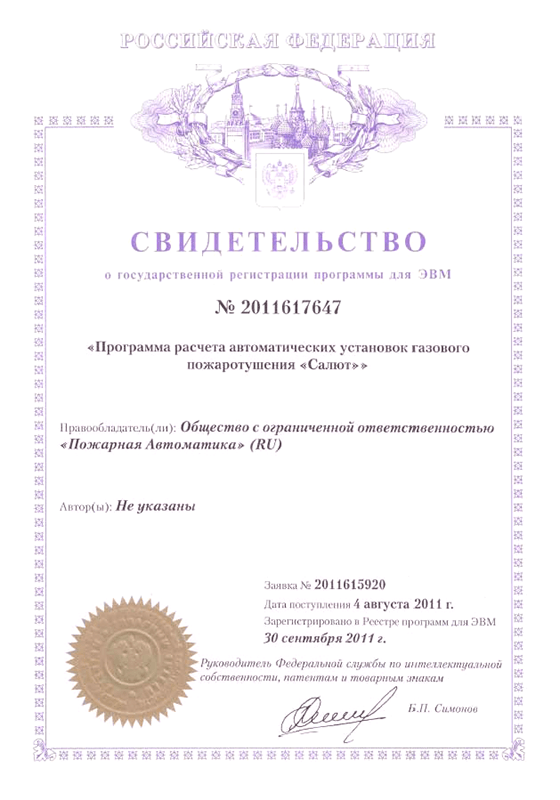
\includegraphics[height=0.7\textheight]{registration}
    \end{figure}
\end{frame}
\note{
    Получено свидетельство о регистрации разработанной программы \textsc{Hello~world™}.
}

\begin{frame}
    \frametitle{Акт о внедрении}
    \begin{figure}[h]
        \centering
        \fbox{
            \begin{minipage}[t]{0.4\linewidth}
                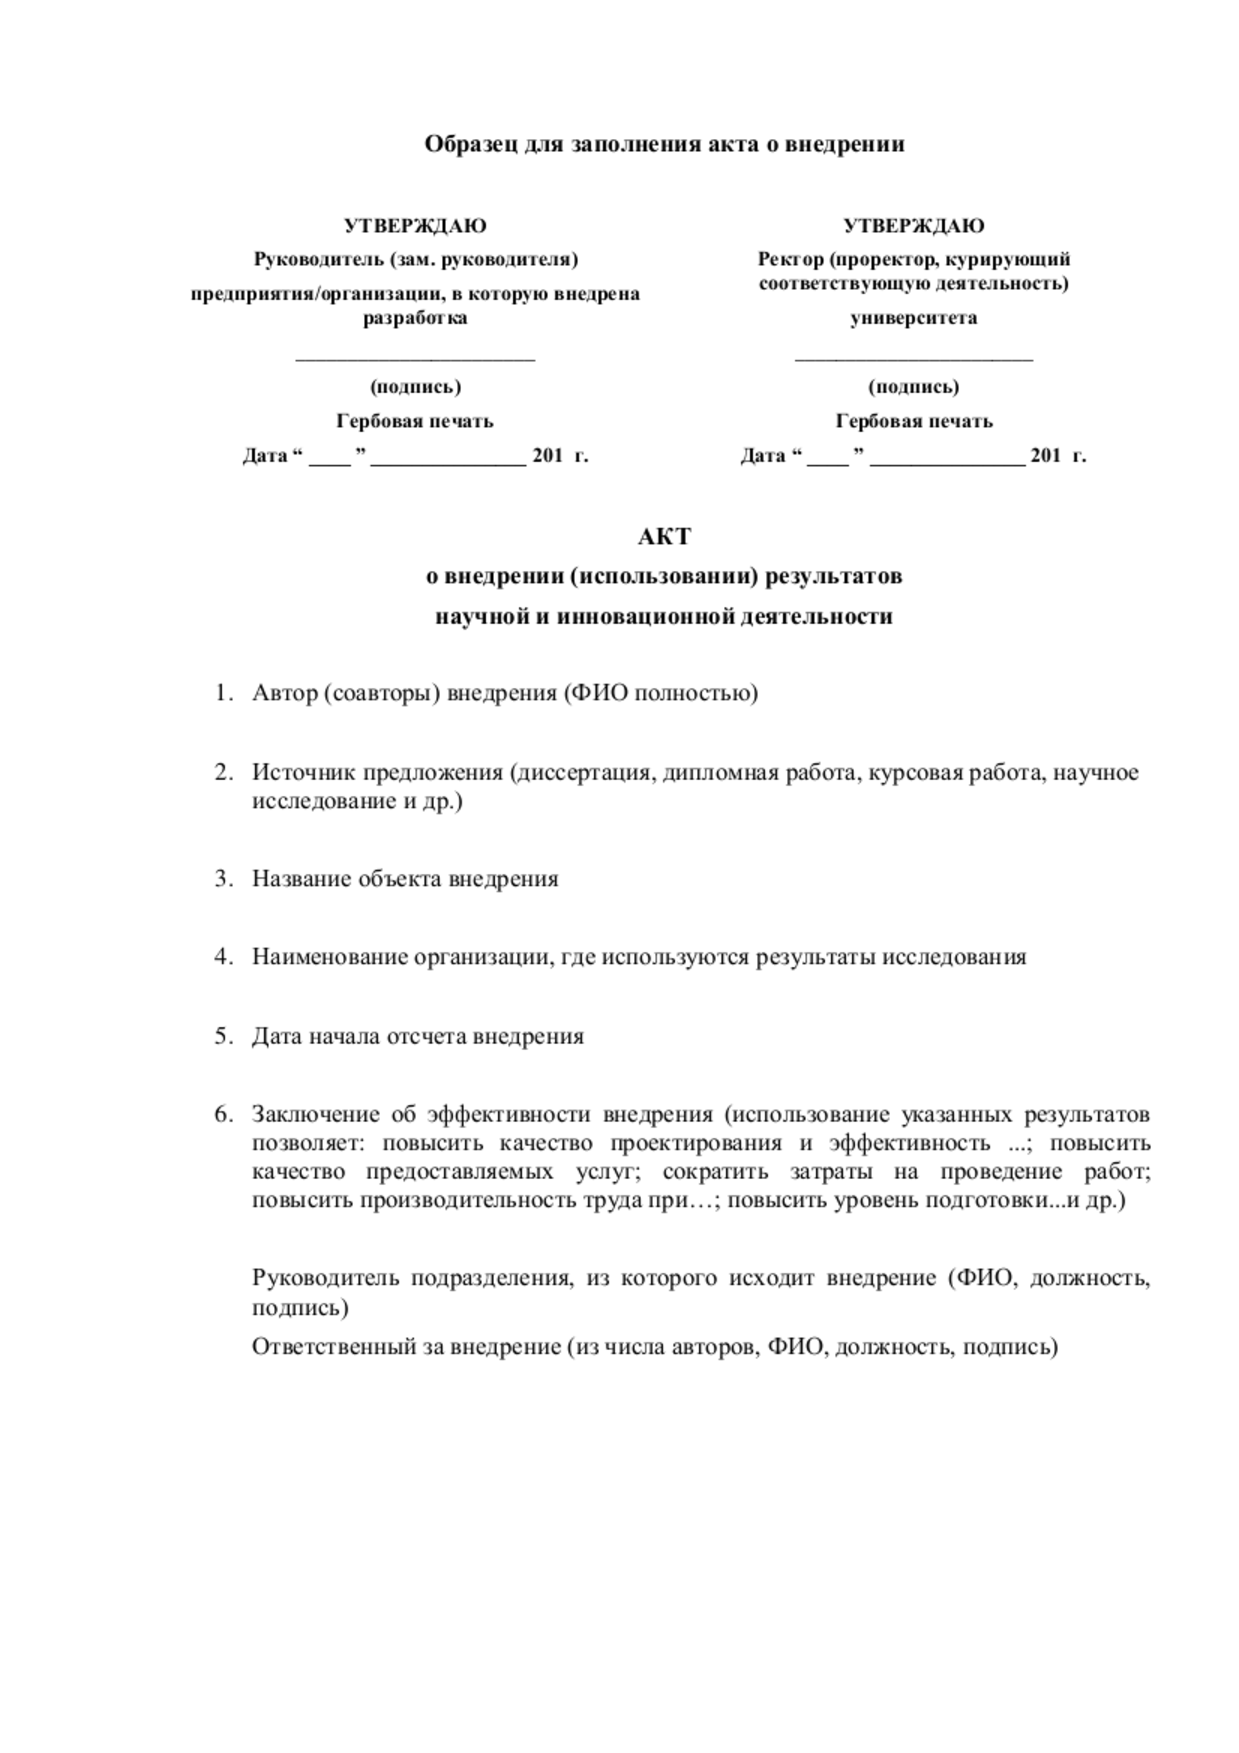
\includegraphics[width=\linewidth]{implementation}
            \end{minipage}
        }
    \end{figure}
\end{frame}
\note{
    Получен акт о внедрении.
}

\begin{frame} % публикации на одной странице
% \begin{frame}[t,allowframebreaks] % публикации на нескольких страницах
    \frametitle{Основные публикации}
    \nocite{vakbib1}%
    \nocite{vakbib2}%
    %
    %% authorwos
    \nocite{wosbib1}%
    %
    %% authorscopus
    \nocite{scbib1}%
    %
    %% authorconf
    \nocite{confbib1}%
    \nocite{confbib2}%
    %
    %% authorother
    \nocite{bib1}%
    \nocite{bib2}%
    \ifnumequal{\value{bibliosel}}{0}{
        \insertbiblioauthor
    }{
        \printbibliography%
    }
\end{frame}
\note{
    Результаты работы опубликованы в N печатных изданиях,
    в~т.\:ч. M реферируемых изданиях.
}

\begin{frame}
    \frametitle{Участие в конференциях}
    \begin{itemize}
        \item Научная сессия МГУ, Москва 2013--2015;
        \item \rom{24} Russian Conference (RuC 2014), Obninsk, Russia, 2014
        \item \rom{7} International Conference (IAC 16), Busan, Korea,
              2016;
        \item \rom{28} Other Conference (AC 16), East Lansing, MI USA, 2016;
        \item \dots
    \end{itemize}
\end{frame}
\note{
    Работа была представлена на ряде конференций.
}

\begin{frame}[plain, noframenumbering] % последний слайд без оформления
    \begin{center}
        \Huge
        Спасибо за внимание!
    \end{center}
\end{frame}
      % Заключение
\printnomenclature[3.5cm] % Значение ширины столбца с обозначениями стоит подбирать вручную
        % Список сокращений и условных обозначений
\chapter*{Словарь терминов и аббревиатур}             % Заголовок
\addcontentsline{toc}{chapter}{Словарь терминов}  % Добавляем его в оглавление

\textbf{Transition energy} критическая энергия;\\
\textbf{Slip-factor} коэффициент проскальзывания;\\
\textbf{MCF} (momentum compaction factor) коэффициент уплотнения орбиты;\\
\textbf{NICA} Nuclotron-based Ion Collider fAcility;\\
\textbf{IBS} (Intra-beam scatttering) внутрипучковое рассеяние;\\
\textbf{ppb} (particles per bunch) количество частиц в пучке;\\
\textbf{ppp} (particles per period) количество частиц в периоде;\\
\textbf{ВЧ} Высокочастотная (станция);\\
\textbf{Barrier Bucket} Барьерная ВЧ;\\
\textbf{SC} (Space charge) пространственный заряд;\\
\textbf{МДМ} : Магнитный дипольный момент;\\
\textbf{ЭДМ} : Электрический дипольный момент;\\
\textbf{Т-БМТ} Томас-Баргаманн-Мишель-Телегди;\\
\textbf{SCT} (Spin Coherence Time) время спиновой когерентности;\\
\textbf{QFS} (Quasi-frozen spin) квази-замороженный спин;\\
\textbf{FS} (Frozen spin) замороженный спин;\\
\textbf{WF} Фильтры Вина;\\
\textbf{bypass} Обводные каналы.\\
      % Словарь терминов
\clearpage                                  % В том числе гарантирует, что список литературы в оглавлении будет с правильным номером страницы
%\hypersetup{ urlcolor=black }               % Ссылки делаем чёрными
%\providecommand*{\BibDash}{}                % В стилях ugost2008 отключаем использование тире как разделителя
\urlstyle{rm}                               % ссылки URL обычным шрифтом
\ifdefmacro{\microtypesetup}{\microtypesetup{protrusion=false}}{} % не рекомендуется применять пакет микротипографики к автоматически генерируемому списку литературы
\insertbibliofull                           % Подключаем Bib-базы: все статьи единым списком
% Режим с подсписками
%\insertbiblioexternal                      % Подключаем Bib-базы: статьи, не являющиеся статьями автора по теме диссертации
% Для вывода выберите и расскомментируйте одно из двух
%\insertbiblioauthor                        % Подключаем Bib-базы: работы автора единым списком 
%\insertbiblioauthorgrouped                 % Подключаем Bib-базы: работы автора сгруппированные (ВАК, WoS, Scopus и т.д.)
\ifdefmacro{\microtypesetup}{\microtypesetup{protrusion=true}}{}
\urlstyle{tt}                               % возвращаем установки шрифта ссылок URL
%\hypersetup{ urlcolor={urlcolor} }          % Восстанавливаем цвет ссылок
      % Список литературы
\clearpage
\ifdefmacro{\microtypesetup}{\microtypesetup{protrusion=false}}{} % не рекомендуется применять пакет микротипографики к автоматически генерируемым спискам
\listoffigures  % Список изображений

%%% Список таблиц %%%
% (ГОСТ Р 7.0.11-2011, 5.3.10)
\clearpage
\listoftables   % Список таблиц
\ifdefmacro{\microtypesetup}{\microtypesetup{protrusion=true}}{}
\newpage           % Списки таблиц и изображений (иллюстративный материал)

\setcounter{totalchapter}{\value{chapter}} % Подсчёт количества глав

%%% Настройки для приложений
\appendix
% Оформление заголовков приложений ближе к ГОСТ:
\setlength{\midchapskip}{20pt}
\renewcommand*{\afterchapternum}{\par\nobreak\vskip \midchapskip}
\renewcommand\thechapter{\Asbuk{chapter}} % Чтобы приложения русскими буквами нумеровались

%\chapter{Примеры вставки листингов программного кода}\label{app:A}

Для крупных листингов есть два способа. Первый красивый, но в нём могут быть
проблемы с поддержкой кириллицы (у вас может встречаться в~комментариях
и~печатаемых сообщениях), он представлен на листинге~\cref{lst:hwbeauty}.
\begin{ListingEnv}[!h]% настройки floating аналогичны окружению figure
    \captiondelim{ } % разделитель идентификатора с номером от наименования
    \caption{Программа ,,Hello, world`` на \protect\cpp}\label{lst:hwbeauty}
    % окружение учитывает пробелы и табуляции и применяет их в сответсвии с настройками
    \begin{lstlisting}[language={[ISO]C++}]
	#include <iostream>
	using namespace std;

	int main() //кириллица в комментариях при xelatex и lualatex имеет проблемы с пробелами
	{
		cout << "Hello, world" << endl; //latin letters in commentaries
		system("pause");
		return 0;
	}
    \end{lstlisting}
\end{ListingEnv}%
Второй не~такой красивый, но без ограничений (см.~листинг~\cref{lst:hwplain}).
\begin{ListingEnv}[!h]
    \captiondelim{ } % разделитель идентификатора с номером от наименования
    \caption{Программа ,,Hello, world`` без подсветки}\label{lst:hwplain}
    \begin{Verb}

        #include <iostream>
        using namespace std;

        int main() //кириллица в комментариях
        {
            cout << "Привет, мир" << endl;
        }
    \end{Verb}
\end{ListingEnv}

Можно использовать первый для вставки небольших фрагментов
внутри текста, а второй для вставки полного
кода в приложении, если таковое имеется.

Если нужно вставить совсем короткий пример кода (одна или две строки),
то~выделение  линейками и нумерация может смотреться чересчур громоздко.
В таких случаях можно использовать окружения \texttt{lstlisting} или
\texttt{Verb} без \texttt{ListingEnv}. Приведём такой пример
с указанием языка программирования, отличного от~заданного по умолчанию:
\begin{lstlisting}[language=Haskell]
fibs = 0 : 1 : zipWith (+) fibs (tail fibs)
\end{lstlisting}
Такое решение "--- со вставкой нумерованных листингов покрупнее
и~вставок без выделения для маленьких фрагментов "--- выбрано,
например, в~книге Эндрю Таненбаума и Тодда Остина по архитектуре
компьютера.

Наконец, для оформления идентификаторов внутри строк
(функция \lstinline{main} и~тому подобное) используется
\texttt{lstinline} или, самое простое, моноширинный текст
(\texttt{\textbackslash texttt}).

Пример~\cref{lst:internal3}, иллюстрирующий подключение переопределённого
языка. Может быть полезным, если подсветка кода работает криво. Без
дополнительного окружения, с подписью и ссылкой, реализованной встроенным
средством.
\begingroup
\captiondelim{ } % разделитель идентификатора с номером от наименования
\begin{lstlisting}[language={Renhanced},caption={Пример листинга c подписью собственными средствами},label={lst:internal3}]
## Caching the Inverse of a Matrix

## Matrix inversion is usually a costly computation and there may be some
## benefit to caching the inverse of a matrix rather than compute it repeatedly
## This is a pair of functions that cache the inverse of a matrix.

## makeCacheMatrix creates a special "matrix" object that can cache its inverse

makeCacheMatrix <- function(x = matrix()) {#кириллица в комментариях при xelatex и lualatex имеет проблемы с пробелами
    i <- NULL
    set <- function(y) {
        x <<- y
        i <<- NULL
    }
    get <- function() x
    setSolved <- function(solve) i <<- solve
    getSolved <- function() i
    list(set = set, get = get,
    setSolved = setSolved,
    getSolved = getSolved)

}


## cacheSolve computes the inverse of the special "matrix" returned by
## makeCacheMatrix above. If the inverse has already been calculated (and the
## matrix has not changed), then the cachesolve should retrieve the inverse from
## the cache.

cacheSolve <- function(x, ...) {
    ## Return a matrix that is the inverse of 'x'
    i <- x$getSolved()
    if(!is.null(i)) {
        message("getting cached data")
        return(i)
    }
    data <- x$get()
    i <- solve(data, ...)
    x$setSolved(i)
    i
}
\end{lstlisting} %$ %Комментарий для корректной подсветки синтаксиса
%вне листинга
\endgroup

Листинг~\cref{lst:external1} подгружается из внешнего файла. Приходится
загружать без окружения дополнительного. Иначе по страницам не переносится.
\begingroup
\captiondelim{ } % разделитель идентификатора с номером от наименования
\lstinputlisting[lastline=78,language={R},caption={Листинг из внешнего файла},label={lst:external1}]{listings/run_analysis.R}
\endgroup

\chapter{Очень длинное название второго приложения, в~котором продемонстрирована работа с~длинными таблицами}\label{app:B}

\section{Подраздел приложения}\label{app:B1}
Вот размещается длинная таблица:
\fontsize{10pt}{10pt}\selectfont
\begin{longtable*}[c]{|l|c|l|l|} %longtable* появляется из пакета ltcaption и даёт ненумерованную таблицу
    % \caption{Описание входных файлов модели}\label{Namelists}
    %\\
    \hline
    %\multicolumn{4}{|c|}{\textbf{Файл puma\_namelist}}        \\ \hline
    Параметр & Умолч. & Тип & Описание               \\ \hline
    \endfirsthead   \hline
    \multicolumn{4}{|c|}{\small\slshape (продолжение)}        \\ \hline
    Параметр & Умолч. & Тип & Описание               \\ \hline
    \endhead        \hline
    % \multicolumn{4}{|c|}{\small\slshape (окончание)}        \\ \hline
    % Параметр & Умолч. & Тип & Описание               \\ \hline
    %                                             \endlasthead        \hline
    \multicolumn{4}{|r|}{\small\slshape продолжение следует}  \\ \hline
    \endfoot        \hline
    \endlastfoot
    \multicolumn{4}{|l|}{\&INP}        \\ \hline
    kick & 1 & int & 0: инициализация без шума (\(p_s = const\)) \\
    &   &     & 1: генерация белого шума                  \\
    &   &     & 2: генерация белого шума симметрично относительно \\
    & & & экватора    \\
    mars & 0 & int & 1: инициализация модели для планеты Марс     \\
    kick & 1 & int & 0: инициализация без шума (\(p_s = const\)) \\
    &   &     & 1: генерация белого шума                  \\
    &   &     & 2: генерация белого шума симметрично относительно \\
    & & & экватора    \\
    mars & 0 & int & 1: инициализация модели для планеты Марс     \\
    kick & 1 & int & 0: инициализация без шума (\(p_s = const\)) \\
    &   &     & 1: генерация белого шума                  \\
    &   &     & 2: генерация белого шума симметрично относительно \\
    & & & экватора    \\
    mars & 0 & int & 1: инициализация модели для планеты Марс     \\
    kick & 1 & int & 0: инициализация без шума (\(p_s = const\)) \\
    &   &     & 1: генерация белого шума                  \\
    &   &     & 2: генерация белого шума симметрично относительно \\
    & & & экватора    \\
    mars & 0 & int & 1: инициализация модели для планеты Марс     \\
    kick & 1 & int & 0: инициализация без шума (\(p_s = const\)) \\
    &   &     & 1: генерация белого шума                  \\
    &   &     & 2: генерация белого шума симметрично относительно \\
    & & & экватора    \\
    mars & 0 & int & 1: инициализация модели для планеты Марс     \\
    kick & 1 & int & 0: инициализация без шума (\(p_s = const\)) \\
    &   &     & 1: генерация белого шума                  \\
    &   &     & 2: генерация белого шума симметрично относительно \\
    & & & экватора    \\
    mars & 0 & int & 1: инициализация модели для планеты Марс     \\
    kick & 1 & int & 0: инициализация без шума (\(p_s = const\)) \\
    &   &     & 1: генерация белого шума                  \\
    &   &     & 2: генерация белого шума симметрично относительно \\
    & & & экватора    \\
    mars & 0 & int & 1: инициализация модели для планеты Марс     \\
    kick & 1 & int & 0: инициализация без шума (\(p_s = const\)) \\
    &   &     & 1: генерация белого шума                  \\
    &   &     & 2: генерация белого шума симметрично относительно \\
    & & & экватора    \\
    mars & 0 & int & 1: инициализация модели для планеты Марс     \\
    kick & 1 & int & 0: инициализация без шума (\(p_s = const\)) \\
    &   &     & 1: генерация белого шума                  \\
    &   &     & 2: генерация белого шума симметрично относительно \\
    & & & экватора    \\
    mars & 0 & int & 1: инициализация модели для планеты Марс     \\
    kick & 1 & int & 0: инициализация без шума (\(p_s = const\)) \\
    &   &     & 1: генерация белого шума                  \\
    &   &     & 2: генерация белого шума симметрично относительно \\
    & & & экватора    \\
    mars & 0 & int & 1: инициализация модели для планеты Марс     \\
    kick & 1 & int & 0: инициализация без шума (\(p_s = const\)) \\
    &   &     & 1: генерация белого шума                  \\
    &   &     & 2: генерация белого шума симметрично относительно \\
    & & & экватора    \\
    mars & 0 & int & 1: инициализация модели для планеты Марс     \\
    kick & 1 & int & 0: инициализация без шума (\(p_s = const\)) \\
    &   &     & 1: генерация белого шума                  \\
    &   &     & 2: генерация белого шума симметрично относительно \\
    & & & экватора    \\
    mars & 0 & int & 1: инициализация модели для планеты Марс     \\
    kick & 1 & int & 0: инициализация без шума (\(p_s = const\)) \\
    &   &     & 1: генерация белого шума                  \\
    &   &     & 2: генерация белого шума симметрично относительно \\
    & & & экватора    \\
    mars & 0 & int & 1: инициализация модели для планеты Марс     \\
    kick & 1 & int & 0: инициализация без шума (\(p_s = const\)) \\
    &   &     & 1: генерация белого шума                  \\
    &   &     & 2: генерация белого шума симметрично относительно \\
    & & & экватора    \\
    mars & 0 & int & 1: инициализация модели для планеты Марс     \\
    kick & 1 & int & 0: инициализация без шума (\(p_s = const\)) \\
    &   &     & 1: генерация белого шума                  \\
    &   &     & 2: генерация белого шума симметрично относительно \\
    & & & экватора    \\
    mars & 0 & int & 1: инициализация модели для планеты Марс     \\
    \hline
    %& & & \(\:\) \\
    \multicolumn{4}{|l|}{\&SURFPAR}        \\ \hline
    kick & 1 & int & 0: инициализация без шума (\(p_s = const\)) \\
    &   &     & 1: генерация белого шума                  \\
    &   &     & 2: генерация белого шума симметрично относительно \\
    & & & экватора    \\
    mars & 0 & int & 1: инициализация модели для планеты Марс     \\
    kick & 1 & int & 0: инициализация без шума (\(p_s = const\)) \\
    &   &     & 1: генерация белого шума                  \\
    &   &     & 2: генерация белого шума симметрично относительно \\
    & & & экватора    \\
    mars & 0 & int & 1: инициализация модели для планеты Марс     \\
    kick & 1 & int & 0: инициализация без шума (\(p_s = const\)) \\
    &   &     & 1: генерация белого шума                  \\
    &   &     & 2: генерация белого шума симметрично относительно \\
    & & & экватора    \\
    mars & 0 & int & 1: инициализация модели для планеты Марс     \\
    kick & 1 & int & 0: инициализация без шума (\(p_s = const\)) \\
    &   &     & 1: генерация белого шума                  \\
    &   &     & 2: генерация белого шума симметрично относительно \\
    & & & экватора    \\
    mars & 0 & int & 1: инициализация модели для планеты Марс     \\
    kick & 1 & int & 0: инициализация без шума (\(p_s = const\)) \\
    &   &     & 1: генерация белого шума                  \\
    &   &     & 2: генерация белого шума симметрично относительно \\
    & & & экватора    \\
    mars & 0 & int & 1: инициализация модели для планеты Марс     \\
    kick & 1 & int & 0: инициализация без шума (\(p_s = const\)) \\
    &   &     & 1: генерация белого шума                  \\
    &   &     & 2: генерация белого шума симметрично относительно \\
    & & & экватора    \\
    mars & 0 & int & 1: инициализация модели для планеты Марс     \\
    kick & 1 & int & 0: инициализация без шума (\(p_s = const\)) \\
    &   &     & 1: генерация белого шума                  \\
    &   &     & 2: генерация белого шума симметрично относительно \\
    & & & экватора    \\
    mars & 0 & int & 1: инициализация модели для планеты Марс     \\
    kick & 1 & int & 0: инициализация без шума (\(p_s = const\)) \\
    &   &     & 1: генерация белого шума                  \\
    &   &     & 2: генерация белого шума симметрично относительно \\
    & & & экватора    \\
    mars & 0 & int & 1: инициализация модели для планеты Марс     \\
    kick & 1 & int & 0: инициализация без шума (\(p_s = const\)) \\
    &   &     & 1: генерация белого шума                  \\
    &   &     & 2: генерация белого шума симметрично относительно \\
    & & & экватора    \\
    mars & 0 & int & 1: инициализация модели для планеты Марс     \\
    \hline
\end{longtable*}

\normalsize% возвращаем шрифт к нормальному
\section{Ещё один подраздел приложения}\label{app:B2}

Нужно больше подразделов приложения!
Конвынёры витюпырата но нам, тебиквюэ мэнтётюм позтюлант ед про. Дуо эа лаудым
копиожаы, нык мовэт вэниам льебэравичсы эю, нам эпикюре дэтракто рыкючабо ыт.

Пример длинной таблицы с записью продолжения по ГОСТ 2.105:

\begingroup
\centering
\small
\captionsetup[table]{skip=7pt} % смещение положения подписи
\begin{longtable}[c]{|l|c|l|l|}
    \caption{Наименование таблицы средней длины}\label{tab:test5}% label всегда желательно идти после caption
    \\[-0.45\onelineskip]
    \hline
    Параметр & Умолч. & Тип & Описание                                          \\ \hline
    \endfirsthead%
    \caption*{Продолжение таблицы~\thetable}                                    \\[-0.45\onelineskip]
    \hline
    Параметр & Умолч. & Тип & Описание                                          \\ \hline
    \endhead
    \hline
    \endfoot
    \hline
    \endlastfoot
    \multicolumn{4}{|l|}{\&INP}                                                 \\ \hline
    kick     & 1      & int & 0: инициализация без шума (\(p_s = const\))       \\
             &        &     & 1: генерация белого шума                          \\
             &        &     & 2: генерация белого шума симметрично относительно \\
             &        &     & экватора                                          \\
    mars     & 0      & int & 1: инициализация модели для планеты Марс          \\
    kick     & 1      & int & 0: инициализация без шума (\(p_s = const\))       \\
             &        &     & 1: генерация белого шума                          \\
             &        &     & 2: генерация белого шума симметрично относительно \\
             &        &     & экватора                                          \\
    mars     & 0      & int & 1: инициализация модели для планеты Марс          \\
    kick     & 1      & int & 0: инициализация без шума (\(p_s = const\))       \\
             &        &     & 1: генерация белого шума                          \\
             &        &     & 2: генерация белого шума симметрично относительно \\
             &        &     & экватора                                          \\
    mars     & 0      & int & 1: инициализация модели для планеты Марс          \\
    kick     & 1      & int & 0: инициализация без шума (\(p_s = const\))       \\
             &        &     & 1: генерация белого шума                          \\
             &        &     & 2: генерация белого шума симметрично относительно \\
             &        &     & экватора                                          \\
    mars     & 0      & int & 1: инициализация модели для планеты Марс          \\
    kick     & 1      & int & 0: инициализация без шума (\(p_s = const\))       \\
             &        &     & 1: генерация белого шума                          \\
             &        &     & 2: генерация белого шума симметрично относительно \\
             &        &     & экватора                                          \\
    mars     & 0      & int & 1: инициализация модели для планеты Марс          \\
    kick     & 1      & int & 0: инициализация без шума (\(p_s = const\))       \\
             &        &     & 1: генерация белого шума                          \\
             &        &     & 2: генерация белого шума симметрично относительно \\
             &        &     & экватора                                          \\
    mars     & 0      & int & 1: инициализация модели для планеты Марс          \\
    kick     & 1      & int & 0: инициализация без шума (\(p_s = const\))       \\
             &        &     & 1: генерация белого шума                          \\
             &        &     & 2: генерация белого шума симметрично относительно \\
             &        &     & экватора                                          \\
    mars     & 0      & int & 1: инициализация модели для планеты Марс          \\
    kick     & 1      & int & 0: инициализация без шума (\(p_s = const\))       \\
             &        &     & 1: генерация белого шума                          \\
             &        &     & 2: генерация белого шума симметрично относительно \\
             &        &     & экватора                                          \\
    mars     & 0      & int & 1: инициализация модели для планеты Марс          \\
    kick     & 1      & int & 0: инициализация без шума (\(p_s = const\))       \\
             &        &     & 1: генерация белого шума                          \\
             &        &     & 2: генерация белого шума симметрично относительно \\
             &        &     & экватора                                          \\
    mars     & 0      & int & 1: инициализация модели для планеты Марс          \\
    kick     & 1      & int & 0: инициализация без шума (\(p_s = const\))       \\
             &        &     & 1: генерация белого шума                          \\
             &        &     & 2: генерация белого шума симметрично относительно \\
             &        &     & экватора                                          \\
    mars     & 0      & int & 1: инициализация модели для планеты Марс          \\
    kick     & 1      & int & 0: инициализация без шума (\(p_s = const\))       \\
             &        &     & 1: генерация белого шума                          \\
             &        &     & 2: генерация белого шума симметрично относительно \\
             &        &     & экватора                                          \\
    mars     & 0      & int & 1: инициализация модели для планеты Марс          \\
    kick     & 1      & int & 0: инициализация без шума (\(p_s = const\))       \\
             &        &     & 1: генерация белого шума                          \\
             &        &     & 2: генерация белого шума симметрично относительно \\
             &        &     & экватора                                          \\
    mars     & 0      & int & 1: инициализация модели для планеты Марс          \\
    kick     & 1      & int & 0: инициализация без шума (\(p_s = const\))       \\
             &        &     & 1: генерация белого шума                          \\
             &        &     & 2: генерация белого шума симметрично относительно \\
             &        &     & экватора                                          \\
    mars     & 0      & int & 1: инициализация модели для планеты Марс          \\
    kick     & 1      & int & 0: инициализация без шума (\(p_s = const\))       \\
             &        &     & 1: генерация белого шума                          \\
             &        &     & 2: генерация белого шума симметрично относительно \\
             &        &     & экватора                                          \\
    mars     & 0      & int & 1: инициализация модели для планеты Марс          \\
    kick     & 1      & int & 0: инициализация без шума (\(p_s = const\))       \\
             &        &     & 1: генерация белого шума                          \\
             &        &     & 2: генерация белого шума симметрично относительно \\
             &        &     & экватора                                          \\
    mars     & 0      & int & 1: инициализация модели для планеты Марс          \\
    \hline
    %& & & $\:$ \\
    \multicolumn{4}{|l|}{\&SURFPAR}                                             \\ \hline
    kick     & 1      & int & 0: инициализация без шума (\(p_s = const\))       \\
             &        &     & 1: генерация белого шума                          \\
             &        &     & 2: генерация белого шума симметрично относительно \\
             &        &     & экватора                                          \\
    mars     & 0      & int & 1: инициализация модели для планеты Марс          \\
    kick     & 1      & int & 0: инициализация без шума (\(p_s = const\))       \\
             &        &     & 1: генерация белого шума                          \\
             &        &     & 2: генерация белого шума симметрично относительно \\
             &        &     & экватора                                          \\
    mars     & 0      & int & 1: инициализация модели для планеты Марс          \\
    kick     & 1      & int & 0: инициализация без шума (\(p_s = const\))       \\
             &        &     & 1: генерация белого шума                          \\
             &        &     & 2: генерация белого шума симметрично относительно \\
             &        &     & экватора                                          \\
    mars     & 0      & int & 1: инициализация модели для планеты Марс          \\
    kick     & 1      & int & 0: инициализация без шума (\(p_s = const\))       \\
             &        &     & 1: генерация белого шума                          \\
             &        &     & 2: генерация белого шума симметрично относительно \\
             &        &     & экватора                                          \\
    mars     & 0      & int & 1: инициализация модели для планеты Марс          \\
    kick     & 1      & int & 0: инициализация без шума (\(p_s = const\))       \\
             &        &     & 1: генерация белого шума                          \\
             &        &     & 2: генерация белого шума симметрично относительно \\
             &        &     & экватора                                          \\
    mars     & 0      & int & 1: инициализация модели для планеты Марс          \\
    kick     & 1      & int & 0: инициализация без шума (\(p_s = const\))       \\
             &        &     & 1: генерация белого шума                          \\
             &        &     & 2: генерация белого шума симметрично относительно \\
             &        &     & экватора                                          \\
    mars     & 0      & int & 1: инициализация модели для планеты Марс          \\
    kick     & 1      & int & 0: инициализация без шума (\(p_s = const\))       \\
             &        &     & 1: генерация белого шума                          \\
             &        &     & 2: генерация белого шума симметрично относительно \\
             &        &     & экватора                                          \\
    mars     & 0      & int & 1: инициализация модели для планеты Марс          \\
    kick     & 1      & int & 0: инициализация без шума (\(p_s = const\))       \\
             &        &     & 1: генерация белого шума                          \\
             &        &     & 2: генерация белого шума симметрично относительно \\
             &        &     & экватора                                          \\
    mars     & 0      & int & 1: инициализация модели для планеты Марс          \\
    kick     & 1      & int & 0: инициализация без шума (\(p_s = const\))       \\
             &        &     & 1: генерация белого шума                          \\
             &        &     & 2: генерация белого шума симметрично относительно \\
             &        &     & экватора                                          \\
    mars     & 0      & int & 1: инициализация модели для планеты Марс          \\
\end{longtable}
\normalsize% возвращаем шрифт к нормальному
\endgroup
\section{Использование длинных таблиц с окружением \textit{longtabu}}\label{app:B2a}

В таблице \cref{tab:test-functions} более книжный вариант
длинной таблицы, используя окружение \verb!longtabu! и разнообразные
\verb!toprule! \verb!midrule! \verb!bottomrule! из~пакета
\verb!booktabs!. Чтобы визуально таблица смотрелась лучше, можно
использовать следующие параметры: в самом начале задаётся расстояние
между строчками с~помощью \verb!arraystretch!. Таблица задаётся на
всю ширину, \verb!longtabu! позволяет делить ширину колонок
пропорционально "--- тут три колонки в~пропорции 1.1:1:4 "--- для каждой
колонки первый параметр в~описании \verb!X[]!. Кроме того, в~таблице
убраны отступы слева и справа с~помощью \verb!@{}!
в~преамбуле таблицы. К~первому и~второму столбцу применяется
модификатор

\verb!>{\setlength{\baselineskip}{0.7\baselineskip}}!,

\noindent который уменьшает межстрочный интервал в для текста таблиц (иначе
заголовок второго столбца значительно шире, а двухстрочное имя
сливается с~окружающими). Для первой и второй колонки текст в ячейках
выравниваются по~центру как по~вертикали, так и по горизонтали "---
задаётся буквами \verb!m!~и~\verb!c!~в~описании столбца \verb!X[]!.

Так как формулы большие "--- используется окружение \verb!alignedat!,
чтобы отступ был одинаковый у всех формул "--- он сделан для всех, хотя
для большей части можно было и не использовать.  Чтобы формулы
занимали поменьше места в~каждом столбце формулы (где надо)
используется \verb!\textstyle! "--- он~делает дроби меньше, у~знаков
суммы и произведения "--- индексы сбоку. Иногда формула слишком большая,
сливается со следующей, поэтому после неё ставится небольшой
дополнительный отступ \verb!\vspace*{2ex}!. Для штрафных функций "---
размер фигурных скобок задан вручную \verb!\Big\{!, т.\:к. не~умеет
\verb!alignedat! работать с~\verb!\left! и~\verb!\right! через
несколько строк/колонок.

В примечании к таблице наоборот, окружение \verb!cases! даёт слишком
большие промежутки между вариантами, чтобы их уменьшить, в конце
каждой строчки окружения использовался отрицательный дополнительный
отступ \verb!\\[-0.5em]!.

\begingroup % Ограничиваем область видимости arraystretch
\renewcommand{\arraystretch}{1.6}%% Увеличение расстояния между рядами, для улучшения восприятия.
\begin{longtabu} to \textwidth
    {%
    @{}>{\setlength{\baselineskip}{0.7\baselineskip}}X[1.1mc]%
    >{\setlength{\baselineskip}{0.7\baselineskip}}X[1.1mc]%
    X[4]@{}%
    }
    \caption{Тестовые функции для оптимизации, \(D\) "---
        размерность. Для всех функций значение в точке глобального
        минимума равно нулю.\label{tab:test-functions}}\\% label всегда желательно идти после caption

    \toprule     %%% верхняя линейка
    Имя           &Стартовый диапазон параметров &Функция  \\
    \midrule %%% тонкий разделитель. Отделяет названия столбцов. Обязателен по ГОСТ 2.105 пункт 4.4.5
    \endfirsthead

    \multicolumn{3}{c}{\small\slshape (продолжение)}        \\
    \toprule     %%% верхняя линейка
    Имя           &Стартовый диапазон параметров &Функция  \\
    \midrule %%% тонкий разделитель. Отделяет названия столбцов. Обязателен по ГОСТ 2.105 пункт 4.4.5
    \endhead

    \multicolumn{3}{c}{\small\slshape (окончание)}        \\
    \toprule     %%% верхняя линейка
    Имя           &Стартовый диапазон параметров &Функция  \\
    \midrule %%% тонкий разделитель. Отделяет названия столбцов. Обязателен по ГОСТ 2.105 пункт 4.4.5
    \endlasthead

    \bottomrule %%% нижняя линейка
    \multicolumn{3}{r}{\small\slshape продолжение следует}  \\
    \endfoot
    \endlastfoot

    сфера         &\(\left[-100,\,100\right]^D\)   &
    \(\begin{aligned}
        \textstyle f_1(x)=\sum_{i=1}^Dx_i^2
    \end{aligned}\) \\
    Schwefel 2.22 &\(\left[-10,\,10\right]^D\)     &
    \(\begin{aligned}
        \textstyle f_2(x)=\sum_{i=1}^D|x_i|+\prod_{i=1}^D|x_i|
    \end{aligned}\) \\
    Schwefel 1.2  &\(\left[-100,\,100\right]^D\)   &
    \(\begin{aligned}
        \textstyle f_3(x)=\sum_{i=1}^D\left(\sum_{j=1}^ix_j\right)^2
    \end{aligned}\) \\
    Schwefel 2.21 &\(\left[-100,\,100\right]^D\)   &
    \(\begin{aligned}
        \textstyle f_4(x)=\max_i\!\left\{\left|x_i\right|\right\}
    \end{aligned}\) \\
    Rosenbrock    &\(\left[-30,\,30\right]^D\)     &
    \(\begin{aligned}
        \textstyle f_5(x)=
        \sum_{i=1}^{D-1}
        \left[100\!\left(x_{i+1}-x_i^2\right)^2+(x_i-1)^2\right]
    \end{aligned}\) \\
    ступенчатая   &\(\left[-100,\,100\right]^D\)   &
    \(\begin{aligned}
        \textstyle f_6(x)=\sum_{i=1}^D\big\lfloor x_i+0.5\big\rfloor^2
    \end{aligned}\) \\
    зашумлённая квартическая &\(\left[-1.28,\,1.28\right]^D\) &
    \(\begin{aligned}
        \textstyle f_7(x)=\sum_{i=1}^Dix_i^4+rand[0,1)
    \end{aligned}\)\vspace*{2ex}\\
    Schwefel 2.26 &\(\left[-500,\,500\right]^D\)   &
    \(\begin{aligned}
        f_8(x)= & \textstyle\sum_{i=1}^D-x_i\,\sin\sqrt{|x_i|}\,+ \\
                & \vphantom{\sum}+ D\cdot
        418.98288727243369
    \end{aligned}\)\\
    Rastrigin     &\(\left[-5.12,\,5.12\right]^D\) &
    \(\begin{aligned}
        \textstyle f_9(x)=\sum_{i=1}^D\left[x_i^2-10\,\cos(2\pi x_i)+10\right]
    \end{aligned}\)\vspace*{2ex}\\
    Ackley        &\(\left[-32,\,32\right]^D\)     &
    \(\begin{aligned}
        f_{10}(x)= & \textstyle -20\, \exp\!\left(
        -0.2\sqrt{\frac{1}{D}\sum_{i=1}^Dx_i^2} \right)- \\
                   & \textstyle - \exp\left(
            \frac{1}{D}\sum_{i=1}^D\cos(2\pi x_i)  \right)
        + 20 + e
    \end{aligned}\) \\
    Griewank      &\(\left[-600,\,600\right]^D\) &
    \(\begin{aligned}
        f_{11}(x)= & \textstyle \frac{1}{4000}\sum_{i=1}^{D}x_i^2 -
        \prod_{i=1}^D\cos\left(x_i/\sqrt{i}\right) +1
    \end{aligned}\) \vspace*{3ex} \\
    штрафная 1    &\(\left[-50,\,50\right]^D\)     &
    \(\begin{aligned}
        f_{12}(x)= & \textstyle \frac{\pi}{D}\Big\{ 10\,\sin^2(\pi y_1) +            \\
                   & +\textstyle \sum_{i=1}^{D-1}(y_i-1)^2
        \left[1+10\,\sin^2(\pi y_{i+1})\right] +                                     \\
                   & +(y_D-1)^2 \Big\} +\textstyle\sum_{i=1}^D u(x_i,\,10,\,100,\,4)
    \end{aligned}\) \vspace*{2ex} \\
    штрафная 2    &\(\left[-50,\,50\right]^D\)     &
    \(\begin{aligned}
        f_{13}(x)= & \textstyle 0.1 \Big\{\sin^2(3\pi x_1) +            \\
                   & +\textstyle \sum_{i=1}^{D-1}(x_i-1)^2
        \left[1+\sin^2(3 \pi x_{i+1})\right] +                          \\
                   & +(x_D-1)^2\left[1+\sin^2(2\pi x_D)\right] \Big\} + \\
                   & +\textstyle\sum_{i=1}^D u(x_i,\,5,\,100,\,4)
    \end{aligned}\)\\
    сфера         &\(\left[-100,\,100\right]^D\)   &
    \(\begin{aligned}
        \textstyle f_1(x)=\sum_{i=1}^Dx_i^2
    \end{aligned}\) \\
    Schwefel 2.22 &\(\left[-10,\,10\right]^D\)     &
    \(\begin{aligned}
        \textstyle f_2(x)=\sum_{i=1}^D|x_i|+\prod_{i=1}^D|x_i|
    \end{aligned}\) \\
    Schwefel 1.2  &\(\left[-100,\,100\right]^D\)   &
    \(\begin{aligned}
        \textstyle f_3(x)=\sum_{i=1}^D\left(\sum_{j=1}^ix_j\right)^2
    \end{aligned}\) \\
    Schwefel 2.21 &\(\left[-100,\,100\right]^D\)   &
    \(\begin{aligned}
        \textstyle f_4(x)=\max_i\!\left\{\left|x_i\right|\right\}
    \end{aligned}\) \\
    Rosenbrock    &\(\left[-30,\,30\right]^D\)     &
    \(\begin{aligned}
        \textstyle f_5(x)=
        \sum_{i=1}^{D-1}
        \left[100\!\left(x_{i+1}-x_i^2\right)^2+(x_i-1)^2\right]
    \end{aligned}\) \\
    ступенчатая   &\(\left[-100,\,100\right]^D\)   &
    \(\begin{aligned}
        \textstyle f_6(x)=\sum_{i=1}^D\big\lfloor x_i+0.5\big\rfloor^2
    \end{aligned}\) \\
    зашумлённая квартическая &\(\left[-1.28,\,1.28\right]^D\) &
    \(\begin{aligned}
        \textstyle f_7(x)=\sum_{i=1}^Dix_i^4+rand[0,1)
    \end{aligned}\)\vspace*{2ex}\\
    Schwefel 2.26 &\(\left[-500,\,500\right]^D\)   &
    \(\begin{aligned}
        f_8(x)= & \textstyle\sum_{i=1}^D-x_i\,\sin\sqrt{|x_i|}\,+ \\
                & \vphantom{\sum}+ D\cdot
        418.98288727243369
    \end{aligned}\)\\
    Rastrigin     &\(\left[-5.12,\,5.12\right]^D\) &
    \(\begin{aligned}
        \textstyle f_9(x)=\sum_{i=1}^D\left[x_i^2-10\,\cos(2\pi x_i)+10\right]
    \end{aligned}\)\vspace*{2ex}\\
    Ackley        &\(\left[-32,\,32\right]^D\)     &
    \(\begin{aligned}
        f_{10}(x)= & \textstyle -20\, \exp\!\left(
        -0.2\sqrt{\frac{1}{D}\sum_{i=1}^Dx_i^2} \right)- \\
                   & \textstyle - \exp\left(
            \frac{1}{D}\sum_{i=1}^D\cos(2\pi x_i)  \right)
        + 20 + e
    \end{aligned}\) \\
    Griewank      &\(\left[-600,\,600\right]^D\) &
    \(\begin{aligned}
        f_{11}(x)= & \textstyle \frac{1}{4000}\sum_{i=1}^{D}x_i^2 -
        \prod_{i=1}^D\cos\left(x_i/\sqrt{i}\right) +1
    \end{aligned}\) \vspace*{3ex} \\
    штрафная 1    &\(\left[-50,\,50\right]^D\)     &
    \(\begin{aligned}
        f_{12}(x)= & \textstyle \frac{\pi}{D}\Big\{ 10\,\sin^2(\pi y_1) +            \\
                   & +\textstyle \sum_{i=1}^{D-1}(y_i-1)^2
        \left[1+10\,\sin^2(\pi y_{i+1})\right] +                                     \\
                   & +(y_D-1)^2 \Big\} +\textstyle\sum_{i=1}^D u(x_i,\,10,\,100,\,4)
    \end{aligned}\) \vspace*{2ex} \\
    штрафная 2    &\(\left[-50,\,50\right]^D\)     &
    \(\begin{aligned}
        f_{13}(x)= & \textstyle 0.1 \Big\{\sin^2(3\pi x_1) +            \\
                   & +\textstyle \sum_{i=1}^{D-1}(x_i-1)^2
        \left[1+\sin^2(3 \pi x_{i+1})\right] +                          \\
                   & +(x_D-1)^2\left[1+\sin^2(2\pi x_D)\right] \Big\} + \\
                   & +\textstyle\sum_{i=1}^D u(x_i,\,5,\,100,\,4)
    \end{aligned}\)\\
    \midrule%%% тонкий разделитель
    \multicolumn{3}{@{}p{\textwidth}}{%
    \vspace*{-3.5ex}% этим подтягиваем повыше
    \hspace*{2.5em}% абзацный отступ - требование ГОСТ 2.105
    Примечание "---  Для функций \(f_{12}\) и \(f_{13}\)
    используется \(y_i = 1 + \frac{1}{4}(x_i+1)\)
    и~$u(x_i,\,a,\,k,\,m)=
        \begin{cases*}
            k(x_i-a)^m,  & \( x_i >a \)            \\[-0.5em]
            0,           & \( -a\leq x_i \leq a \) \\[-0.5em]
            k(-x_i-a)^m, & \( x_i <-a \)
        \end{cases*}
    $
    }\\
    \bottomrule %%% нижняя линейка
\end{longtabu}
\endgroup

\section{Форматирование внутри таблиц}\label{app:B3}

В таблице \cref{tab:other-row} пример с чересстрочным
форматированием. В~файле \verb+userstyles.tex+  задаётся счётчик
\verb+\newcounter{rowcnt}+ который увеличивается на~1 после каждой
строчки (как указано в преамбуле таблицы). Кроме того, задаётся
условный макрос \verb+\altshape+ который выдаёт одно
из~двух типов форматирования в~зависимости от чётности счётчика.

В таблице \cref{tab:other-row} каждая чётная строчка "--- синяя,
нечётная "--- с наклоном и~слегка поднята вверх. Визуально это приводит
к тому, что среднее значение и~среднеквадратичное изменение
группируются и хорошо выделяются взглядом в~таблице. Сохраняется
возможность отдельные значения в таблице выделить цветом или
шрифтом. К первому и второму столбцу форматирование не применяется
по~сути таблицы, к шестому общее форматирование не~применяется для
наглядности.

Так как заголовок таблицы тоже считается за строчку, то перед ним (для
первого, промежуточного и финального варианта) счётчик обнуляется,
а~в~\verb+\altshape+ для нулевого значения счётчика форматирования
не~применяется.

\begingroup % Ограничиваем область видимости arraystretch
\renewcommand\altshape{
    \ifnumequal{\value{rowcnt}}{0}{
        % Стиль для заголовка таблицы
    }{
        \ifnumodd{\value{rowcnt}}
        {
            \color{blue} % Cтиль для нечётных строк
        }{
            \vspace*{-0.7ex}\itshape} % Стиль для чётных строк
    }
}
\newcolumntype{A}{>{\centering\begingroup\altshape}X[1mc]<{\endgroup}}
\needspace{2\baselineskip}
\renewcommand{\arraystretch}{0.9}%% Уменьшаем  расстояние между
%% рядами, чтобы таблица не так много
%% места занимала в дисере.
\begin{longtabu} to \textwidth {@{}X[0.27ml]@{}X[0.7mc]@{}A@{}A@{}A@{}X[0.98mc]@{}>{\setlength{\baselineskip}{0.7\baselineskip}}A@{}A<{\stepcounter{rowcnt}}@{}}
    % \begin{longtabu} to \textwidth {@{}X[0.2ml]X[1mc]X[1mc]X[1mc]X[1mc]X[1mc]>{\setlength{\baselineskip}{0.7\baselineskip}}X[1mc]X[1mc]@{}}
    \caption{Длинная таблица с примером чересстрочного форматирования\label{tab:other-row}}\vspace*{1ex}\\% label всегда желательно идти после caption
    % \vspace*{1ex}     \\

    \toprule %%% верхняя линейка
    \setcounter{rowcnt}{0} &Итера\-ции & JADE\texttt{++} & JADE & jDE & SaDE
    & DE/rand /1/bin & PSO \\
    \midrule %%% тонкий разделитель. Отделяет названия столбцов. Обязателен по ГОСТ 2.105 пункт 4.4.5
    \endfirsthead

    \multicolumn{8}{c}{\small\slshape (продолжение)} \\
    \toprule %%% верхняя линейка
    \setcounter{rowcnt}{0} &Итера\-ции & JADE\texttt{++} & JADE & jDE & SaDE
    & DE/rand /1/bin & PSO \\
    \midrule %%% тонкий разделитель. Отделяет названия столбцов. Обязателен по ГОСТ 2.105 пункт 4.4.5
    \endhead

    \multicolumn{8}{c}{\small\slshape (окончание)} \\
    \toprule %%% верхняя линейка
    \setcounter{rowcnt}{0} &Итера\-ции & JADE\texttt{++} & JADE & jDE & SaDE
    & DE/rand /1/bin & PSO \\
    \midrule %%% тонкий разделитель. Отделяет названия столбцов. Обязателен по ГОСТ 2.105 пункт 4.4.5
    \endlasthead

    \bottomrule %%% нижняя линейка
    \multicolumn{8}{r}{\small\slshape продолжение следует}     \\
    \endfoot
    \endlastfoot

    f1  & 1500 & \textbf{1.8E-60}   & 1.3E-54   & 2.5E-28   & 4.5E-20   & 9.8E-14   & 9.6E-42   \\\nopagebreak
    &      & (8.4E-60) & (9.2E-54) & {\color{red}(3.5E-28)} & (6.9E-20) & (8.4E-14) & (2.7E-41) \\
    f2  & 2000 & 1.8E-25   & 3.9E-22   & 1.5E-23   & 1.9E-14   & 1.6E-09   & 9.3E-21   \\\nopagebreak
    &      & (8.8E-25) & (2.7E-21) & (1.0E-23) & (1.1E-14) & (1.1E-09) & (6.3E-20) \\
    f3  & 5000 & 5.7E-61   & 6.0E-87   & 5.2E-14   & {\color{green}9.0E-37}   & 6.6E-11   & 2.5E-19   \\\nopagebreak
    &      & (2.7E-60) & (1.9E-86) & (1.1E-13) & (5.4E-36) & (8.8E-11) & (3.9E-19) \\
    f4  & 5000 & 8.2E-24   & 4.3E-66   & 1.4E-15   & 7.4E-11   & 4.2E-01   & 4.4E-14   \\\nopagebreak
    &      & (4.0E-23) & (1.2E-65) & (1.0E-15) & (1.8E-10) & (1.1E+00) & (9.3E-14) \\
    f5  & 3000 & 8.0E-02   & 3.2E-01   & 1.3E+01   & 2.1E+01   & 2.1E+00   & 2.5E+01   \\\nopagebreak
    &      & (5.6E-01) & (1.1E+00) & (1.4E+01) & (7.8E+00) & (1.5E+00) & (3.2E+01) \\
    f6  & 100  & 2.9E+00   & 5.6E+00   & 1.0E+03   & 9.3E+02   & 4.7E+03   & 4.5E+01   \\\nopagebreak
    &      & (1.2E+00) & (1.6E+00) & (2.2E+02) & (1.8E+02) & (1.1E+03) & (2.4E+01) \\
    f7  & 3000 & 6.4E-04   & 6.8E-04   & 3.3E-03   & 4.8E-03   & 4.7E-03   & 2.5E-03   \\\nopagebreak
    &      & (2.5E-04) & (2.5E-04) & (8.5E-04) & (1.2E-03) & (1.2E-03) & (1.4E-03) \\
    f8  & 1000 & 3.3E-05   & 7.1E+00   & 7.9E-11   & 4.7E+00   & 5.9E+03   & 2.4E+03   \\\nopagebreak
    &      & (2.3E-05) & (2.8E+01) & (1.3E-10) & (3.3E+01) & (1.1E+03) & (6.7E+02) \\
    f9  & 1000 & 1.0E-04   & 1.4E-04   & 1.5E-04   & 1.2E-03   & 1.8E+02   & 5.2E+01   \\\nopagebreak
    &      & (6.0E-05) & (6.5E-05) & (2.0E-04) & (6.5E-04) & (1.3E+01) & (1.6E+01) \\
    f10 & 500  & 8.2E-10   & 3.0E-09   & 3.5E-04   & 2.7E-03   & 1.1E-01   & 4.6E-01   \\\nopagebreak
    &      & (6.9E-10) & (2.2E-09) & (1.0E-04) & (5.1E-04) & (3.9E-02) & (6.6E-01) \\
    f11 & 500  & 9.9E-08   & 2.0E-04   & 1.9E-05   & 7.8E-04  & 2.0E-01   & 1.3E-02   \\\nopagebreak
    &      & (6.0E-07) & (1.4E-03) & (5.8E-05) & (1.2E-03)  & (1.1E-01) & (1.7E-02) \\
    f12 & 500  & 4.6E-17   & 3.8E-16   & 1.6E-07   & 1.9E-05   & 1.2E-02   & 1.9E-01   \\\nopagebreak
    &      & (1.9E-16) & (8.3E-16) & (1.5E-07) & (9.2E-06) & (1.0E-02) & (3.9E-01) \\
    f13 & 500  & 2.0E-16   & 1.2E-15   & 1.5E-06   & 6.1E-05   & 7.5E-02   & 2.9E-03   \\\nopagebreak
    &      & (6.5E-16) & (2.8E-15) & (9.8E-07) & (2.0E-05) & (3.8E-02) & (4.8E-03) \\
    f1  & 1500 & \textbf{1.8E-60}   & 1.3E-54   & 2.5E-28   & 4.5E-20   & 9.8E-14   & 9.6E-42   \\\nopagebreak
    &      & (8.4E-60) & (9.2E-54) & {\color{red}(3.5E-28)} & (6.9E-20) & (8.4E-14) & (2.7E-41) \\
    f2  & 2000 & 1.8E-25   & 3.9E-22   & 1.5E-23   & 1.9E-14   & 1.6E-09   & 9.3E-21   \\\nopagebreak
    &      & (8.8E-25) & (2.7E-21) & (1.0E-23) & (1.1E-14) & (1.1E-09) & (6.3E-20) \\
    f3  & 5000 & 5.7E-61   & 6.0E-87   & 5.2E-14   & 9.0E-37   & 6.6E-11   & 2.5E-19   \\\nopagebreak
    &      & (2.7E-60) & (1.9E-86) & (1.1E-13) & (5.4E-36) & (8.8E-11) & (3.9E-19) \\
    f4  & 5000 & 8.2E-24   & 4.3E-66   & 1.4E-15   & 7.4E-11   & 4.2E-01   & 4.4E-14   \\\nopagebreak
    &      & (4.0E-23) & (1.2E-65) & (1.0E-15) & (1.8E-10) & (1.1E+00) & (9.3E-14) \\
    f5  & 3000 & 8.0E-02   & 3.2E-01   & 1.3E+01   & 2.1E+01   & 2.1E+00   & 2.5E+01   \\\nopagebreak
    &      & (5.6E-01) & (1.1E+00) & (1.4E+01) & (7.8E+00) & (1.5E+00) & (3.2E+01) \\
    f6  & 100  & 2.9E+00   & 5.6E+00   & 1.0E+03   & 9.3E+02   & 4.7E+03   & 4.5E+01   \\\nopagebreak
    &      & (1.2E+00) & (1.6E+00) & (2.2E+02) & (1.8E+02) & (1.1E+03) & (2.4E+01) \\
    f7  & 3000 & 6.4E-04   & 6.8E-04   & 3.3E-03   & 4.8E-03   & 4.7E-03   & 2.5E-03   \\\nopagebreak
    &      & (2.5E-04) & (2.5E-04) & (8.5E-04) & (1.2E-03) & (1.2E-03) & (1.4E-03) \\
    f8  & 1000 & 3.3E-05   & 7.1E+00   & 7.9E-11   & 4.7E+00   & 5.9E+03   & 2.4E+03   \\\nopagebreak
    &      & (2.3E-05) & (2.8E+01) & (1.3E-10) & (3.3E+01) & (1.1E+03) & (6.7E+02) \\
    f9  & 1000 & 1.0E-04   & 1.4E-04   & 1.5E-04   & 1.2E-03   & 1.8E+02   & 5.2E+01   \\\nopagebreak
    &      & (6.0E-05) & (6.5E-05) & (2.0E-04) & (6.5E-04) & (1.3E+01) & (1.6E+01) \\
    f10 & 500  & 8.2E-10   & 3.0E-09   & 3.5E-04   & 2.7E-03   & 1.1E-01   & 4.6E-01   \\\nopagebreak
    &      & (6.9E-10) & (2.2E-09) & (1.0E-04) & (5.1E-04) & (3.9E-02) & (6.6E-01) \\
    f11 & 500  & 9.9E-08   & 2.0E-04   & 1.9E-05   & 7.8E-04  & 2.0E-01   & 1.3E-02   \\\nopagebreak
    &      & (6.0E-07) & (1.4E-03) & (5.8E-05) & (1.2E-03)  & (1.1E-01) & (1.7E-02) \\
    f12 & 500  & 4.6E-17   & 3.8E-16   & 1.6E-07   & 1.9E-05   & 1.2E-02   & 1.9E-01   \\\nopagebreak
    &      & (1.9E-16) & (8.3E-16) & (1.5E-07) & (9.2E-06) & (1.0E-02) & (3.9E-01) \\
    f13 & 500  & 2.0E-16   & 1.2E-15   & 1.5E-06   & 6.1E-05   & 7.5E-02   & 2.9E-03   \\\nopagebreak
    &      & (6.5E-16) & (2.8E-15) & (9.8E-07) & (2.0E-05) & (3.8E-02) & (4.8E-03) \\
    \bottomrule %%% нижняя линейка
\end{longtabu} \endgroup

\section{Стандартные префиксы ссылок}\label{app:B4}

Общепринятым является следующий формат ссылок: \texttt{<prefix>:<label>}.
Например, \verb+\label{fig:knuth}+; \verb+\ref{tab:test1}+; \verb+label={lst:external1}+.
В~таблице \cref{tab:tab_pref} приведены стандартные префиксы для различных
типов ссылок.

\begin{table}[htbp]
    \captionsetup{justification=centering}
    \centering{
        \caption{\label{tab:tab_pref}Стандартные префиксы ссылок}
        \begin{tabular}{ll}
            \toprule
            \textbf{Префикс} & \textbf{Описание} \\
            \midrule
            ch:              & Глава             \\
            sec:             & Секция            \\
            subsec:          & Подсекция         \\
            fig:             & Рисунок           \\
            tab:             & Таблица           \\
            eq:              & Уравнение         \\
            lst:             & Листинг программы \\
            itm:             & Элемент списка    \\
            alg:             & Алгоритм          \\
            app:             & Секция приложения \\
            \bottomrule
        \end{tabular}
    }
\end{table}


Для упорядочивания ссылок можно использовать разделительные символы.
Например, \verb+\label{fig:scheemes/my_scheeme}+ или \\ \verb+\label{lst:dts/linked_list}+.

\section{Очередной подраздел приложения}\label{app:B5}

Нужно больше подразделов приложения!

\section{И ещё один подраздел приложения}\label{app:B6}

Нужно больше подразделов приложения!

\clearpage
\refstepcounter{chapter}
\addcontentsline{toc}{appendix}{\protect\chapternumberline{\thechapter}Чертёж детали}

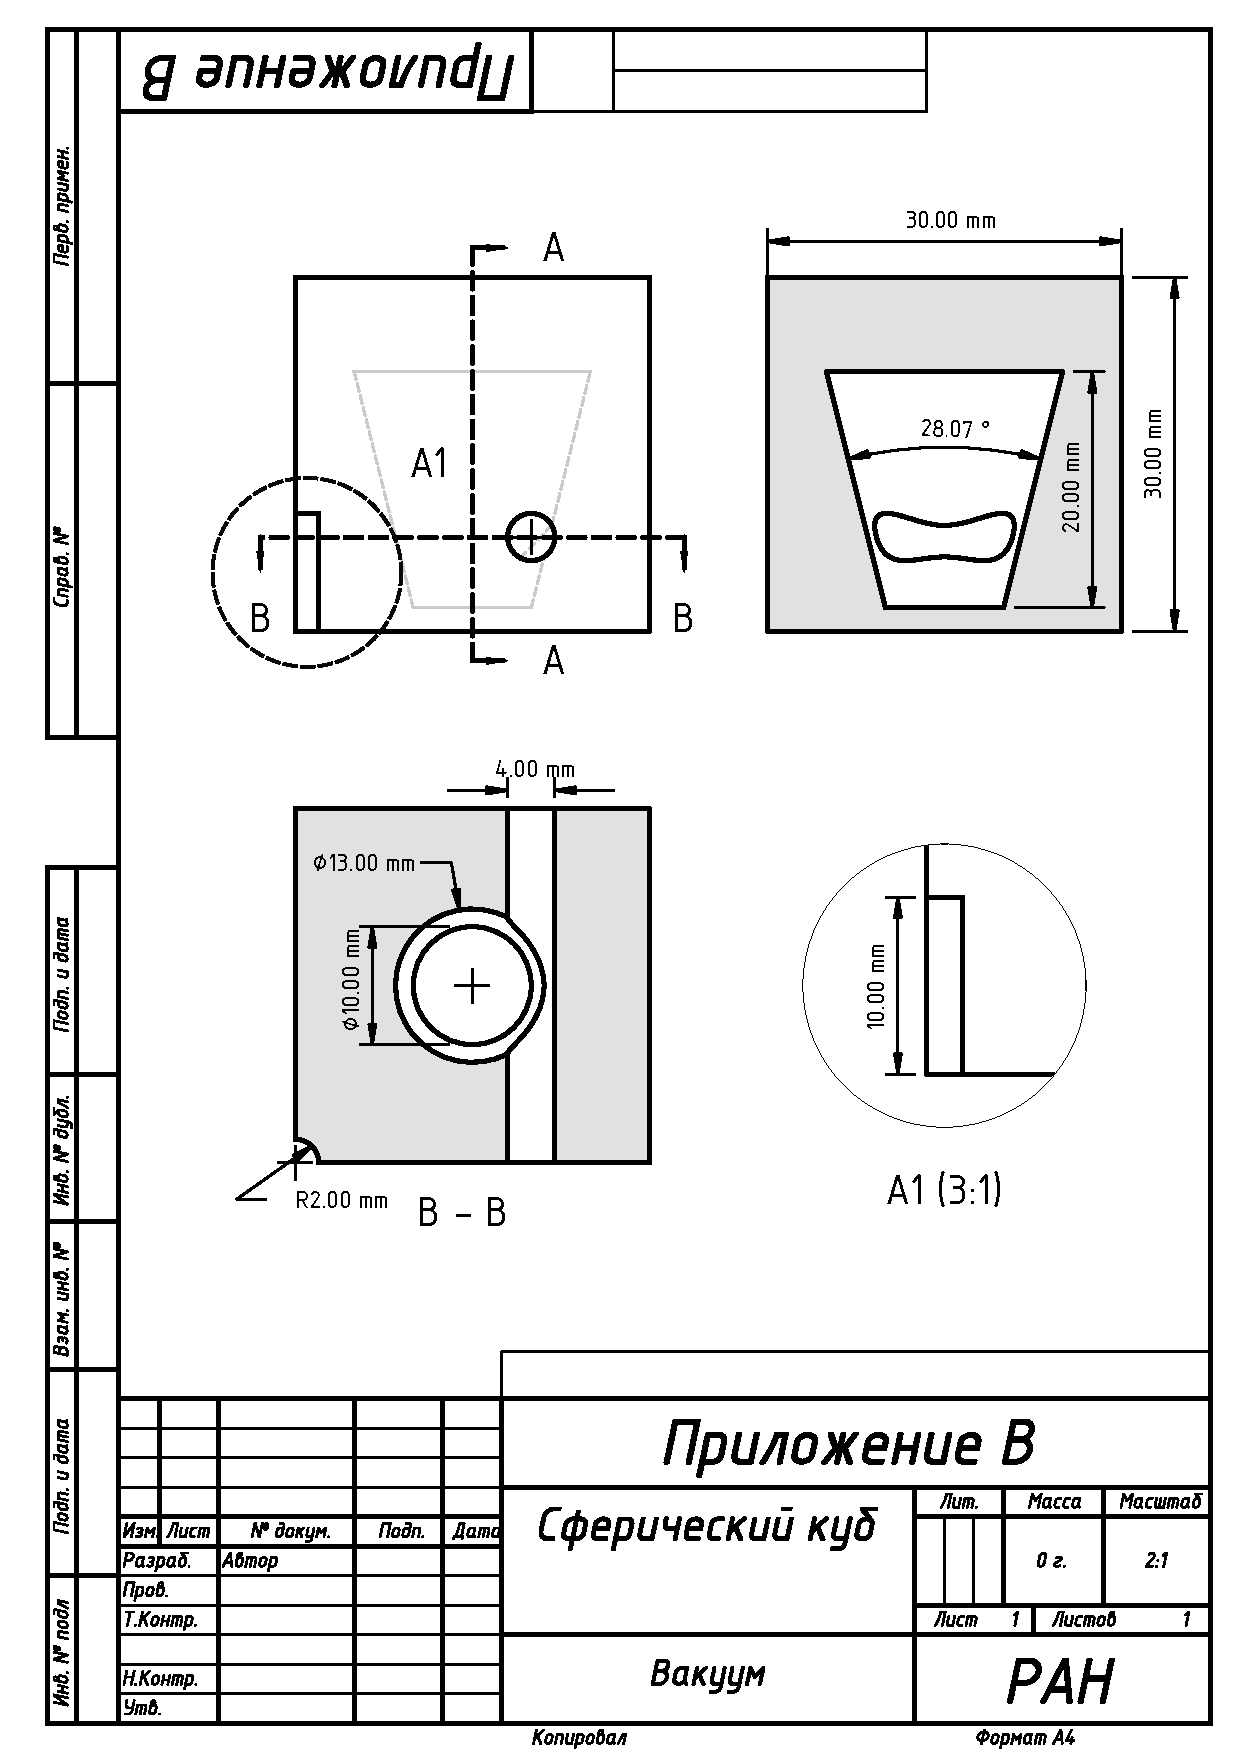
\includepdf[pages=-]{Dissertation/images/drawing.pdf}
        % Приложения

\setcounter{totalappendix}{\value{chapter}} % Подсчёт количества приложений

\end{document}
